\documentclass[11pt,a4paper]{article}
% ============================================================
%  Shared preamble for the Medical Signal and Image Processing
%  Lab reports (English edition).  Compile with pdfLaTeX.
% ============================================================
\usepackage[T1]{fontenc}
\usepackage[utf8]{inputenc}
\usepackage{mathpazo}                     % Palatino text and math
\usepackage[scaled=0.92]{helvet}          % sans-serif for headings
\usepackage{courier}                      % monospace for code
\usepackage{amsmath,amssymb,bm}
\usepackage{microtype}
\usepackage[a4paper,left=2.4cm,right=2.4cm,top=2.9cm,bottom=2.5cm,headheight=22pt]{geometry}
\usepackage{xcolor}
\usepackage{graphicx}
\usepackage{float}
\usepackage{placeins}
\usepackage{booktabs,array,multirow,tabularx,longtable}
\usepackage{enumitem}
\usepackage{siunitx}
\usepackage{caption,subcaption}
\usepackage{fancyhdr}
\usepackage{titlesec}
\usepackage{listings}
\usepackage[most]{tcolorbox}
\usepackage{tikz}
\usepackage[colorlinks=true,linkcolor=primary,citecolor=primary,urlcolor=primary]{hyperref}

\linespread{1.06}
\setlength{\parindent}{0pt}
\setlength{\parskip}{0.55em}
\emergencystretch=3em

% ---------- colours ----------
\definecolor{primary}{HTML}{1B6B87}
\definecolor{accent}{HTML}{C2522B}
\definecolor{soft}{HTML}{EAF3F6}
\definecolor{ink}{HTML}{22313A}
\definecolor{muted}{HTML}{6B7A83}

% ---------- headings ----------
\titleformat{\section}
  {\sffamily\bfseries\LARGE\color{primary}}{\thesection}{0.7em}{}
  [{\vspace{-0.2em}\color{primary!35}\titlerule[0.8pt]}]
\titleformat{\subsection}
  {\sffamily\bfseries\large\color{ink}}{\thesubsection}{0.6em}{}
\titleformat{\subsubsection}
  {\sffamily\bfseries\normalsize\color{primary}}{\thesubsubsection}{0.5em}{}
\titlespacing*{\section}{0pt}{1.6em}{0.9em}
\titlespacing*{\subsection}{0pt}{1.3em}{0.5em}
\titlespacing*{\subsubsection}{0pt}{1.0em}{0.3em}

% ---------- header / footer ----------
\pagestyle{fancy}
\fancyhf{}
\renewcommand{\headrulewidth}{0.4pt}
\renewcommand{\headrule}{\hbox to\headwidth{\color{primary!45}\leaders\hrule height \headrulewidth\hfill}}
\fancyhead[L]{\sffamily\small\color{muted}Medical Signal and Image Processing Lab}
\fancyhead[R]{\sffamily\small\color{muted}\reportshorttitle}
\fancyfoot[C]{\sffamily\small\color{muted}\thepage}
\fancypagestyle{plain}{\fancyhf{}\fancyfoot[C]{\sffamily\small\color{muted}\thepage}\renewcommand{\headrulewidth}{0pt}}

% ---------- captions ----------
\captionsetup{font={small,sf},labelfont={bf,color=primary},labelsep=period,
  format=plain,justification=centering,skip=6pt}
\captionsetup[table]{position=above,skip=5pt}
\renewcommand{\arraystretch}{1.18}

% ---------- code listings ----------
\lstdefinestyle{code}{
  basicstyle=\ttfamily\footnotesize,
  keywordstyle=\color{primary}\bfseries,
  commentstyle=\color{muted}\itshape,
  stringstyle=\color{accent},
  backgroundcolor=\color{soft},
  frame=single, rulecolor=\color{primary!30},
  framerule=0.5pt, xleftmargin=0pt, framexleftmargin=4pt,
  aboveskip=0.8em, belowskip=0.6em, breaklines=true,
  showstringspaces=false, columns=fullflexible, keepspaces=true,
  upquote=true, tabsize=2}
\lstset{style=code}

% ---------- boxes ----------
\newtcolorbox{keyresult}[1][]{enhanced,breakable,
  colback=soft,colframe=primary,boxrule=0pt,
  borderline west={3pt}{0pt}{primary},
  arc=2pt,left=10pt,right=10pt,top=7pt,bottom=7pt,
  fonttitle=\sffamily\bfseries,coltitle=primary,
  attach boxed title to top left={yshift=-2mm,xshift=0mm},
  boxed title style={colback=white,boxrule=0pt,top=0pt,bottom=0pt,left=0pt},
  #1}
\newtcolorbox{notebox}[1][]{enhanced,breakable,
  colback=white,colframe=accent!70,boxrule=0pt,
  borderline west={3pt}{0pt}{accent},
  arc=2pt,left=10pt,right=10pt,top=6pt,bottom=6pt,#1}
\newtcolorbox{taskbox}[1][Task]{enhanced,breakable,
  colback=black!4,colframe=black!4,boxrule=0pt,
  borderline west={2.5pt}{0pt}{muted},
  arc=1pt,left=9pt,right=9pt,top=5pt,bottom=5pt,
  fontupper=\small,
  title={\sffamily\bfseries\scriptsize\textcolor{muted}{\MakeUppercase{#1}}},
  coltitle=muted,fonttitle=\sffamily\bfseries\scriptsize,
  attach title to upper={\par\smallskip}}
\newcommand{\pending}[1]{%
  \begin{tcolorbox}[enhanced,colback=white,colframe=white,boxrule=0pt,
    borderline={0.6pt}{0pt}{muted,dashed},arc=2pt,left=8pt,right=8pt,top=5pt,bottom=5pt]
    \sffamily\small\color{muted}Translation pending: #1
  \end{tcolorbox}}

% ---------- question / answer helpers ----------
\newcommand{\question}[2]{%
  \subsection*{\textcolor{accent}{Q#1}\texorpdfstring{\hspace{0.6em}}{ }#2}%
  \addcontentsline{toc}{subsection}{Q#1\texorpdfstring{\quad}{ }#2}}
\newcommand{\answer}{\textbf{\textsf{\textcolor{primary}{Answer.}}}\ }

% ---------- convenient units / symbols ----------
\newcommand{\mV}{\si{\milli\volt}}
\newcommand{\Hz}{\si{\hertz}}

% ---------- title page ----------
% needs: \reportnumber \reporttitle \reportsubtitle
%        \authorone \authortwo \instructor \semester  (authors.tex)
\newcommand{\makereporttitle}{%
  \begingroup
    \thispagestyle{empty}
    \centering
    \vspace*{1.2cm}
    
\includegraphics[width=3.2cm]{sharif-logo.png}\par\vspace{0.9cm}
    {\sffamily\bfseries\Large\color{ink}Sharif University of Technology\par}
    \vspace{0.3cm}
    {\sffamily\large\color{muted}Medical Signal and Image Processing Lab\par}
    \vspace{1.0cm}
    {\color{primary}\rule{0.55\textwidth}{1.2pt}\par}
    \vspace{1.0cm}
    {\sffamily\small\color{accent}\textls[150]{\MakeUppercase{\reportnumber}}\par}
    \vspace{0.5cm}
    {\sffamily\bfseries\fontsize{26}{31}\selectfont\color{primary}\reporttitle\par}
    \vspace{0.6cm}
    {\sffamily\large\color{ink}\reportsubtitle\par}
    \vspace{1.0cm}
    {\color{primary}\rule{0.55\textwidth}{1.2pt}\par}
    \vspace{1.6cm}
    {\sffamily\bfseries\color{muted}\small\textls[100]{PREPARED BY}\par}
    \vspace{0.4cm}
    {\sffamily\Large\color{ink}\authorone\par}
    \vspace{0.2cm}
    {\sffamily\Large\color{ink}\authortwo\par}
    \vspace{1.3cm}
    {\sffamily\color{muted}Instructor:\ \textbf{\color{ink}\instructor}\par}
    \vfill
    {\sffamily\color{muted}\semester\par}
    \vspace{0.8cm}
    \clearpage
  \endgroup}
% inline reference markers such as [1, 2] (the reference list is added in the final part)
\newcommand{\rc}[1]{[#1]}

% Author and course metadata (shared by all reports).
\newcommand{\authorone}{Mohammad Reza Mahdavi}
\newcommand{\authortwo}{Reza Kazemeini Moghaddam}
\newcommand{\instructor}{Marzieh Barakat}
\newcommand{\semester}{Fall Semester 2026}


\newcommand{\reportnumber}{Experiment 2}
\newcommand{\reporttitle}{EEG Noise and Artifact Removal with ICA}
\newcommand{\reportsubtitle}{Simulation at Two Noise Levels and Analysis of Two Real Recordings}
\newcommand{\reportshorttitle}{EEG Noise and Artifact Removal with ICA}

\graphicspath{{figures/}}
\hypersetup{pdftitle={Experiment 2: EEG Noise and Artifact Removal with ICA},pdfauthor={\authorone, \authortwo}}

\begin{document}
\makereporttitle

\section*{Abstract and Reading Guide}
\addcontentsline{toc}{section}{Abstract and Reading Guide}

In this experiment, the removal of EEG noise and artifacts with independent component decomposition was examined. In the simulation part, the desired 32-channel signal was combined with the supplied noise at SNRs of $-5$ and $-15$ decibels. The COM2R algorithm was then run, and the sources with spiky characteristics were selected for reconstruction. The RRMSE decreased from 1.778 to 0.715 and from 5.623 to 2.084. The second result, despite the improvement relative to the input, still has a large error; it shows that noise reduction is not necessarily accompanied by complete preservation of the spikes.

In the real-data part, two recordings, NewData1 and NewData3, were examined. In the first recording, a component with narrow-band interference near 60~Hz was removed; in the second, a component with a probable eye-blink pattern and a component with localized high-frequency contamination were removed. The decisions were based on the simultaneous examination of the time course, the spectrum and the spatial pattern. Because there is no clean reference for the real data, the before-and-after indices are purely descriptive and are not interpreted as reconstruction accuracy.

\bigskip
\tableofcontents
\clearpage

\section{Objective and Background of the Experiment}

The objective is to answer two different problems posed in the exercise: recovering spiky sources from a simulated observation, and removing components with artifactual evidence from real EEG. In the first case a clean reference is available and the error can be measured; in the second, the decisions rely on indirect evidence and on the principle of keeping ambiguous components. The criterion for selecting components was therefore not taken to be the same in these two parts \rc{1, 2}.

\subsection*{Mixing model and the role of ICA}
\begin{equation}
x(t)=A\,s(t)+n(t)
\end{equation}
In this model, the observation vector $x$ is the result of a linear combination of the sources $s$ with the matrix $A$, plus a noise term $n$. In the ICA approximation, the contribution of the separable sources is modeled in the part $As$; the CoM2 method uses fourth-order statistics to find approximately independent components. Statistical independence is not the same as physiological cleanliness, and each component must be examined separately. The order, sign and scale of the sources are also inherently ambiguous, and a component number in two different runs does not necessarily refer to one source \rc{3}.

EEG artifacts can have an ocular, muscular, cardiac or non-physiological origin, such as equipment interference and electrode movement. In epileptic data, sharpness or a high kurtosis alone is not a reason for a component to be undesirable; removal without sufficient evidence can destroy the desired event. For this reason, ambiguous components were kept in the real data \rc{2}.

\subsection*{Choice of algorithm}

The only algorithm of this experiment is CoM2, in the implementation accompanying the exercise, COM2R. This code first performs whitening and the determination of the data subspace with SVD, and then pursues the separation, based on fourth-order statistics, with pairwise rotations. The first output is the mixing matrix $A$, and the second output, $W$, equals the pseudoinverse of $A$. The code runs with a fixed number of sweeps: 7 sweeps for 32 channels and 6 sweeps for 21 channels; a stopping rule based on a convergence threshold is not defined in this implementation \rc{3, COM2R code}.

FastICA, Infomax, JADE and SOBI are other theoretical options, but in the present results they were neither run nor compared with COM2R. Component classifiers such as ICLabel were also not used in this experiment; the labels or probabilities that such tools generate are therefore not attributed to the results.

\section{Data and Method of Execution}

\begin{center}
\begin{tabular}{@{}lccc@{}}
\toprule
\textbf{Set} & \textbf{Matrix size} & \textbf{Sampling rate} & \textbf{Last value of the time axis}\\
\midrule
\texttt{X\_org} and \texttt{X\_noise} & $32\times10240$ & 250 Hz & 40.956 s\\
NewData1 & $21\times1251$ & 250 Hz & 5.000 s\\
NewData3 & $21\times1251$ & 250 Hz & 5.000 s\\
\bottomrule
\end{tabular}
\end{center}

In the simulation, the sampling rate was taken from the file \texttt{plotEEG} accompanying the data, and in the real-data part from the exercise. The time axis was built with $t=(0{:}N{-}1)/f_s$; for example, $N/f_s$ in the simulation is 40.96 seconds, but the last sample on the axis lies at 40.956 seconds. Since amplitude calibration specifications are not available in the data, the unit of the plots is given as a.u.\ and microvolts are not assumed.

\subsection*{Mean removal and rank}
\begin{equation}
X_c = X-\mu\mathbf{1}^{T};\qquad S=WX_c;\qquad W=A^{+}
\end{equation}
Before ICA, only the mean of each channel was removed from the same observation. A band-pass filter, notch filter, channel removal, change of reference and standardization of the channels were not applied. The numerical rank of the mean-removed data was examined with SVD and was 32 for the simulation and 21 for each real recording. After the reconstruction, the mean of the observation was added back. The frequency bands mentioned below serve only for feature extraction and do not mean filtering the data in those bands.

\subsection*{Spectrum estimation and features}

The PSD was computed with \texttt{pwelch}, using a Hamming window of 500 samples (equal to 2 seconds), an overlap of 250 samples and an NFFT of 1024. The spacing of the points of the frequency grid is about 0.244~Hz; this spacing results from the zero-padded grid and must not be regarded as an independent spectral resolution. The effective resolution also depends on the length and shape of the window \rc{4}.
\begin{equation}
\mathrm{HF}=\frac{\int_{30}^{100}P(f)\,df}{\int_{0.5}^{100}P(f)\,df};\qquad
\mathrm{LF}=\frac{\int_{0.5}^{4}P(f)\,df}{\int_{0.5}^{100}P(f)\,df}
\end{equation}
HF and LF are the ratios of the power of the band of interest to the power in 0.5 to 100~Hz. The Line60 index likewise describes the share of the power in 59 to 61~Hz with the same denominator. The excess kurtosis, the maximum absolute normalized $z$, the squared-weight share of the map in the frontal channels, the concentration of the maximum of the map and the correlation of adjacent samples were computed as descriptive evidence; these indices are not valid probabilities of artifact detection.

For each component, $z$ is obtained by subtracting the temporal mean of that component and dividing by its root mean square after the mean removal; this normalization is used only in feature extraction.
\begin{equation}
\kappa=E[z^{4}]-3
\end{equation}

\section{Part 1: Denoising of Simulated Data}

\begin{taskbox}[Part 1: introduction in the lab manual]
In this part we want to use the ICA method to study the removal of noise from a simulated EEG signal (the data of this part are in the folder \texttt{Lab2\_1}). Since the clean data (the desired signal) are available in the simulated signal, different algorithms can be evaluated and compared with quantitative metrics. For this purpose a 32-channel interictal (non-seizure) epileptic EEG signal is used. This realistic simulated data is the noise-free data (the desired signal), the matrix \texttt{X\_org}. A real signal containing muscle noise and background EEG is also given (\texttt{noise\_X}). We want to add the noise to the desired signal at different SNRs and then reconstruct the desired signal with blind source separation algorithms.
\end{taskbox}

\subsection*{Question 1: Plotting the clean signal}
\begin{taskbox}
Plot the noise-free signal \texttt{X\_org}. Label the channels and the time. You can use the files \texttt{plotEEG.m} and \texttt{eeg\_disp.m}. For a better display, you can tune the variable \texttt{offset} (the spacing between the signals shown for two channels).
\end{taskbox}

The matrix \texttt{X\_org} contains the desired 32-channel data. Figure~\ref{fig:xorg} shows all channels with their labels and the time axis. Sharp, few events can be seen on the background. According to the definition in the exercise, this data is simulated and interictal; no new clinical conclusion is inferred from it. For the stacked display, the mean of each channel was subtracted and a fixed vertical offset was added; this offset is only for display.

\begin{figure}[H]
\centering
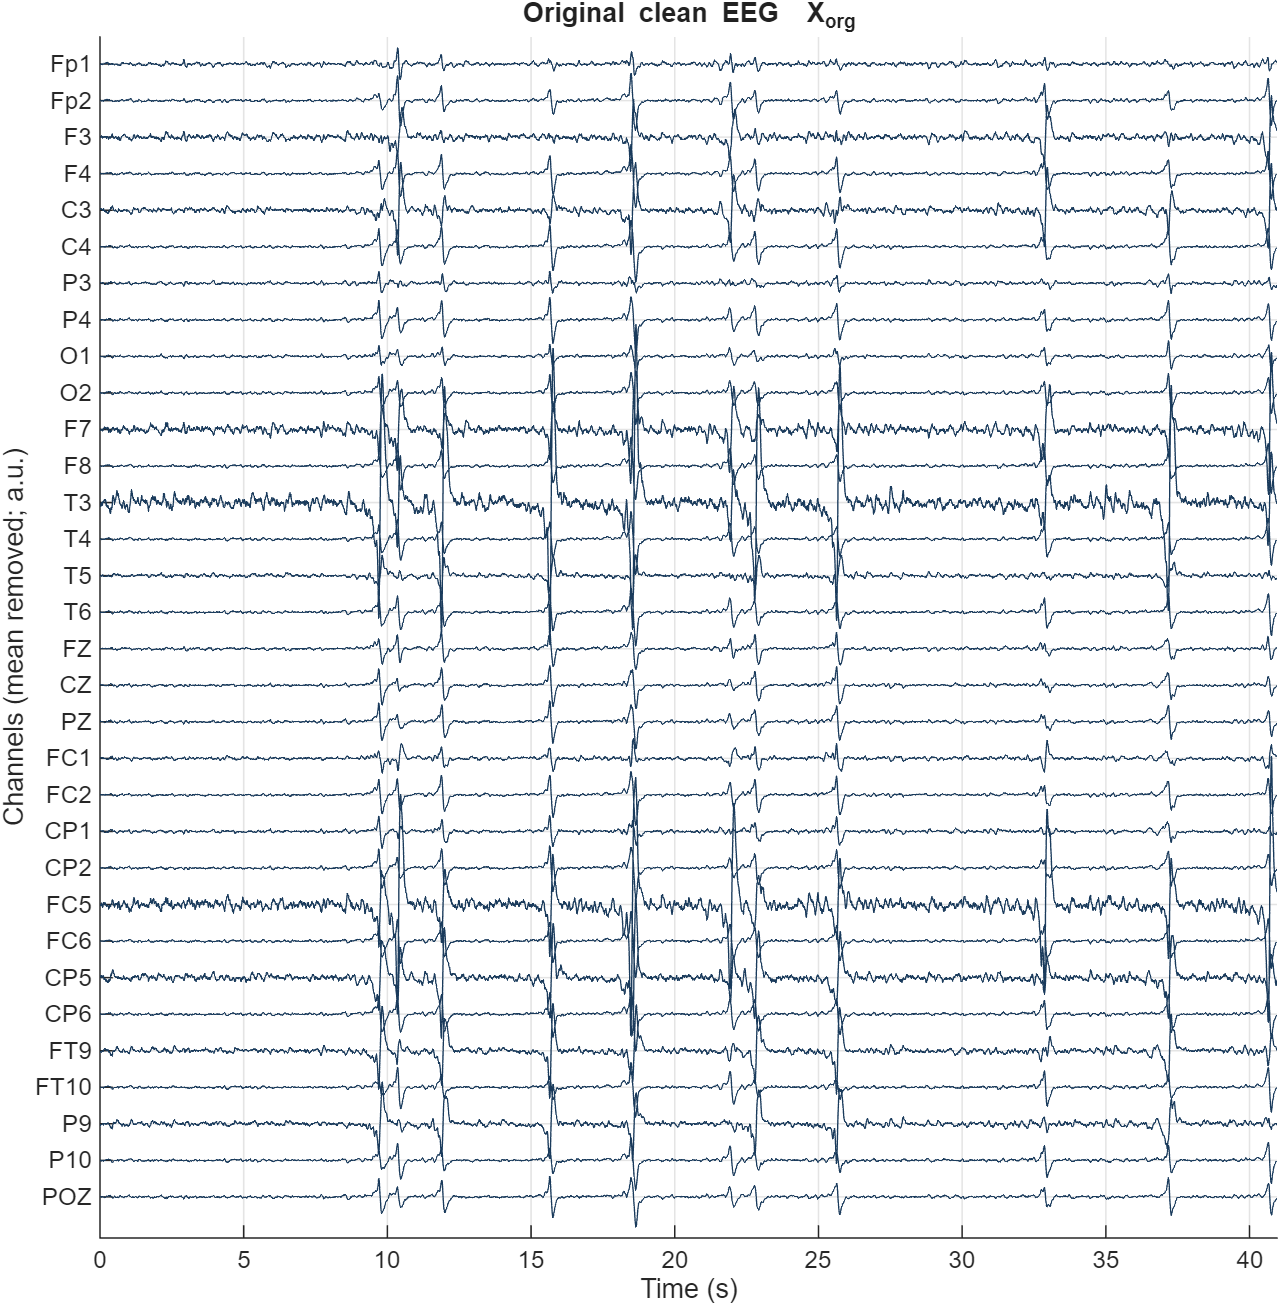
\includegraphics[width=0.85\textwidth,height=0.72\textheight,keepaspectratio]{fig01_clean_eeg_xorg.png}
\caption{The desired signal \texttt{X\_org} with the labels of all 32 channels and the time axis in seconds.}
\label{fig:xorg}
\end{figure}

\subsection*{Question 2: Examining the supplied noise}
\begin{taskbox}
Plot the noise \texttt{X\_noise}. Label the channels and the time.
\end{taskbox}

Figure~\ref{fig:xnoise} shows \texttt{X\_noise} itself, without multiplication by the noise coefficient. According to the exercise, this data contains background EEG and muscle contamination. The change of amplitude and the temporal envelope show that the noise is not necessarily stationary, and in some intervals faster and more clustered activity is seen. The noise should therefore not be assumed to be merely white Gaussian noise. Its contribution to the observation is determined after multiplication by a coefficient common to all channels.

\begin{figure}[H]
\centering
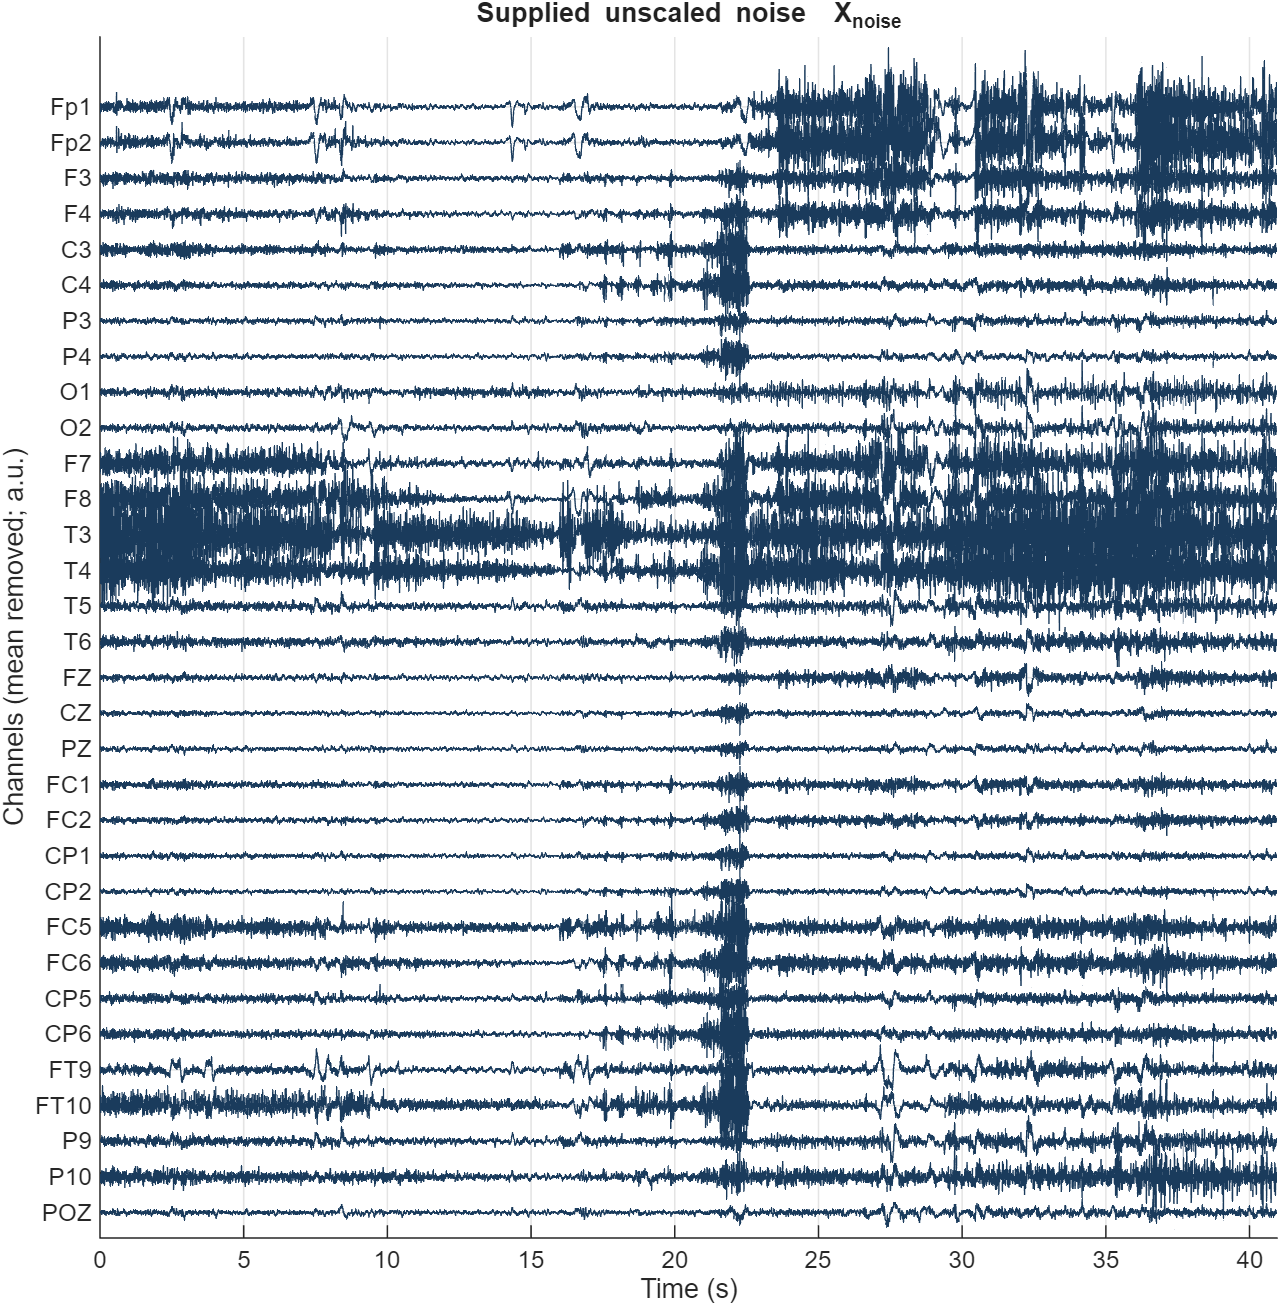
\includegraphics[width=0.85\textwidth,height=0.72\textheight,keepaspectratio]{fig02_noise_xnoise.png}
\caption{The raw noise \texttt{X\_noise} without scaling; the vertical spacing of the channels is only for readability.}
\label{fig:xnoise}
\end{figure}

\subsection*{Question 3: Building the observation at a specified SNR}
\begin{taskbox}
Add the noise to the original signal at different SNRs ($-5$~dB and $-15$~dB) and build the observation signal. Plot the noisy signal for $\mathrm{SNR}=-15$~dB and compare it with the noise-free signal. (The manual defines $\mathrm{SNR}_{dB}=10\log_{10}(P_{\mathrm{signal}}/P_{\mathrm{noise}})$; for a multichannel signal, $\mathbf{x}[m]=\mathbf{s}[m]+\sigma\mathbf{N}[m]$ with one $\sigma$ common to all channels, i.e.\ $\sigma^{2}=\frac{P_s}{P_N}\times10^{-\mathrm{SNR}_{dB}/10}$.)
\end{taskbox}

\begin{align}
X &= X_{\mathrm{org}}+\sigma X_{\mathrm{noise}}\\
\mathrm{SNR}_{dB} &= 10\log_{10}\!\left(\frac{\|X_{\mathrm{org}}\|_F^{2}}{\sigma^{2}\|X_{\mathrm{noise}}\|_F^{2}}\right)\\
\sigma &= \frac{\|X_{\mathrm{org}}\|_F}{\|X_{\mathrm{noise}}\|_F}\times10^{-\mathrm{SNR}_{dB}/20}
\end{align}

A common coefficient $\sigma$ was used for all channels. For an SNR of $-5$~dB, $\sigma$ equals 3.582232, and for $-15$~dB it equals 11.328013. The SNR measured after the addition was $-5$ and $-15$~dB, respectively. The ratio of the noise power to the desired-signal power in these two cases is about 3.16 and 31.62; the noise amplitude of the second case relative to the first is about $\sqrt{10}$ times larger.

\begin{lstlisting}[language=Matlab]
sigma = norm(X_org,'fro') / norm(X_noise,'fro') ...
        * 10^(-targetSNR/20);
X = X_org + sigma * X_noise;
\end{lstlisting}

Figure~\ref{fig:noisy15} shows the $-15$~dB observation. As the noise increases, identifying the desired events becomes more difficult in many channels. The exact comparison of amplitudes is made in the overlaid figures of channels 13 and 24; the vertical spacing of the stacked plots alone is not a measure of the SNR.

\begin{figure}[H]
\centering
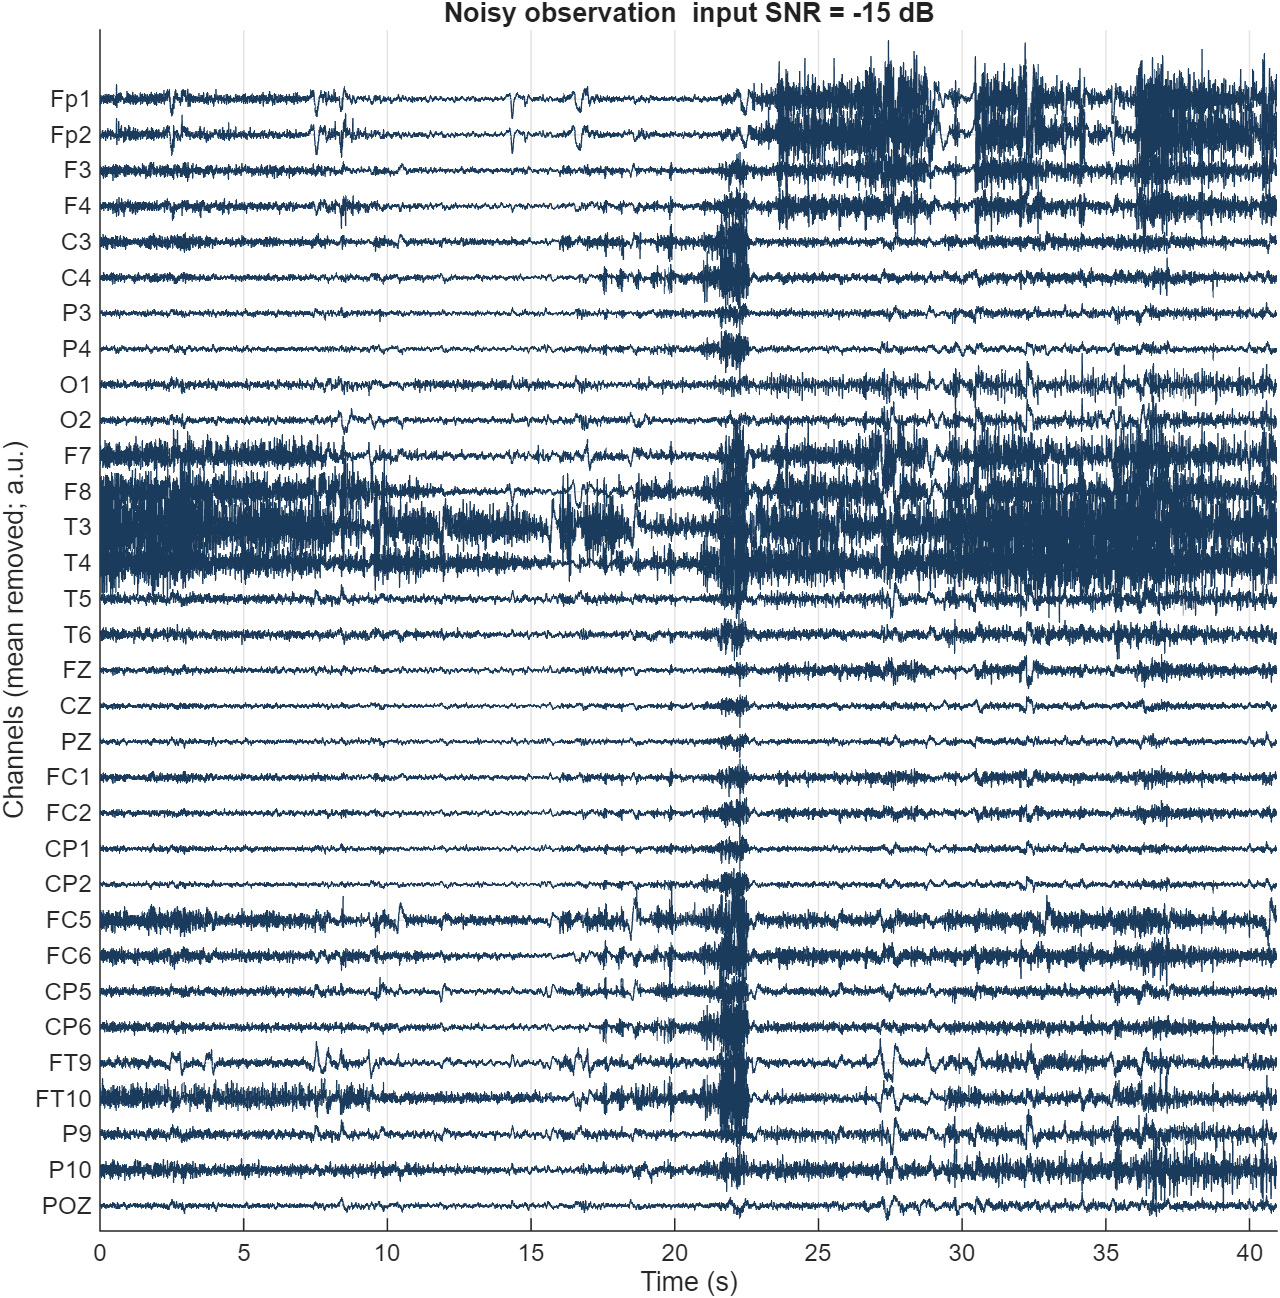
\includegraphics[width=0.85\textwidth,height=0.72\textheight,keepaspectratio]{fig03_noisy_observation_m15db.png}
\caption{The noisy observation at an SNR of $-15$~dB; all channels are labeled.}
\label{fig:noisy15}
\end{figure}

\subsection*{Questions 4 and 5: Separation and selection of the sources}
\begin{taskbox}
\textbf{4.} Extract the sources using an ICA method of your choice. You can use the function \texttt{R2COM.m} (the R2Com algorithm).\\
\textbf{5.} Examine all the obtained sources, keep the desired sources (spiky sources), and remove the other sources.
\end{taskbox}

For each SNR, the COM2R algorithm was run separately on the mean-removed observation, which has full rank. The size of $A$ and $W$ is $32\times32$ and the size of $S$ is $32\times10240$. All components were examined in time, frequency and mixing weights; the complete sheets are given in Appendix~C. The IC numbers of the two SNRs belong only to their own decomposition and must not be assumed to correspond one to one.

\begin{lstlisting}[language=Matlab]
channelMean = mean(X,2);
Xc = X - channelMean;
[A,W,sweeps] = COM2R(Xc,32);
S = W * Xc;
\end{lstlisting}

For a transparent and reproducible record of the selection of the spiky sources, the following three simultaneous conditions were used. The thresholds are an instructional, data-specific rule and are not a boundary for medical diagnosis. \texttt{X\_org} was not used to tune these selections; it served only as the reference for computing the error and comparing the figures.
\begin{equation}
\kappa\ge 6;\qquad \max_t|z(t)|\ge 6;\qquad \mathrm{HF}\le 0.20
\end{equation}

\begin{center}
\begin{tabular}{@{}lcc@{}}
\toprule
\textbf{Input SNR} & \textbf{Kept components} & \textbf{Kept / removed}\\
\midrule
$-5$ dB  & 2\ 5\ 9\ 10\ 12\ 21\ 23\ 32 & 8 / 24\\
$-15$ dB & 7\ 8\ 18\ 20\ 30\ 32        & 6 / 26\\
\bottomrule
\end{tabular}
\end{center}

Kurtosis alone is not sufficient: for example, at $-5$~dB component 6, with a kurtosis of about 109.6 and a high-frequency share of about 0.778, was removed; despite its sharpness and high kurtosis, its activity is a high-frequency burst. Conversely, keeping a component with a sharp event does not guarantee that the component is completely free of background or noise. The large error of the $-15$~dB case shows the limitation of this very separation and of the selection rule.

In this part, the aim of the exercise is to keep the spiky sources and set aside the other sources. In the real-data part, the aim is to preserve the brain components and remove only those with artifactual evidence; the selection rule of the simulation was therefore not generalized to the real data.

\subsection*{Questions 6 and 7: Reconstruction and comparison of the channels}
\begin{taskbox}
\textbf{6.} Project the desired sources back to the sensor domain (the observation domain) and build the denoised observations (\texttt{X\_den}).\\
\textbf{7.} Plot the denoised observations for channels 13 and 24 together with the original noise-free data and the noisy data.
\end{taskbox}

\begin{equation}
X_{\mathrm{den}}=A(:,K)\,S(K,:)+\mu\mathbf{1}^{T}
\end{equation}
After selecting the set $K$, i.e.\ \texttt{SelSources}, only the contribution of those components was returned to the sensor space. The mean term was added because of the earlier mean removal, and it is consistent with the exercise formula for mean-removed data. Channel 13 in this data is T3 and channel 24 is FC5. At $-5$~dB, the reconstruction follows many of the reference events, but differences in the background and in the amplitude remain.

\begin{figure}[H]
\centering
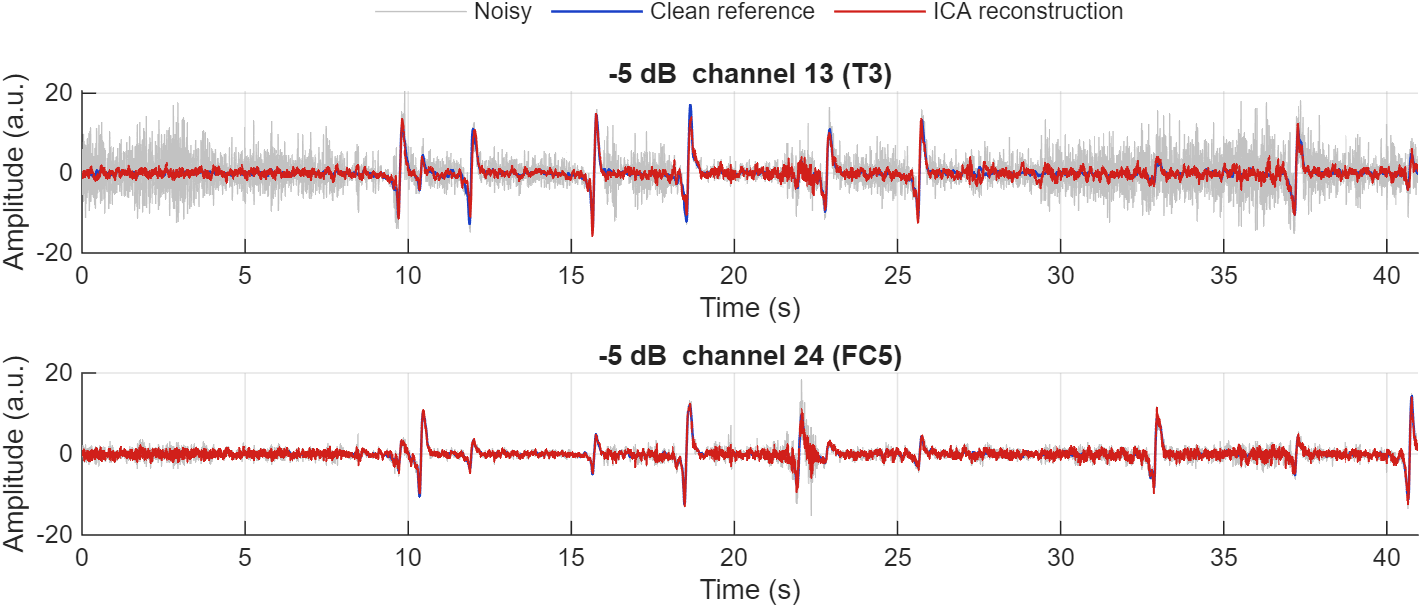
\includegraphics[width=\textwidth]{fig04_channels_t3_fc5_m5db.png}
\caption{Comparison of channels T3 and FC5 at $-5$~dB; gray is the observation, blue is the clean reference and red is the reconstruction.}
\label{fig:ch5}
\end{figure}

\begin{figure}[H]
\centering
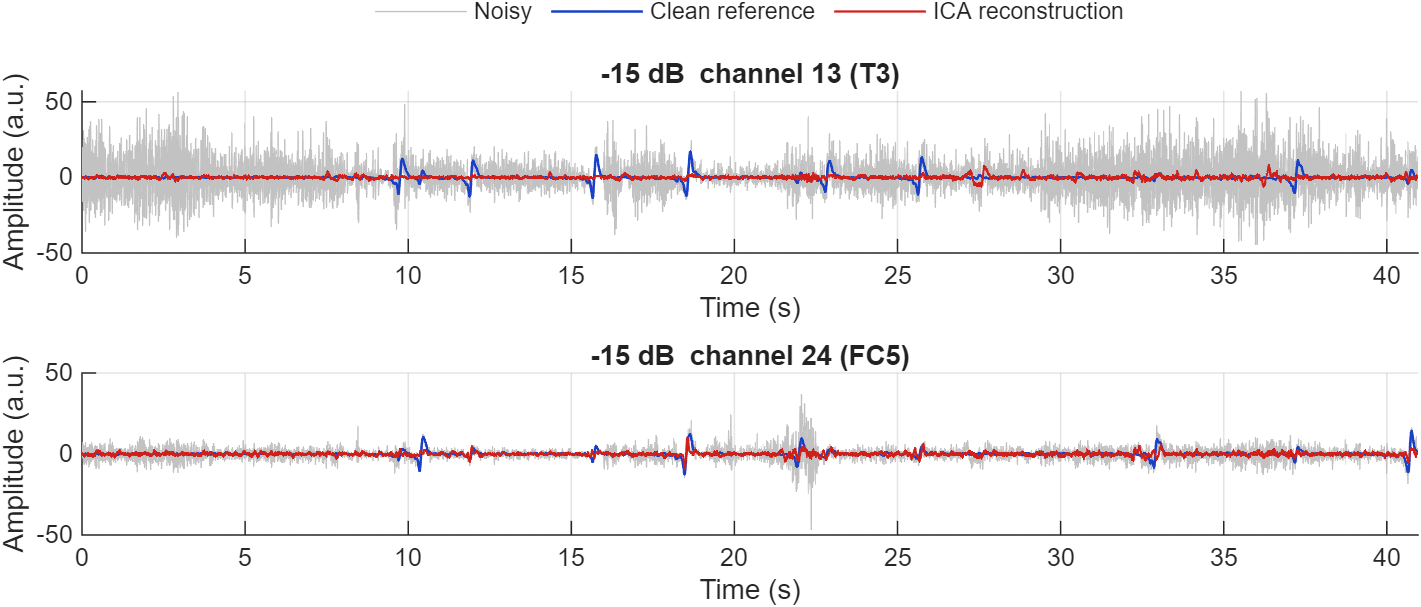
\includegraphics[width=\textwidth]{fig05_channels_t3_fc5_m15db.png}
\caption{The same comparison at $-15$~dB; part of the reference spikes, especially in T3, has not been recovered well.}
\label{fig:ch15}
\end{figure}

\paragraph{Temporal detail and error of the selected channels.} The zooms are shown around the largest reference event of channel 13; the location of the zoom was not used to select the components. Under strong noise, an apparent smoothing of the output does not necessarily mean preservation of the desired event. Both the waveform shape and the numerical error must be examined.

\begin{figure}[H]
\centering
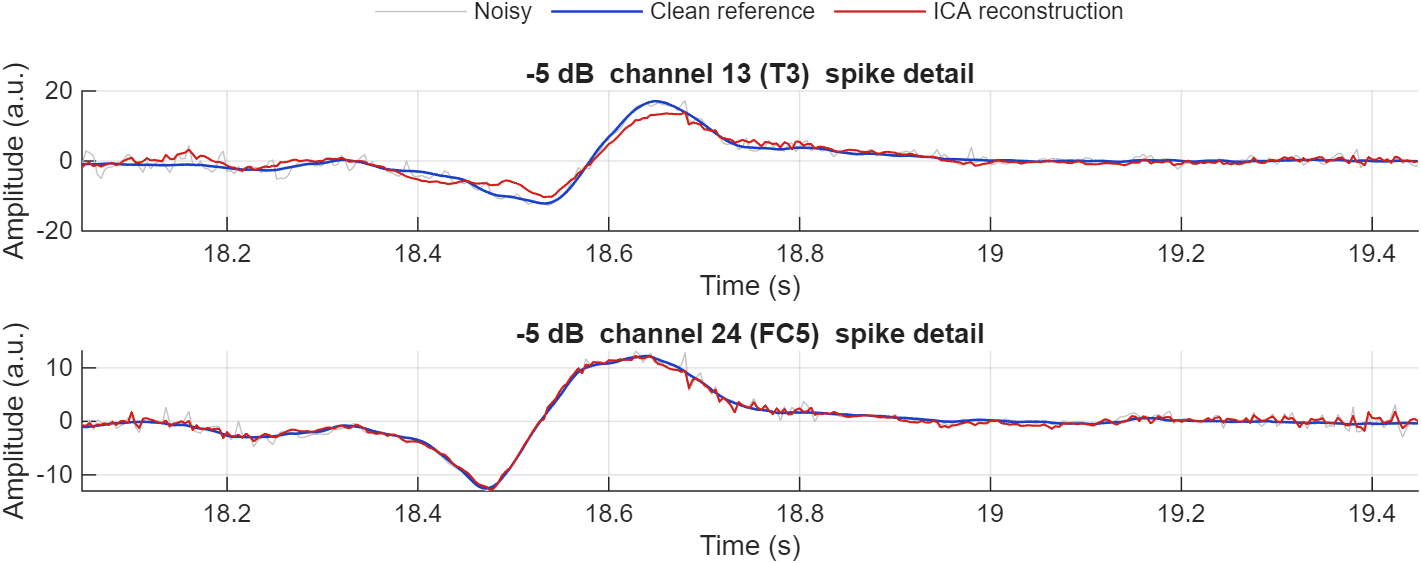
\includegraphics[width=0.95\textwidth]{fig06_event_detail_m5db.png}
\caption{Detail of an event at $-5$~dB; comparison of the shape and amplitude of the reconstruction with the reference.}
\label{fig:det5}
\end{figure}

\begin{figure}[H]
\centering
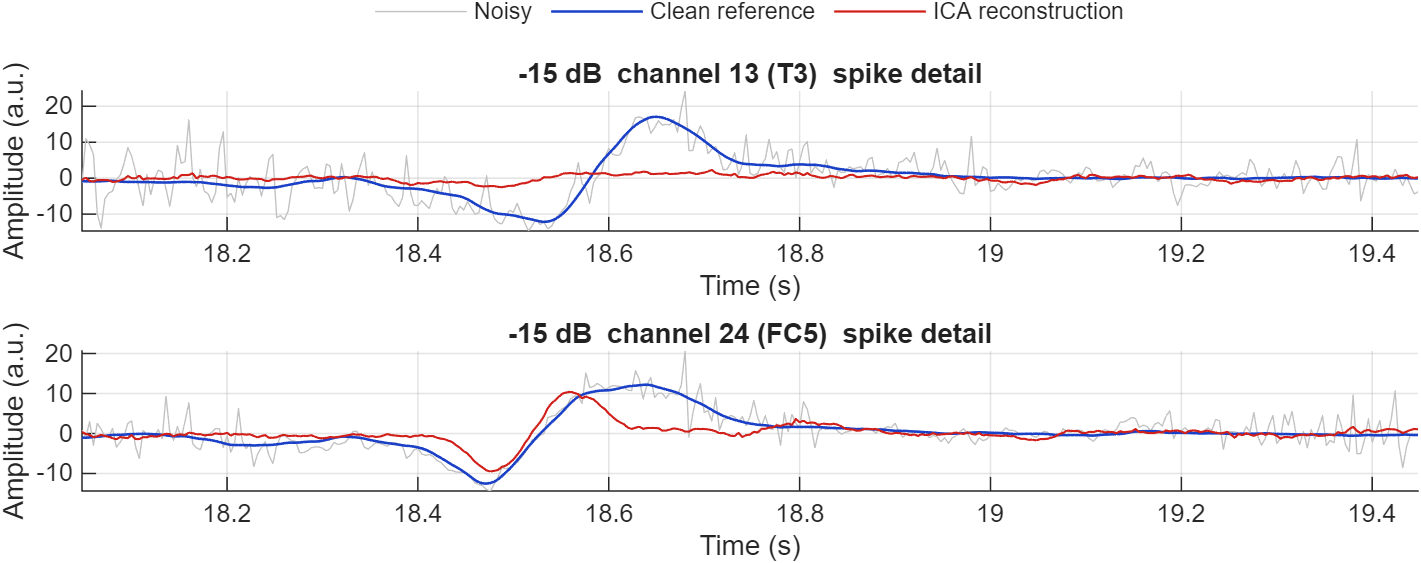
\includegraphics[width=0.95\textwidth]{fig07_event_detail_m15db.png}
\caption{Detail of the same interval at $-15$~dB; the difference between the reconstruction and the reference is more evident.}
\label{fig:det15}
\end{figure}

\begin{center}
\begin{tabular}{@{}clcc@{}}
\toprule
\textbf{SNR} & \textbf{Channel} & \textbf{Input RRMSE} & \textbf{Output RRMSE}\\
\midrule
$-5$ dB  & 13 T3  & 1.442288 & 0.416973\\
$-5$ dB  & 24 FC5 & 0.581928 & 0.367643\\
$-15$ dB & 13 T3  & 4.560914 & 1.044193\\
$-15$ dB & 24 FC5 & 1.840218 & 0.963348\\
\bottomrule
\end{tabular}
\end{center}

\subsection*{Question 8: Computing and analyzing the RRMSE}
\begin{taskbox}
Compute the RRMSE (relative RMSE) for each SNR. Analyze the obtained results. (The manual defines $\mathrm{RRMSE}=\sqrt{\sum_{n=1}^{32}\sum_{t=1}^{T}(x_{org}^{(n)}(t)-x_{den}^{(n)}(t))^2}\big/\sqrt{\sum_{n=1}^{32}\sum_{t=1}^{T}(x_{org}^{(n)}(t))^2}$.)
\end{taskbox}

\begin{align}
\mathrm{RRMSE}&=\frac{\|X_{\mathrm{org}}-X_{\mathrm{den}}\|_F}{\|X_{\mathrm{org}}\|_F}\\
\mathrm{SNR}_{\mathrm{out}}&=-20\log_{10}(\mathrm{RRMSE})
\end{align}
The RRMSE is the ratio of the Frobenius norm of the error to the Frobenius norm of the reference, and it is computed from the sum over the samples and the channels; this value is not the mean RRMSE of the channels. The relation of the output SNR to the RRMSE also holds with this same reference and the same definition of the error.

\begin{center}
\small
\begin{tabular}{@{}cccccc@{}}
\toprule
\textbf{Input SNR} & $\sigma$ & \textbf{Input RRMSE} & \textbf{Output RRMSE} & \textbf{Output SNR} & \textbf{SNR improvement}\\
\midrule
$-5$ dB  &  3.582232 & 1.778279 & 0.714724 &  2.9172 dB & 7.9172 dB\\
$-15$ dB & 11.328013 & 5.623413 & 2.084281 & $-6.3791$ dB & 8.6209 dB\\
\bottomrule
\end{tabular}
\end{center}

\begin{figure}[H]
\centering
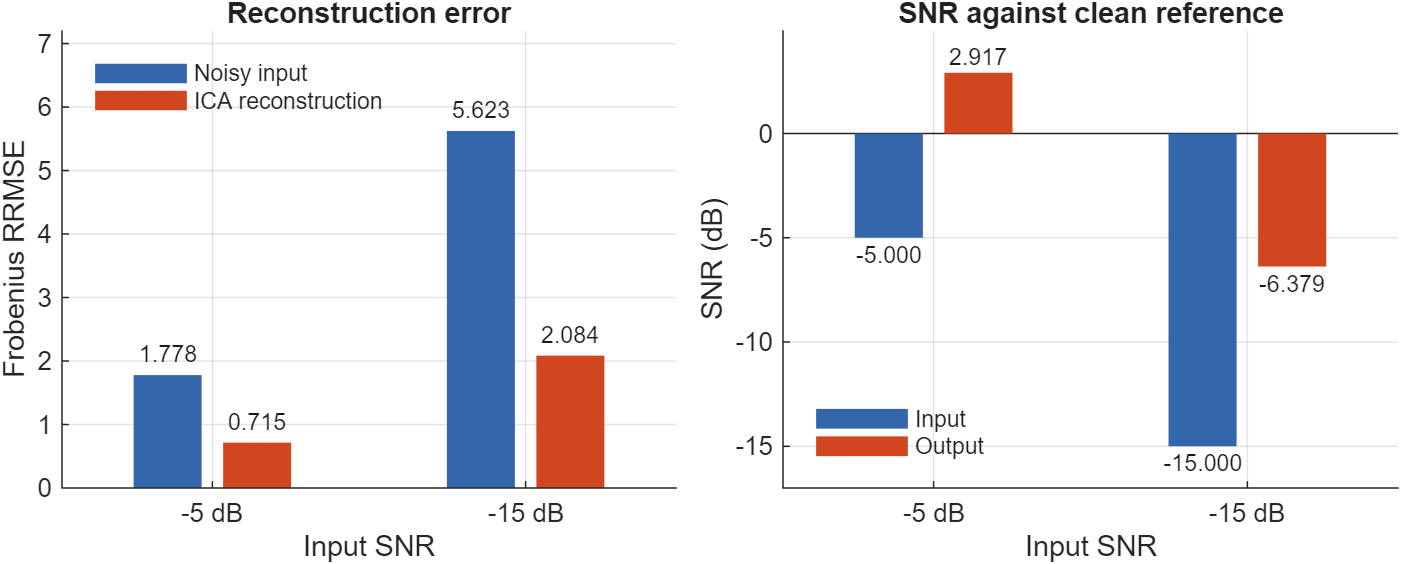
\includegraphics[width=0.95\textwidth]{fig08_rrmse_and_snr.png}
\caption{Comparison of the relative error and the SNR; both cases improve relative to the observation, but the absolute quality of the $-15$~dB case is lower.}
\label{fig:rrmse}
\end{figure}

The relative reduction of the error norm with respect to the input is about 59.8 percent and 62.9 percent. These percentages are not ``accuracy'' or ``percent of the signal recovered.'' In the $-15$~dB case, the output RRMSE is 2.084 and the output SNR is still $-6.379$~dB; the residual error energy is about 4.34 times the energy of the clean reference. For comparison, an all-zero estimate has an RRMSE of one. Consequently, the improvement relative to the very noisy observation is not sufficient to consider the reconstruction of this case adequate.

This result is consistent with the presence of mixed sources, the dominance of noise, and the loss or attenuation of some spikes. The larger improvement in dB in the noisier case must not be confused with the output being better. Tuning the selections by using the clean reference directly could have reduced the error of the same data, but it would have made the evaluation of blind separation optimistic; such tuning was not performed.

\paragraph{Spectral examination of the simulation reconstruction.} Figure~\ref{fig:psdsim} shows the mean PSD of the channels at the two SNRs.

\begin{figure}[H]
\centering
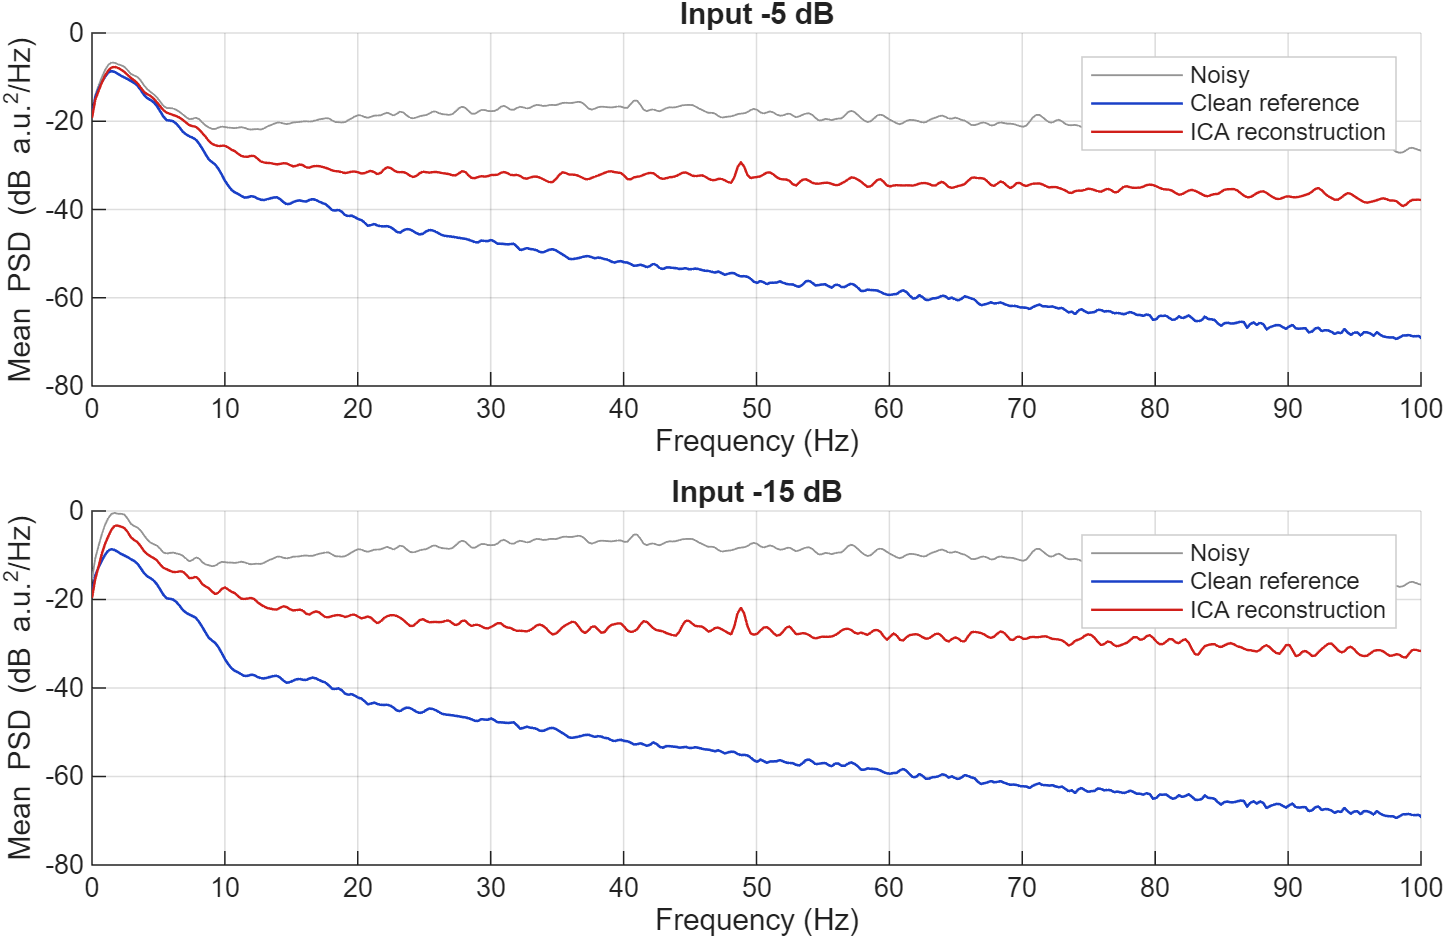
\includegraphics[width=0.9\textwidth]{fig09_psd_simulation.png}
\caption{Mean PSD of the channels at the two SNRs; a decrease of high-frequency power alone does not prove preservation of the spike shape.}
\label{fig:psdsim}
\end{figure}

The PSD plot shows that the reconstruction has reduced a considerable share of the observation power, especially at higher frequencies. However, the PSD does not completely preserve the information on the phase and the exact timing of events. Two signals with similar spectra can have different temporal shapes; spectral analysis was therefore used alongside the waveform and the RRMSE.

The residual of the reconstruction using all components was about $3.87\times10^{-12}$ and $4.69\times10^{-12}$. These small values confirm the consistency of the matrices $A$ and $W$ and of the back-mapping; they do not prove complete statistical independence, the biological correctness of the components, or the quality of the noise removal.

\section{Part 2: Examination of the Real Data NewData1}

\begin{taskbox}[Part 2: introduction in the lab manual]
The folder of this experiment (\texttt{Lab2\_2}) contains four \texttt{.mat} files with EEG signals (\texttt{NewData1} to \texttt{NewData4}). The signals belong to epileptic patients and were recorded in seizure or non-seizure periods (sampling frequency 250~Hz). The goal is to remove the noise and artifacts of the given signals using the ICA method. Choose two of the four signals and carry out the following steps for each of them.
\end{taskbox}

\subsection*{Questions 1 and 2: Observation and identification of the artifact pattern}
\begin{taskbox}
\textbf{1.} Plot the signal in the time domain, labeling all channels.\\
\textbf{2.} Examine the signal for noise and artifacts. What type of artifact do you see in the signal? In your opinion, can this artifact be removed using the ICA method?
\end{taskbox}

The NewData1 recording consists of 21 channels and the interval from zero to five seconds. Figure~\ref{fig:nd1} shows the original data and the reconstruction with identical vertical spacing and axis range. In some channels a relatively continuous fast oscillation is seen. In the ICA decomposition, component 4 has an oscillatory time course and a narrow peak at 60.059~Hz; about 75.1 percent of its power in 0.5--100~Hz lies in the band 59 to 61~Hz. This evidence is consistent with narrow-band interference near 60~Hz. The exact origin of the equipment or the recording location is not determined from this data alone.

\begin{figure}[H]
\centering
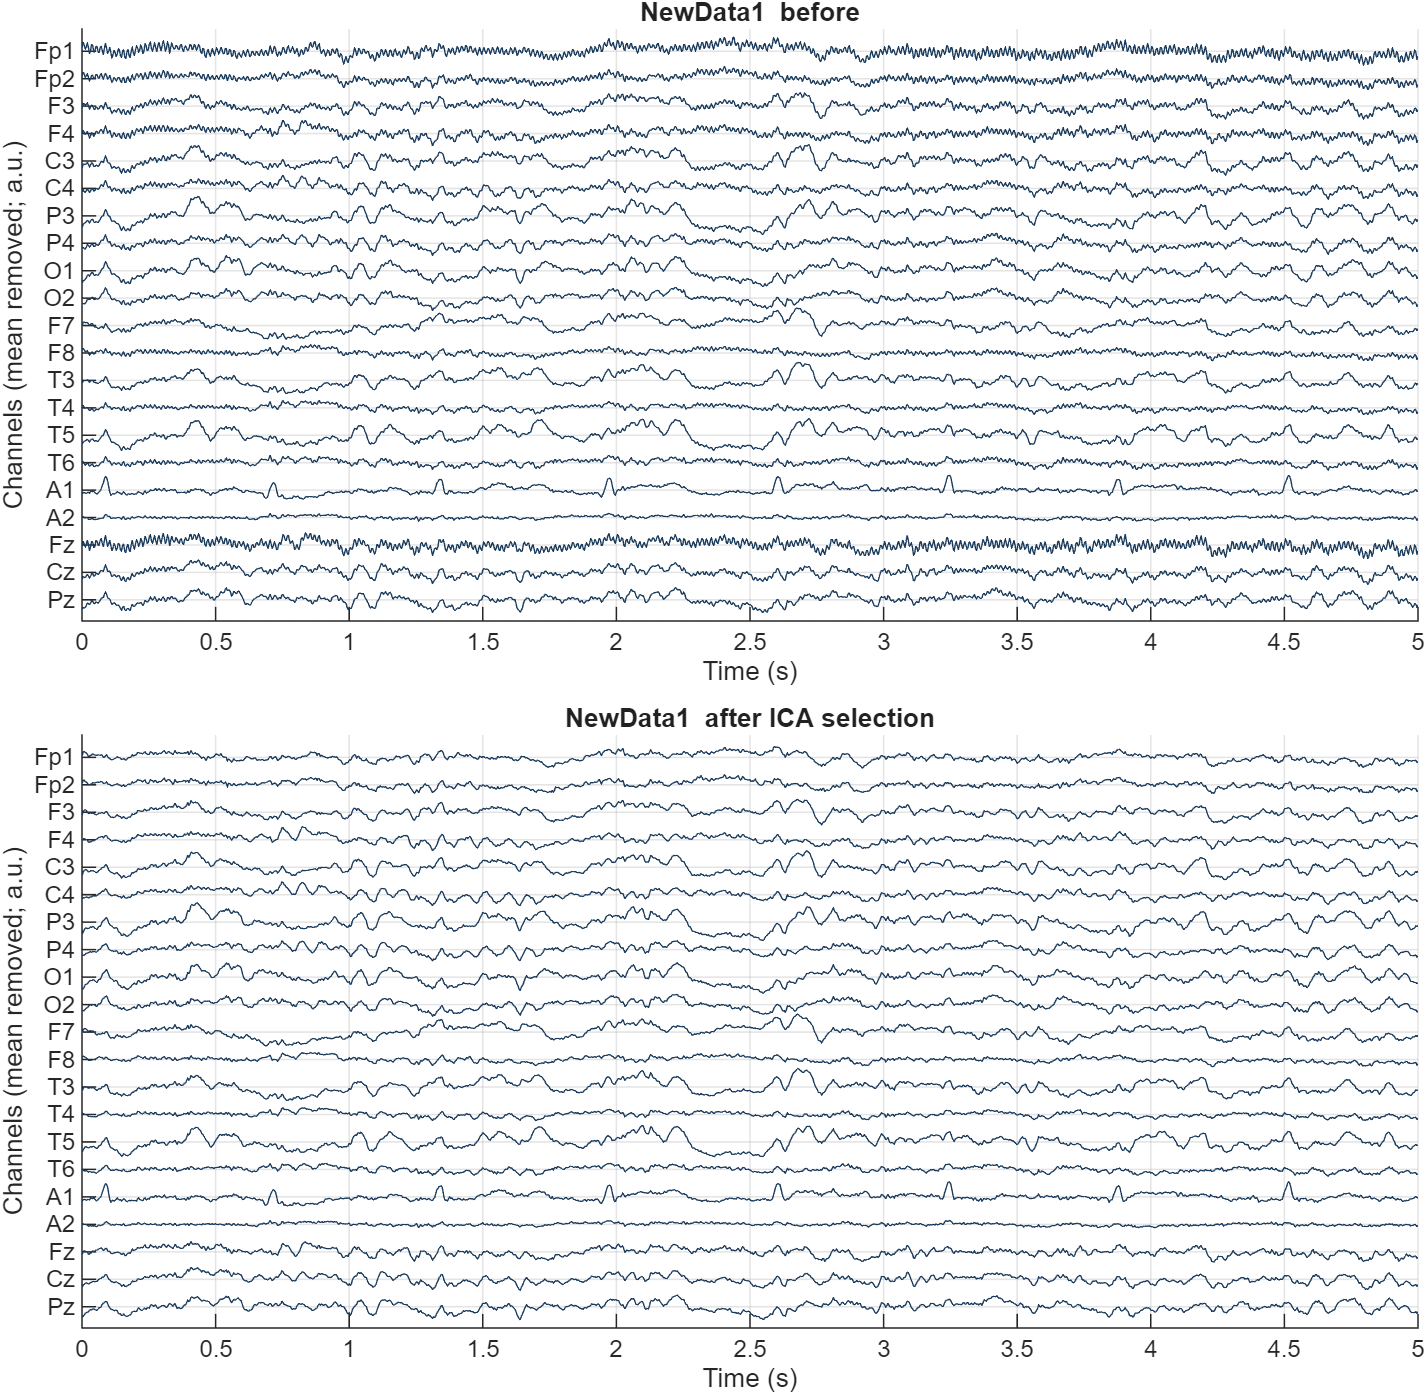
\includegraphics[width=0.85\textwidth,height=0.72\textheight,keepaspectratio]{fig10_newdata1_before_after.png}
\caption{All channels of NewData1 before and after removing IC4; the display is mean-removed and the scale of the two panels is common.}
\label{fig:nd1}
\end{figure}

\subsection*{Selection of components in NewData1}
\subsection*{Questions 3 and 4: Separation and examination of each component}
\begin{taskbox}
\textbf{3.} Apply an ICA algorithm to the signal and obtain the independent components and the mixing matrix. You can use the function \texttt{R2COM.m} (the R2Com algorithm).\\
\textbf{4.} Plot the temporal, spectral and spatial characteristic of each component and decide whether it is desirable or undesirable. To plot the spectral and spatial characteristics you can use \texttt{pwelch.m} (the MATLAB function) and \texttt{plottopomap.m}, respectively. Note: for the temporal and spectral characteristics use the rows of the source matrix, and for the spatial characteristic consider the corresponding columns of the mixing matrix.
\end{taskbox}

COM2R was run with rank 21; $A$ and $W$ have size $21\times21$ and $S$ has size $21\times1251$. For each component, the time series and the PSD were drawn from the corresponding row of $S$, and the spatial map from the corresponding column of $A$. The sheets of all 21 components are given in Figures~26 to~28, and the table of decisions in Appendix~B. Using the column of $W$ instead of the column of $A$ to interpret the sensor propagation pattern is not correct.

IC4 was removed because of the coincidence of three pieces of evidence: a continuous oscillation, a narrow 60~Hz peak and a fixed mixing pattern. In contrast, IC7 has almost periodic events and an appearance similar to cardiac contamination, but it was not removed, because of the absence of an ECG reference and the possibility of ambiguous interpretation in epileptic EEG. Keeping it does not prove that it is brain activity or that it is clean; it is merely a conservative decision.

\subsection*{Question 5: Recording the desired sources and the reconstruction}
\begin{taskbox}
Store the indices of all desired sources in a vector \texttt{SelSources} and reconstruct the denoised signal: $X_{\mathrm{denoised}}=A(:,\mathrm{SelSources})\times S(\mathrm{SelSources},:)$.
\end{taskbox}

\begin{lstlisting}[language=Matlab]
RejectedSources = 4;
SelSources = [1 2 3 5 6 7 8 9 10 11 12 13 14 15 16 17 18 19 20 21];
X_den = A(:,SelSources)*S(SelSources,:) + channelMean;
\end{lstlisting}

By removing one component, the contribution of the remaining 20 components was returned to the sensor space. The ICA method is suitable for this pattern, because the interference has a distinct time course and an approximately constant spatial pattern. This result is not a claim of removing all types of artifacts of this recording.

\subsection*{Question 6: Evaluation before and after}
\begin{taskbox}
Plot the denoised signal and compare it with the original signal. Did you select the correct sources? Was the noise removal performed well? Should step (5) be repeated more carefully?
\end{taskbox}

\begin{equation}
r=\frac{\|X-X_{\mathrm{den}}\|_F^{2}}{\|X-\mu\mathbf{1}^{T}\|_F^{2}}
\end{equation}

\begin{center}
\small
\begin{tabularx}{\textwidth}{@{}>{\raggedright\arraybackslash}Xc>{\raggedright\arraybackslash}X@{}}
\toprule
\textbf{Index} & \textbf{Result} & \textbf{Interpretation}\\
\midrule
Energy ratio of the removed contribution & 0.080883 & The removed share relative to the mean-removed input energy\\
Reduction of the 30--100~Hz power & 5.7978 dB & Attenuation of the high-frequency activity\\
Reduction of the 0.5--4~Hz power & $-0.01986$ dB & A very small and slightly increasing change\\
Median channel correlation & 0.963993 & Relative similarity before and after; there is no clean reference\\
\bottomrule
\end{tabularx}
\end{center}

The energy ratio 0.080883 is not equivalent to ``8.09 percent of the total noise''; it describes the share of the one removed component. Likewise, a high correlation does not prove the validity of the reconstruction relative to a clean EEG. The very small increase in the low-band power is consistent with the fact that the cross-term of the sources in the sensor space is not necessarily non-negative, and it is not necessarily a computational error.

\paragraph{Time and spectral comparison of NewData1.}

\begin{figure}[H]
\centering
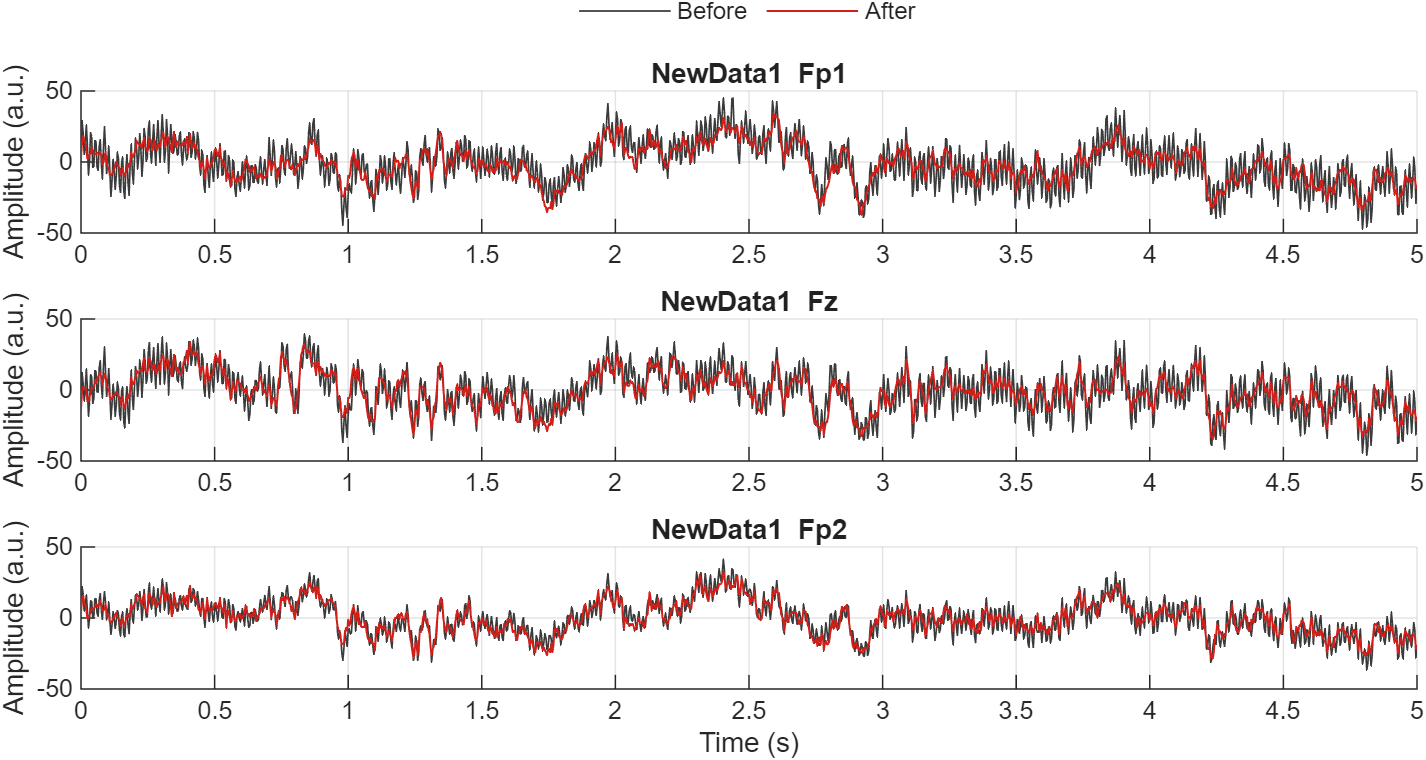
\includegraphics[width=0.9\textwidth]{fig11_newdata1_top_channels.png}
\caption{The channels with the largest RMS of the removed contribution; the fast oscillation is attenuated, but other structures remain.}
\label{fig:nd1top}
\end{figure}

\begin{figure}[H]
\centering
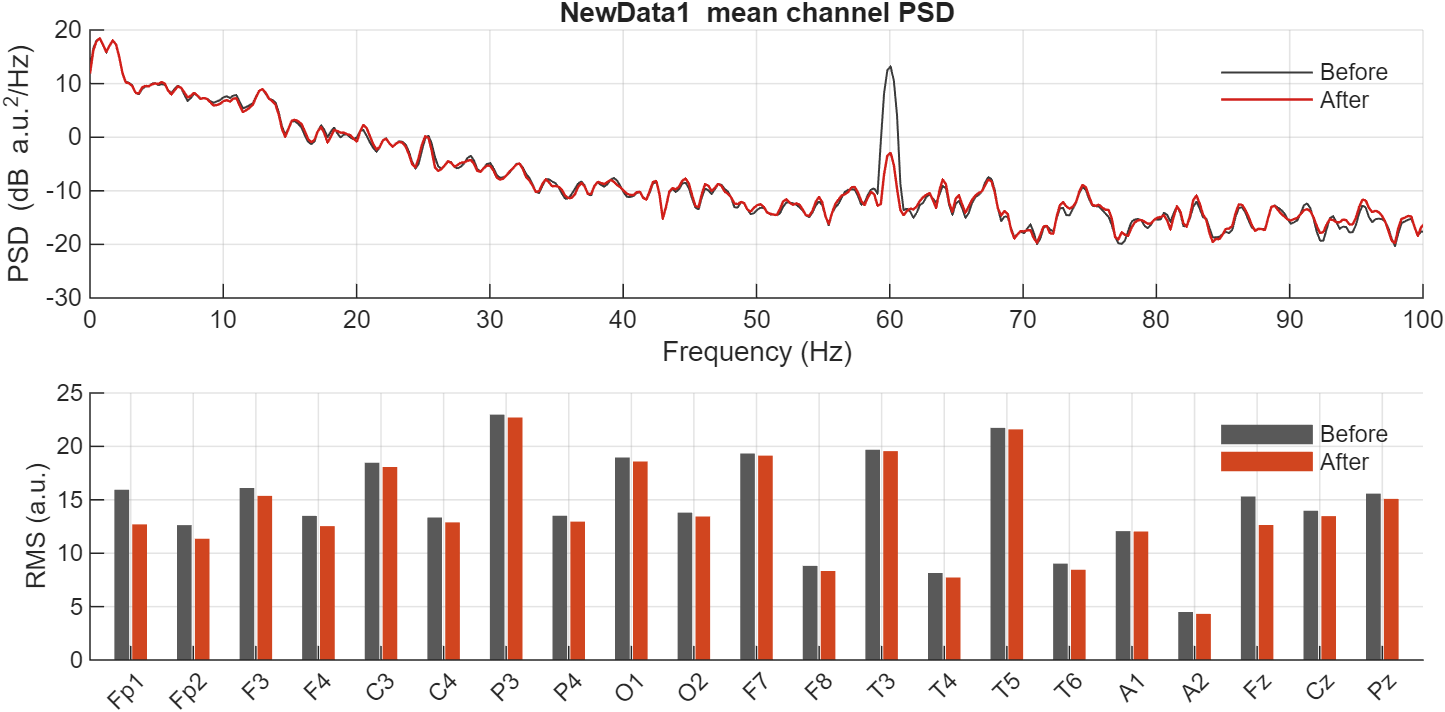
\includegraphics[width=0.9\textwidth]{fig12_newdata1_psd_rms.png}
\caption{Mean PSD and RMS of each channel in NewData1 before and after the removal; a decrease in power does not mean reconstruction accuracy.}
\label{fig:nd1psd}
\end{figure}

The reduction of the peak near 60~Hz, together with the preservation of the major part of the temporal structure, supports the choice of IC4. However, the lack of a clean reference and the retention of IC7 do not allow a claim of complete cleaning. A later review is better carried out with an ECG reference channel or a longer recording, not by the automatic removal of more components.

\section{Part 2: Examination of the Real Data NewData3}

\begin{taskbox}[Tasks]
The same steps as for NewData1 (Questions 1 to 6 of the previous section) are carried out for the second selected recording.
\end{taskbox}

\subsection*{Questions 1 and 2: Observation and identification of the artifact pattern}

The NewData3 recording also has 21 channels and the interval from zero to five seconds. Three slow transients with a large amplitude are seen in the frontal channels at about one, two and a half, and four and a half seconds. There is also localized fast activity in T4. Through the ICA examination, these two patterns led to two independent sets of evidence; large amplitude alone was not made the basis of removal.

\begin{figure}[H]
\centering
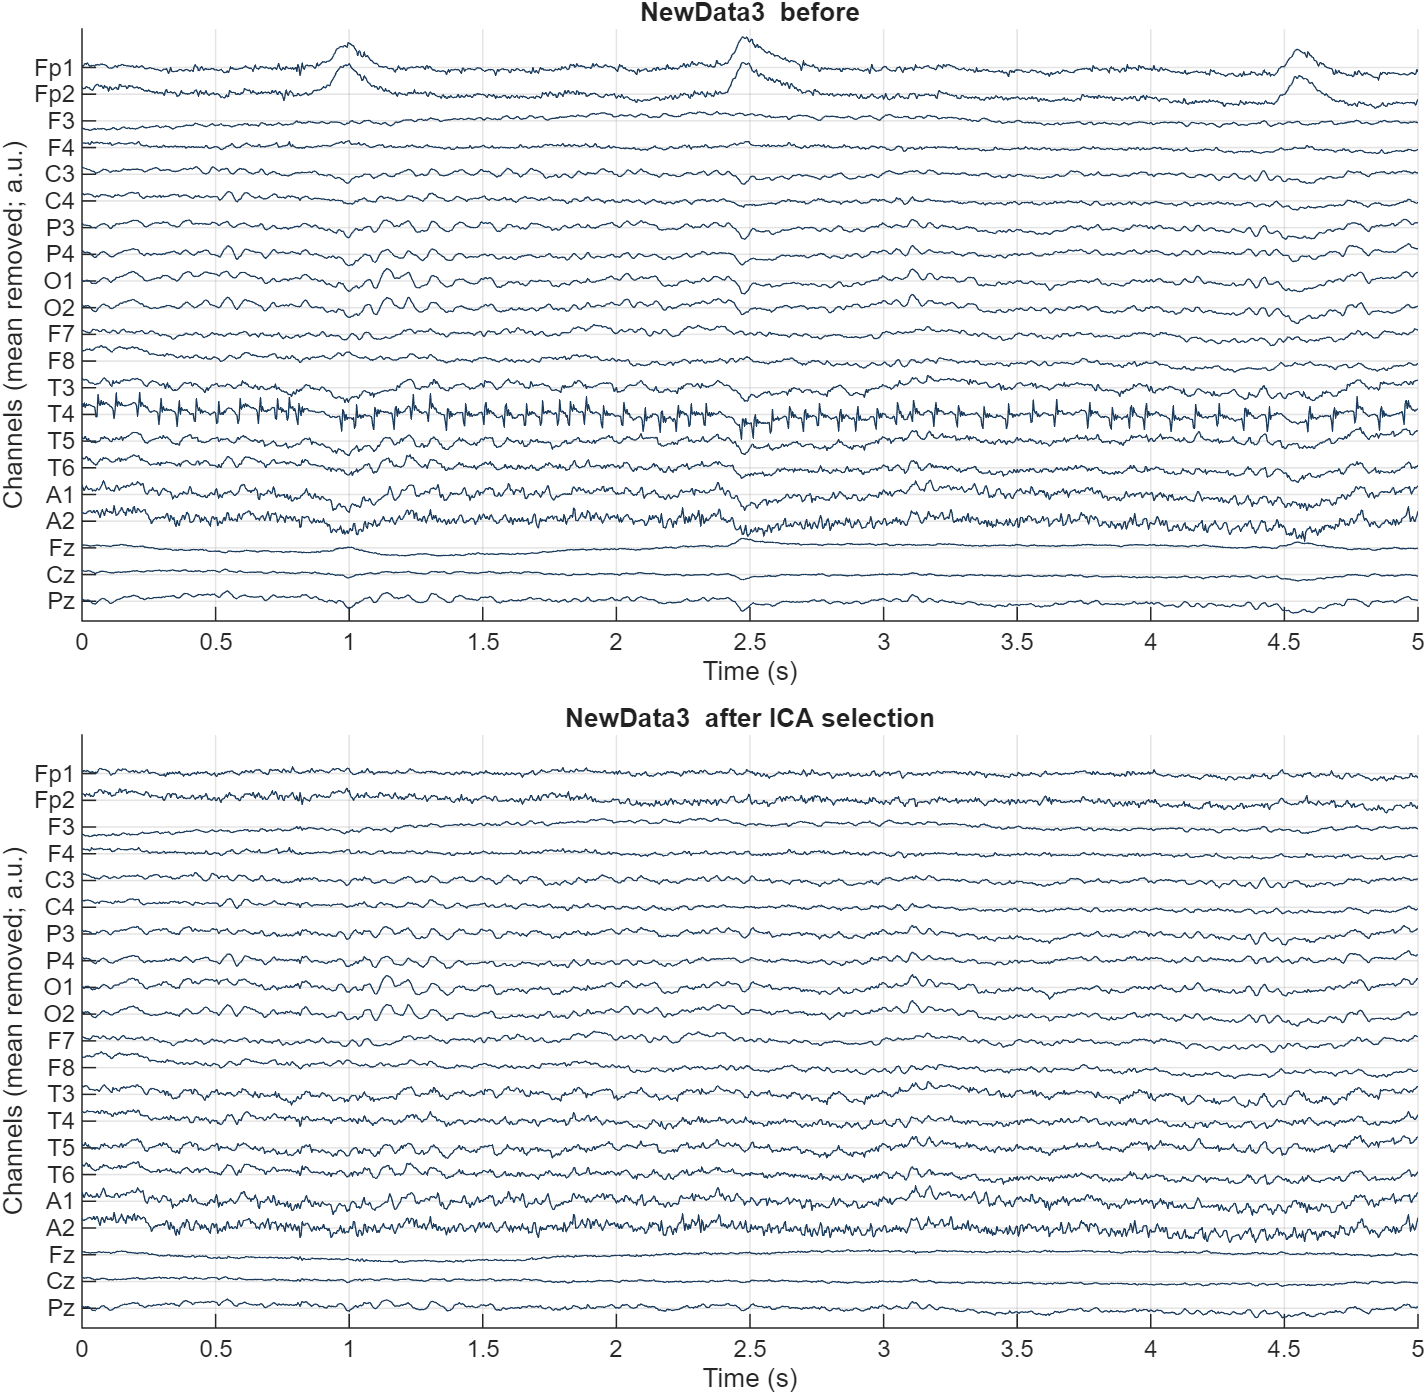
\includegraphics[width=0.85\textwidth,height=0.72\textheight,keepaspectratio]{fig13_newdata3_before_after.png}
\caption{All channels of NewData3 before and after removing IC1 and IC8; common scale, showing the reduction of the frontal transients and of the T4 contamination.}
\label{fig:nd3}
\end{figure}

\subsection*{Selection of components in NewData3}
\subsection*{Questions 3 and 4: Separation and evidence for the components}

The numerical rank was 21, and $A$ and $W$ of size $21\times21$ and $S$ of size $21\times1251$ were obtained. Figures~29 to~31 show the time course, the PSD and the spatial pattern of all components. The two components below had the clearer evidence for tentative removal.

\begin{center}
\begin{tabularx}{\textwidth}{@{}c>{\raggedright\arraybackslash}X>{\raggedright\arraybackslash}X>{\raggedright\arraybackslash}X@{}}
\toprule
\textbf{Component} & \textbf{Temporal and spectral evidence} & \textbf{Spatial evidence} & \textbf{Decision}\\
\midrule
IC1 & Three slow transients; LF $\approx 0.816$ & Frontal share $\approx 0.640$ & Removed as probable blink-like\\
IC8 & HF $\approx 0.805$; lag1 $\approx 0.071$ & Squared-weight concentration $\approx 0.971$ on T4 & Removed as localized high-frequency contamination\\
\bottomrule
\end{tabularx}
\end{center}

In IC1, the coincidence of slow transients, the dominance of low power and a bilateral frontal propagation is consistent with a probable eye blink. In IC8, a broad high-frequency spectrum, a low correlation of adjacent samples and a very strong concentration in T4 support a localized contamination. The peak of IC8 at about 65.4~Hz does not mean a narrow-band linear 65~Hz interference; its spectrum is broad. The exact electrode or muscle origin cannot be determined without independent evidence.

Ambiguous components, including IC14, IC20 and IC21, which have a higher high-frequency share, were kept. In particular, an HF of about 0.619 in IC21 raises the possibility of residual noise, but the spatial dispersion and the absence of specific evidence prevented its definite removal. In epileptic data, a high HF or a sharp event alone is not a sufficient basis for removal.

\subsection*{Question 5: Desired sources and the reconstruction}

\begin{lstlisting}[language=Matlab]
RejectedSources = [1 8];
SelSources = [2 3 4 5 6 7 9 10 11 12 13 14 15 16 17 18 19 20 21];
X_den = A(:,SelSources)*S(SelSources,:) + channelMean;
\end{lstlisting}

In this recording, the back-mapping was carried out with the 19 remaining components. The removal of the two components was justified by two distinct sets of temporal, spectral and spatial evidence; the number of removals is not in itself a quality criterion.

The reduction of low power with the removal of the blink-like component, and the reduction of high power with the removal of the T4 contamination, are consistent with each other. However, the energy ratio of 33.53 percent is neither the percentage of real noise removed nor a measure of the clinical information preserved. The selections are defensible with respect to the available evidence, but the possibility of residual contamination exists. Repeating the selection step with more removals, without independent evidence, is not justified.

\subsection*{Question 6: Evaluation of the NewData3 reconstruction}

\begin{figure}[H]
\centering
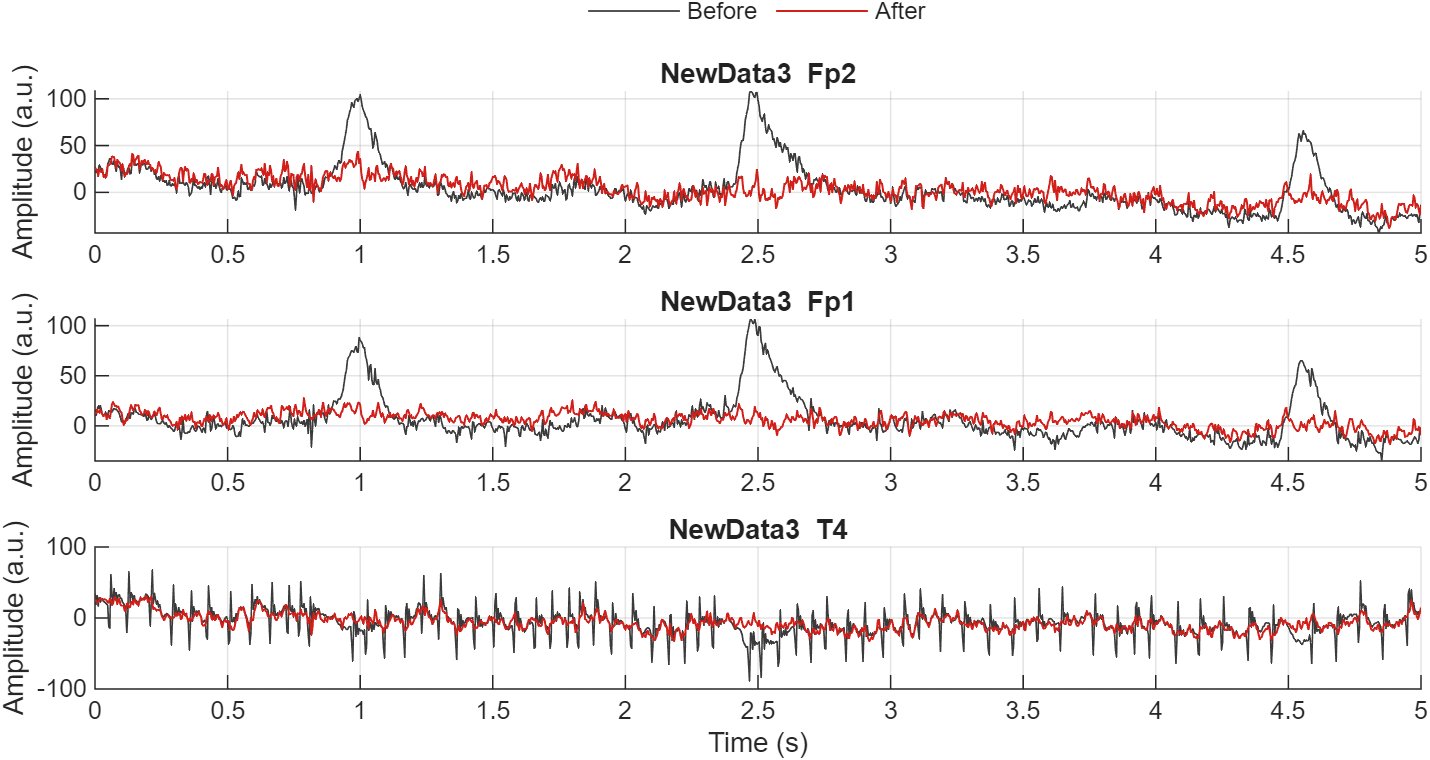
\includegraphics[width=0.9\textwidth]{fig14_newdata3_channels.png}
\caption{Before and after in Fp2, Fp1 and T4; the amplitude of the frontal slow transients and of the localized fast activity has decreased.}
\label{fig:nd3ch}
\end{figure}

\begin{figure}[H]
\centering
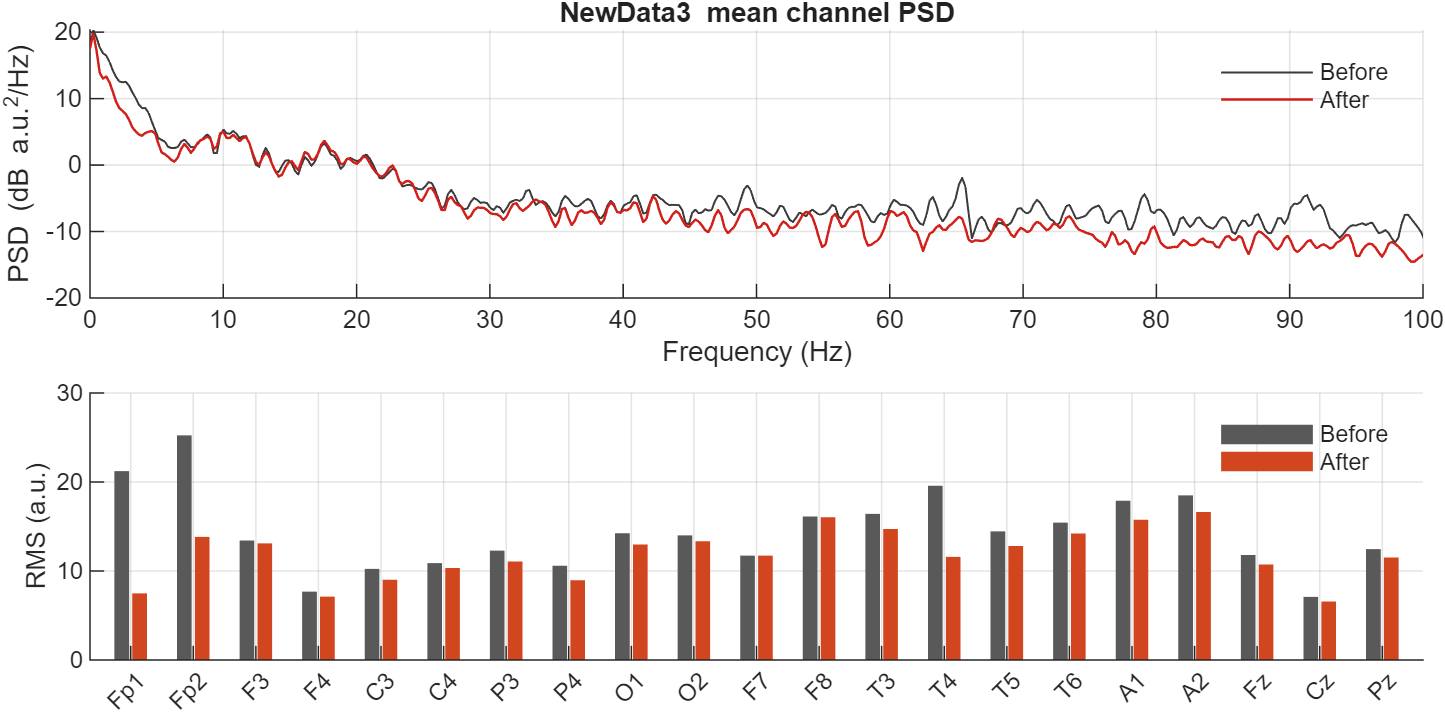
\includegraphics[width=0.9\textwidth]{fig15_newdata3_psd_rms.png}
\caption{Mean PSD and RMS of the channels in NewData3; the simultaneous reduction of low and high power is consistent with the two removed components.}
\label{fig:nd3psd}
\end{figure}

\begin{center}
\begin{tabular}{@{}lc@{}}
\toprule
\textbf{Index} & \textbf{Result}\\
\midrule
Energy ratio of the removed contribution & 0.335279\\
Reduction of the 30--100~Hz power & 2.2695 dB\\
Reduction of the 0.5--4~Hz power & 3.8076 dB\\
Median channel correlation & 0.909780\\
\bottomrule
\end{tabular}
\end{center}

\section{Conclusions and Limitations}

In the simulation part, CoM2 together with the selection of the spiky sources reduced the error relative to the initial observation. At $-5$~dB, both the RRMSE and the temporal shape of the events showed a considerable improvement. At $-15$~dB, despite an SNR improvement of about 8.62~dB, the absolute output error remained large and some spikes were not recovered correctly. The result of this case should therefore be recorded as a limitation of the method and of the source selection, not as a complete cleaning success.

In the real data, an attenuation of the 60~Hz interference in NewData1 and a reduction of the frontal transients and of the T4 contamination in NewData3 were observed. The lack of a clean reference, the shortness of the recordings and the ambiguity of the origin of some components limit the scope of the conclusions. The measures of power, RMS, removed energy and correlation only describe the changes. Keeping the ambiguous components is consistent with the conservative principle of the course notes \rc{2}.

For a subsequent evaluation, a longer recording, an EOG or ECG reference, expert review and a sensitivity test of the component selection can be useful. Examining other ICA algorithms or auxiliary classifiers such as ICLabel is also a path for further development, but there is no result from running them in this experiment \rc{5}. The accuracy of epilepsy detection, the sensitivity of spike detection and the preservation of ERPs were not measured.

\subsection*{Reproduction and checking of the computations}

The code was run with MATLAB R2025b and the Signal Processing Toolbox. The file \texttt{START\_HW2} starts the complete run, and the results, matrices, decision table and figures are saved in the \texttt{results} folder. In the main run, 33 figures were produced in PNG and FIG formats, and 352 checks of numerical consistency and of the existence of the outputs were carried out successfully. The figures of this report were redrawn from the same numerical outputs, with the dimensions adjusted for printing; the data or the selection of the components were not changed in preparing the report.

These checks include the applied SNR, the reconstruction with all components, the mapping of the selected components, the consistency of the tables and the finiteness of the data. Passing them is not a guarantee of the correct identification of all artifacts or of the biological independence of the components. The residual of the full reconstruction in the two real recordings was approximately $1.52\times10^{-15}$ and $1.03\times10^{-15}$.

\clearpage
\section*{Appendix A: Key Code and Organization of the Run}
\addcontentsline{toc}{section}{Appendix A: Key Code and Organization of the Run}

\begin{center}
\begin{tabularx}{\textwidth}{@{}>{\ttfamily}l>{\raggedright\arraybackslash}X@{}}
\toprule
\textnormal{\textbf{File}} & \textbf{Role}\\
\midrule
START\_HW2.m & Running the complete computations and checking the outputs\\
prepare\_hw2.m & Loading, building the observation, mean removal and running COM2R\\
hw2\_features.m & PSD and the temporal and spatial features\\
run\_hw2.m & Component selection, reconstruction, computing the metrics and drawing the figures\\
hw2\_topomap.m & Polar electrode map with the color of the true weight\\
validate\_hw2.m & Independent check of the numerical consistency and of the output files\\
\bottomrule
\end{tabularx}
\end{center}

\subsection*{Core code of the simulation}

\begin{lstlisting}[language=Matlab]
sigma = norm(X_org,'fro')/norm(X_noise,'fro') ...
        * 10^(-targetSNR/20);
X = X_org + sigma*X_noise;
channelMean = mean(X,2);
Xc = X-channelMean;
[A,W,sweeps] = COM2R(Xc,size(X,1));
S = W*Xc;
% The actual implementation obtains these from hw2_features.
SelSources = find(excessKurtosis >= 6 & peakZ >= 6 & HF <= .20);
X_den = A(:,SelSources)*S(SelSources,:) + channelMean;
RRMSE = norm(X_org-X_den,'fro')/norm(X_org,'fro');
SNRout = -20*log10(RRMSE);
\end{lstlisting}

\subsection*{Computing the PSD and reconstructing the real data}

\begin{lstlisting}[language=Matlab]
[P,f] = pwelch((S-mean(S,2))',hamming(500),250,1024,250);
RejectedSources = [1 8]; % NewData3 only
SelSources = setdiff(1:size(S,1),RejectedSources);
X_den = A(:,SelSources)*S(SelSources,:) + channelMean;
\end{lstlisting}

The component numbers are valid only for the current data and the current method. After a change of the preprocessing, the rank or the version of the algorithm, the selections must be reviewed again. For a complete rerun, \texttt{START\_HW2} is executed; using the stored ICA results is appropriate only when the data and the decomposition settings have not changed.

\clearpage
\section*{Appendix B: Component Decision Table}
\addcontentsline{toc}{section}{Appendix B: Component Decision Table}

In the real-data tables, ``Keep'' means that there is not sufficient evidence for removal; it does not prove the cleanliness or the brain origin of the component. HF and LF are ratios; to convert them to percentages they must be multiplied by one hundred. The numbers were taken from the same CSV files of the final run.

\subsection*{Decisions of NewData1}
\begin{center}
\small
\begin{longtable}{@{}cccccp{6.4cm}@{}}
\toprule
\textbf{IC} & \textbf{HF} & \textbf{LF} & $\kappa$ & \textbf{Decision} & \textbf{Evidence and consideration}\\
\midrule
\endhead
1 & 0.061 & 0.346 & 2.56 & Keep & Low HF and non-intense spatial concentration\\
2 & 0.061 & 0.433 & 3.19 & Keep & Slowness without a specific ocular pattern\\
3 & 0.023 & 0.349 & 1.90 & Keep & Frontal location alone is not sufficient\\
4 & 0.768 & 0.057 & -0.82 & \textcolor{accent}{\textbf{Remove}} & Continuous oscillation and a narrow peak near 60~Hz\\
5 & 0.043 & 0.336 & 7.06 & Keep & Sharp transient with low HF\\
6 & 0.054 & 0.473 & -0.50 & Keep & Relative slowness without sufficient evidence for removal\\
7 & 0.070 & 0.114 & 8.41 & Keep & Probably ECG-like; kept for review\\
8 & 0.041 & 0.473 & -0.46 & Keep & Low power and a relatively diffuse map\\
9 & 0.043 & 0.499 & -0.60 & Keep & Slowness alone is not a criterion for removal\\
10 & 0.050 & 0.457 & -0.18 & Keep & Low HF and a diffuse map\\
11 & 0.033 & 0.397 & -0.28 & Keep & Frontal share without sufficient temporal evidence\\
12 & 0.115 & 0.546 & 4.01 & Keep & Slowness with a low frontal share\\
13 & 0.115 & 0.358 & 5.10 & Keep & A sharp transient alone is not sufficient\\
14 & 0.058 & 0.328 & -0.68 & Keep & Low HF and no specific evidence\\
15 & 0.036 & 0.326 & 8.66 & Keep & High kurtosis with a very low HF\\
16 & 0.051 & 0.295 & 2.83 & Keep & Moderate concentration without complementary evidence\\
17 & 0.036 & 0.372 & 5.72 & Keep & Frontal propagation without a specific pattern\\
18 & 0.077 & 0.387 & 3.49 & Keep & Moderate concentration and low HF\\
19 & 0.045 & 0.265 & 1.75 & Keep & Frontal location alone is not a reason for an artifact\\
20 & 0.086 & 0.359 & 5.34 & Keep & Sharp transient with low HF\\
21 & 0.133 & 0.278 & 1.23 & Keep & No resemblance to a clear narrow-band interference\\
\bottomrule
\end{longtable}
\end{center}

\clearpage
\subsection*{Decisions of NewData3}
\begin{center}
\small
\begin{longtable}{@{}cccccp{6.4cm}@{}}
\toprule
\textbf{IC} & \textbf{HF} & \textbf{LF} & $\kappa$ & \textbf{Decision} & \textbf{Evidence and consideration}\\
\midrule
\endhead
1 & 0.042 & 0.816 & 7.04 & \textcolor{accent}{\textbf{Remove}} & Three slow transients and bilateral frontal propagation\\
2 & 0.226 & 0.286 & -0.43 & Keep & Moderate HF and a diffuse map\\
3 & 0.214 & 0.367 & 9.76 & Keep & Early transient of ambiguous origin\\
4 & 0.120 & 0.256 & 2.30 & Keep & Peak at about 12~Hz; no specific evidence\\
5 & 0.360 & 0.228 & -0.32 & Keep & Possible mixing; evidence for removal is not sufficient\\
6 & 0.118 & 0.245 & 5.03 & Keep & Sharp transient with low HF\\
7 & 0.140 & 0.492 & 2.12 & Keep & Moderate slowness without specific evidence\\
8 & 0.805 & 0.010 & 3.48 & \textcolor{accent}{\textbf{Remove}} & Broad HF and a very intense concentration in T4\\
9 & 0.124 & 0.273 & -0.38 & Keep & Low HF and a non-intense concentration\\
10 & 0.078 & 0.291 & 5.37 & Keep & Sharp event with low HF\\
11 & 0.153 & 0.377 & 1.80 & Keep & Frontal share alone is not sufficient\\
12 & 0.077 & 0.506 & -0.78 & Keep & Frontal slowness without a clear blink pattern\\
13 & 0.105 & 0.315 & 4.55 & Keep & Sharp transient without sufficient evidence for removal\\
14 & 0.395 & 0.238 & -0.17 & Keep & Higher HF; probable and ambiguous mixing\\
15 & 0.255 & 0.269 & -0.44 & Keep & Moderate HF and a diffuse map\\
16 & 0.310 & 0.176 & 1.08 & Keep & Possible mixing; no very intense concentration\\
17 & 0.259 & 0.237 & -0.37 & Keep & Moderate HF without independent evidence\\
18 & 0.185 & 0.483 & 2.06 & Keep & Slowness without a clear blink pattern\\
19 & 0.160 & 0.209 & 2.38 & Keep & No specific evidence for removal\\
20 & 0.436 & 0.158 & 2.25 & Keep & Higher HF; kept for review\\
21 & 0.619 & 0.139 & 2.53 & Keep & High HF but ambiguous origin; review needed\\
\bottomrule
\end{longtable}
\end{center}

\clearpage
\subsection*{Decision on the simulation sources at an SNR of $-5$~dB}
A component was kept only when all three conditions on the excess kurtosis, PeakZ and HF hold. This instructional decision must be interpreted together with the temporal and spectral shape and the output error.
\begin{center}
\small
\begin{longtable}{@{}ccccc@{}}
\toprule
\textbf{IC} & \textbf{Excess kurtosis} & \textbf{PeakZ} & \textbf{HF} & \textbf{Decision}\\
\midrule
\endhead
1 & 2.14 & 5.93 & 0.711 & \textcolor{accent}{\textbf{Remove}}\\
2 & 14.69 & 6.73 & 0.025 & Keep\\
3 & 8.53 & 7.87 & 0.746 & \textcolor{accent}{\textbf{Remove}}\\
4 & 2.94 & 6.65 & 0.774 & \textcolor{accent}{\textbf{Remove}}\\
5 & 18.78 & 9.49 & 0.070 & Keep\\
6 & 109.57 & 26.55 & 0.778 & \textcolor{accent}{\textbf{Remove}}\\
7 & 5.57 & 8.47 & 0.707 & \textcolor{accent}{\textbf{Remove}}\\
8 & 8.25 & 8.51 & 0.857 & \textcolor{accent}{\textbf{Remove}}\\
9 & 69.14 & 12.93 & 0.044 & Keep\\
10 & 8.96 & 8.81 & 0.155 & Keep\\
11 & 3.68 & 6.46 & 0.175 & \textcolor{accent}{\textbf{Remove}}\\
12 & 24.95 & 12.17 & 0.065 & Keep\\
13 & 4.37 & 7.44 & 0.738 & \textcolor{accent}{\textbf{Remove}}\\
14 & 4.10 & 10.07 & 0.428 & \textcolor{accent}{\textbf{Remove}}\\
15 & 1.89 & 6.77 & 0.196 & \textcolor{accent}{\textbf{Remove}}\\
16 & 41.08 & 13.83 & 0.807 & \textcolor{accent}{\textbf{Remove}}\\
17 & 59.24 & 18.87 & 0.771 & \textcolor{accent}{\textbf{Remove}}\\
18 & 1.12 & 4.95 & 0.153 & \textcolor{accent}{\textbf{Remove}}\\
19 & 20.41 & 13.51 & 0.456 & \textcolor{accent}{\textbf{Remove}}\\
20 & 3.64 & 7.47 & 0.695 & \textcolor{accent}{\textbf{Remove}}\\
21 & 18.33 & 9.78 & 0.087 & Keep\\
22 & 5.34 & 7.89 & 0.443 & \textcolor{accent}{\textbf{Remove}}\\
23 & 14.05 & 9.45 & 0.114 & Keep\\
24 & 18.87 & 11.26 & 0.763 & \textcolor{accent}{\textbf{Remove}}\\
25 & 1.13 & 6.43 & 0.128 & \textcolor{accent}{\textbf{Remove}}\\
26 & 3.26 & 7.23 & 0.196 & \textcolor{accent}{\textbf{Remove}}\\
27 & 32.01 & 19.15 & 0.581 & \textcolor{accent}{\textbf{Remove}}\\
28 & 28.50 & 15.74 & 0.442 & \textcolor{accent}{\textbf{Remove}}\\
29 & 7.20 & 9.89 & 0.410 & \textcolor{accent}{\textbf{Remove}}\\
30 & 37.82 & 19.85 & 0.560 & \textcolor{accent}{\textbf{Remove}}\\
31 & 0.19 & 5.01 & 0.159 & \textcolor{accent}{\textbf{Remove}}\\
32 & 14.08 & 9.70 & 0.146 & Keep\\
\bottomrule
\end{longtable}
\end{center}

\clearpage
\subsection*{Decision on the simulation sources at an SNR of $-15$~dB}
A component was kept only when all three conditions on the excess kurtosis, PeakZ and HF hold. This instructional decision must be interpreted together with the temporal and spectral shape and the output error.
\begin{center}
\small
\begin{longtable}{@{}ccccc@{}}
\toprule
\textbf{IC} & \textbf{Excess kurtosis} & \textbf{PeakZ} & \textbf{HF} & \textbf{Decision}\\
\midrule
\endhead
1 & 2.21 & 5.83 & 0.726 & \textcolor{accent}{\textbf{Remove}}\\
2 & 9.14 & 7.62 & 0.748 & \textcolor{accent}{\textbf{Remove}}\\
3 & 2.94 & 6.72 & 0.777 & \textcolor{accent}{\textbf{Remove}}\\
4 & 110.85 & 26.41 & 0.785 & \textcolor{accent}{\textbf{Remove}}\\
5 & 8.14 & 8.40 & 0.859 & \textcolor{accent}{\textbf{Remove}}\\
6 & 5.48 & 8.06 & 0.713 & \textcolor{accent}{\textbf{Remove}}\\
7 & 72.51 & 13.10 & 0.043 & Keep\\
8 & 10.44 & 9.18 & 0.167 & Keep\\
9 & 4.18 & 6.27 & 0.167 & \textcolor{accent}{\textbf{Remove}}\\
10 & 4.62 & 10.34 & 0.414 & \textcolor{accent}{\textbf{Remove}}\\
11 & 4.29 & 7.01 & 0.744 & \textcolor{accent}{\textbf{Remove}}\\
12 & 40.80 & 14.05 & 0.806 & \textcolor{accent}{\textbf{Remove}}\\
13 & 20.73 & 13.73 & 0.458 & \textcolor{accent}{\textbf{Remove}}\\
14 & 60.30 & 19.67 & 0.772 & \textcolor{accent}{\textbf{Remove}}\\
15 & 2.77 & 5.14 & 0.149 & \textcolor{accent}{\textbf{Remove}}\\
16 & 5.33 & 7.71 & 0.461 & \textcolor{accent}{\textbf{Remove}}\\
17 & 3.52 & 7.22 & 0.692 & \textcolor{accent}{\textbf{Remove}}\\
18 & 19.56 & 10.10 & 0.083 & Keep\\
19 & 6.41 & 8.88 & 0.256 & \textcolor{accent}{\textbf{Remove}}\\
20 & 14.00 & 9.45 & 0.115 & Keep\\
21 & 19.90 & 11.91 & 0.746 & \textcolor{accent}{\textbf{Remove}}\\
22 & 1.23 & 6.51 & 0.154 & \textcolor{accent}{\textbf{Remove}}\\
23 & 13.35 & 13.28 & 0.576 & \textcolor{accent}{\textbf{Remove}}\\
24 & 0.18 & 3.91 & 0.121 & \textcolor{accent}{\textbf{Remove}}\\
25 & 4.72 & 7.56 & 0.198 & \textcolor{accent}{\textbf{Remove}}\\
26 & 1.49 & 7.88 & 0.236 & \textcolor{accent}{\textbf{Remove}}\\
27 & 50.90 & 22.58 & 0.689 & \textcolor{accent}{\textbf{Remove}}\\
28 & 0.99 & 5.50 & 0.222 & \textcolor{accent}{\textbf{Remove}}\\
29 & 36.42 & 20.01 & 0.564 & \textcolor{accent}{\textbf{Remove}}\\
30 & 13.17 & 9.81 & 0.089 & Keep\\
31 & 43.10 & 16.66 & 0.433 & \textcolor{accent}{\textbf{Remove}}\\
32 & 13.96 & 9.73 & 0.150 & Keep\\
\bottomrule
\end{longtable}
\end{center}

\clearpage
\section*{Appendix C: Sheets of All Components}
\addcontentsline{toc}{section}{Appendix C: Sheets of All Components}

In each row, the first column shows the time course of $S$, the second column the PSD, and the third column the mixing weights, or the map of the corresponding column of $A$. Blue means kept and red means removed. In the real-data maps, the nose points upward and the left side of the person is on the left of the image. The polar coordinates of the electrode file were used so that A1 and A2 are not placed inside the temporal electrodes of the image. The color of the points shows the true value of the weight, and the interpolation outside the convex hull was not extrapolated.

The IC numbers cannot be matched directly between the two simulation decompositions. The scale and the sign of the map of each component must be read with the color bar of that same map. For the simulation data, the weight column is a bar plot, so that the mixing pattern can be examined without an additional geometric assumption.

\begin{figure}[p]
\centering
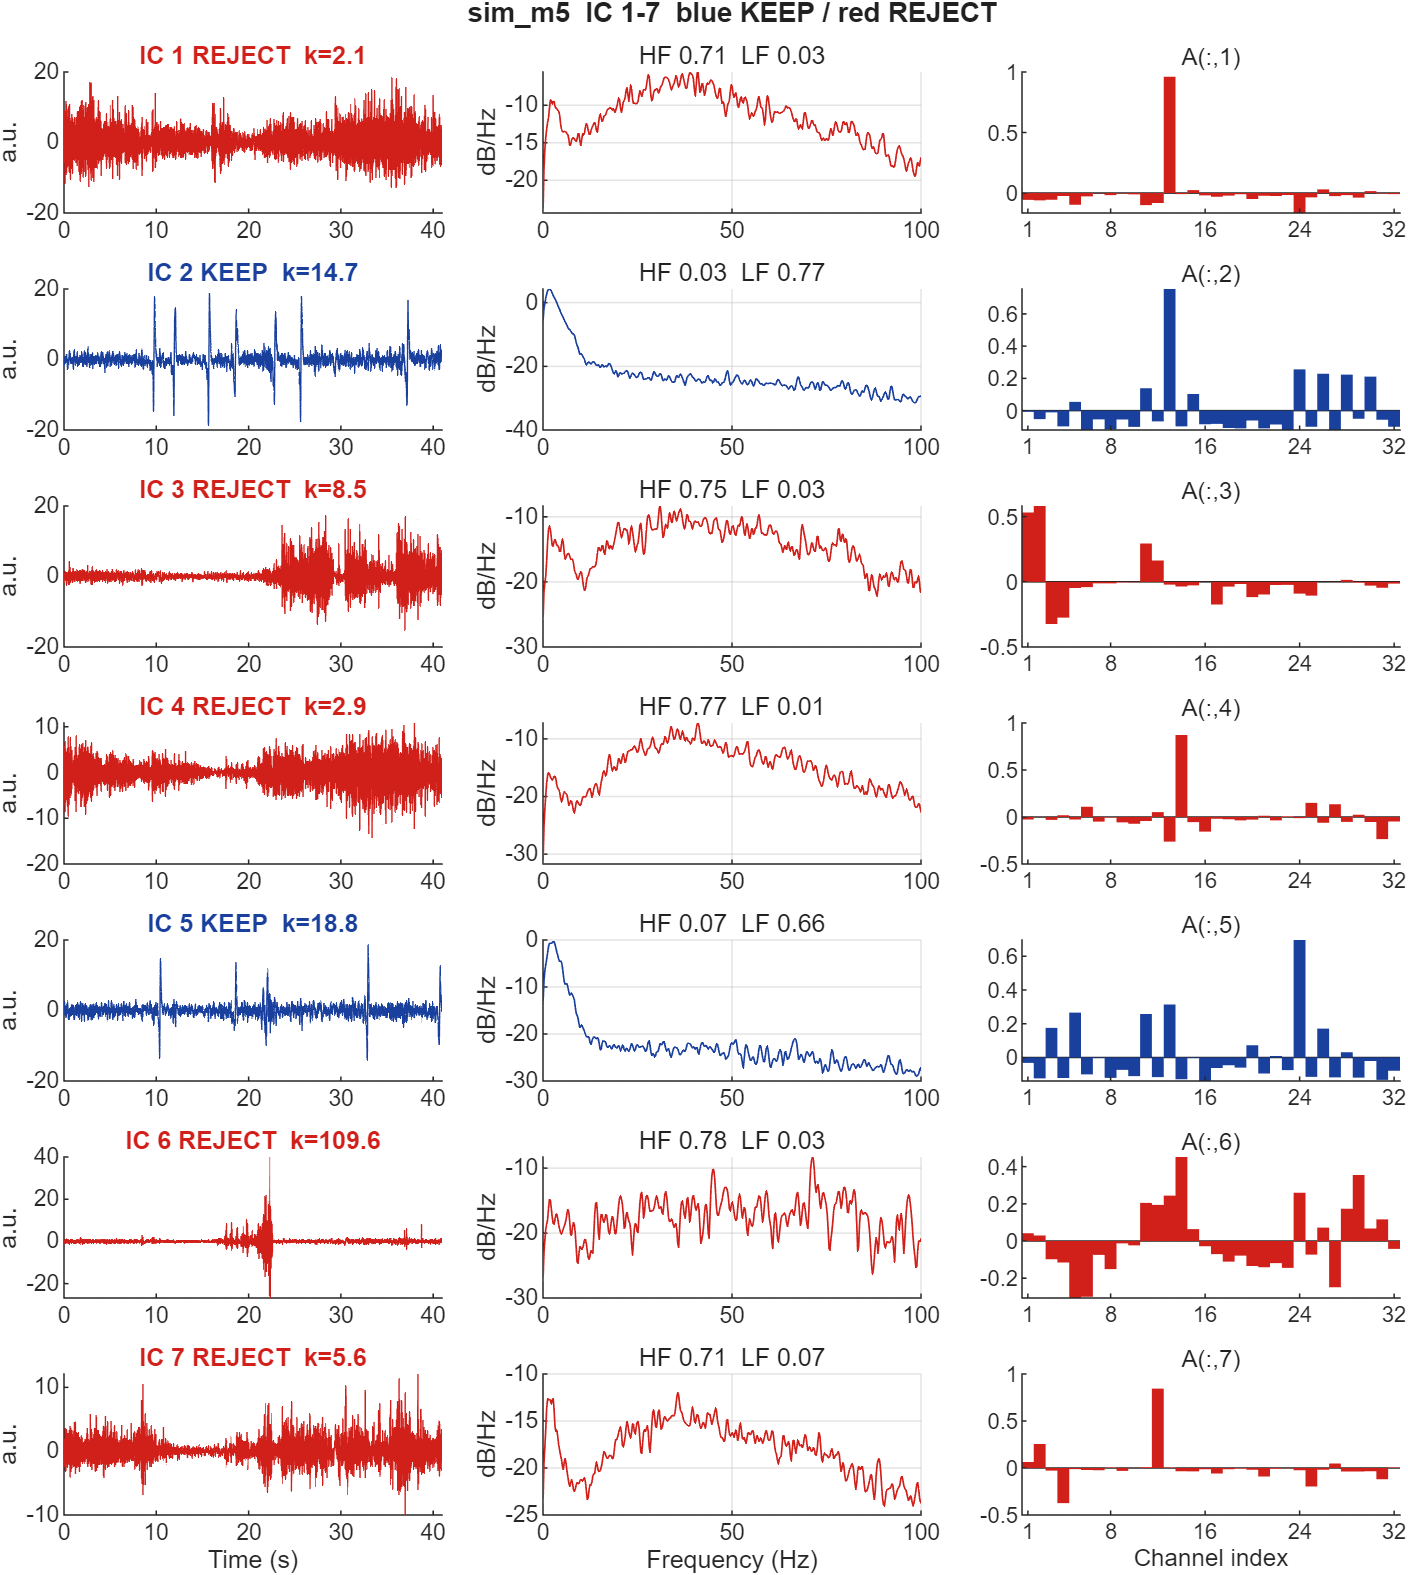
\includegraphics[height=0.80\textheight,width=0.95\textwidth,keepaspectratio]{fig16_sim_m5db_ic01_to_ic07.png}
\caption{Time course, PSD and mixing pattern of components components 1 to 7 in the $-5$~dB simulation.}
\label{fig:app16}
\end{figure}
\begin{figure}[p]
\centering
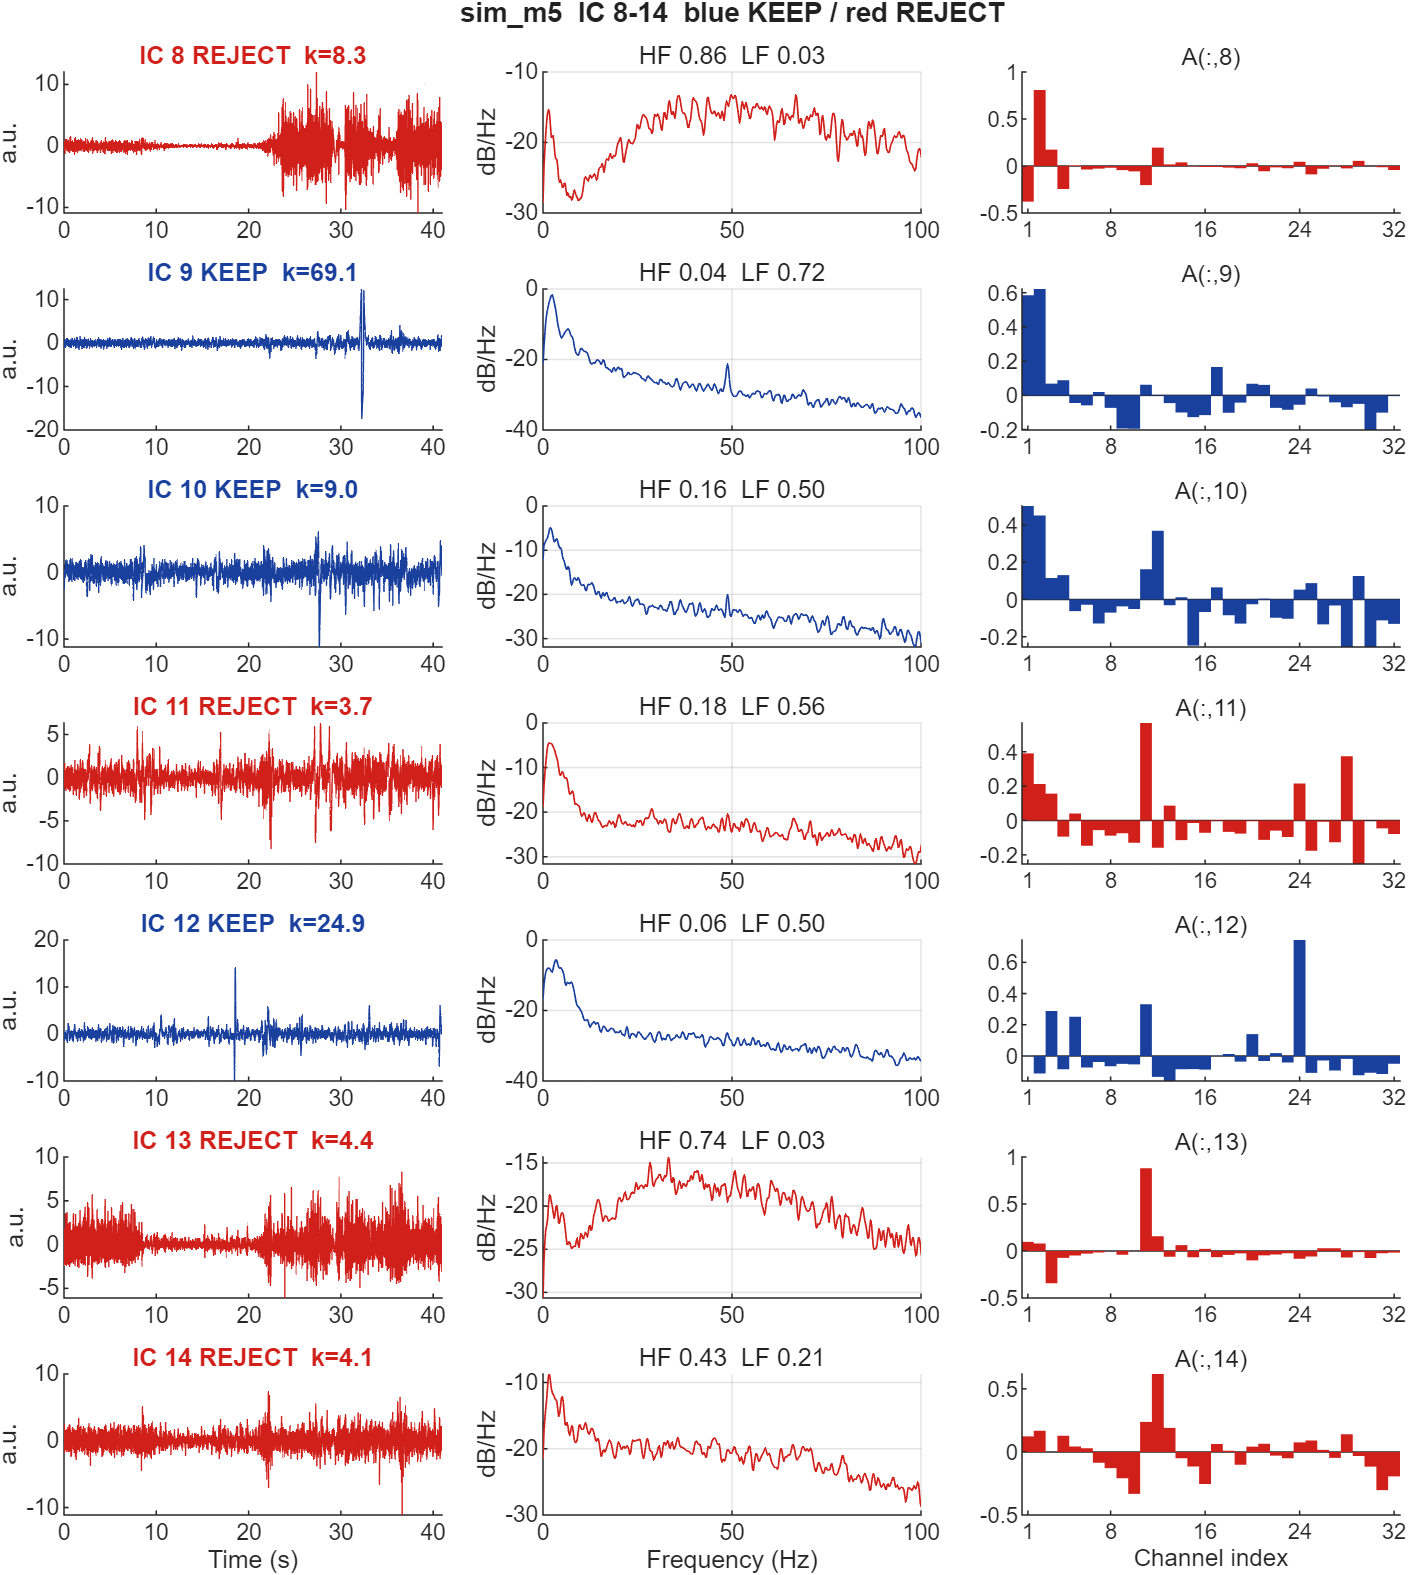
\includegraphics[height=0.80\textheight,width=0.95\textwidth,keepaspectratio]{fig17_sim_m5db_ic08_to_ic14.png}
\caption{Time course, PSD and mixing pattern of components components 8 to 14 in the $-5$~dB simulation.}
\label{fig:app17}
\end{figure}
\begin{figure}[p]
\centering
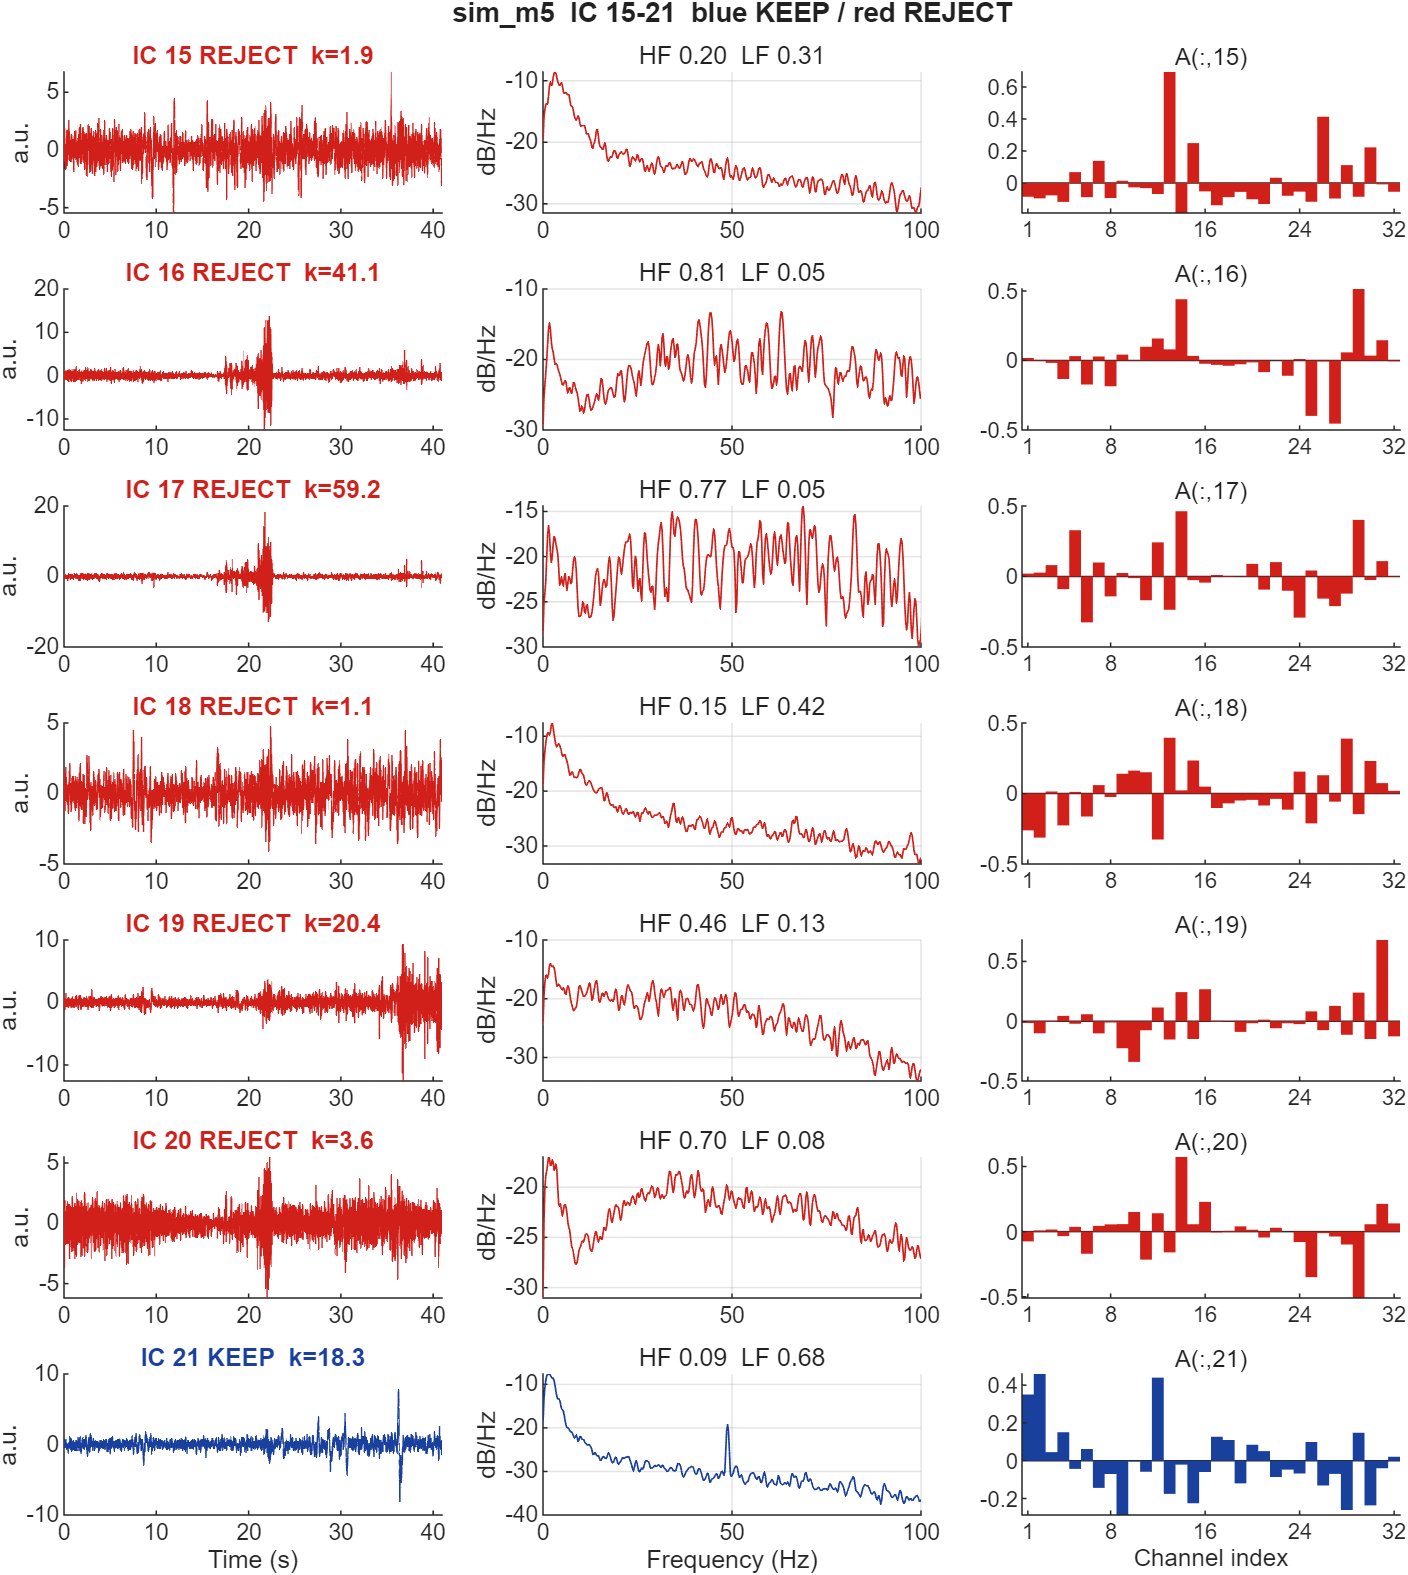
\includegraphics[height=0.80\textheight,width=0.95\textwidth,keepaspectratio]{fig18_sim_m5db_ic15_to_ic21.png}
\caption{Time course, PSD and mixing pattern of components components 15 to 21 in the $-5$~dB simulation.}
\label{fig:app18}
\end{figure}
\begin{figure}[p]
\centering
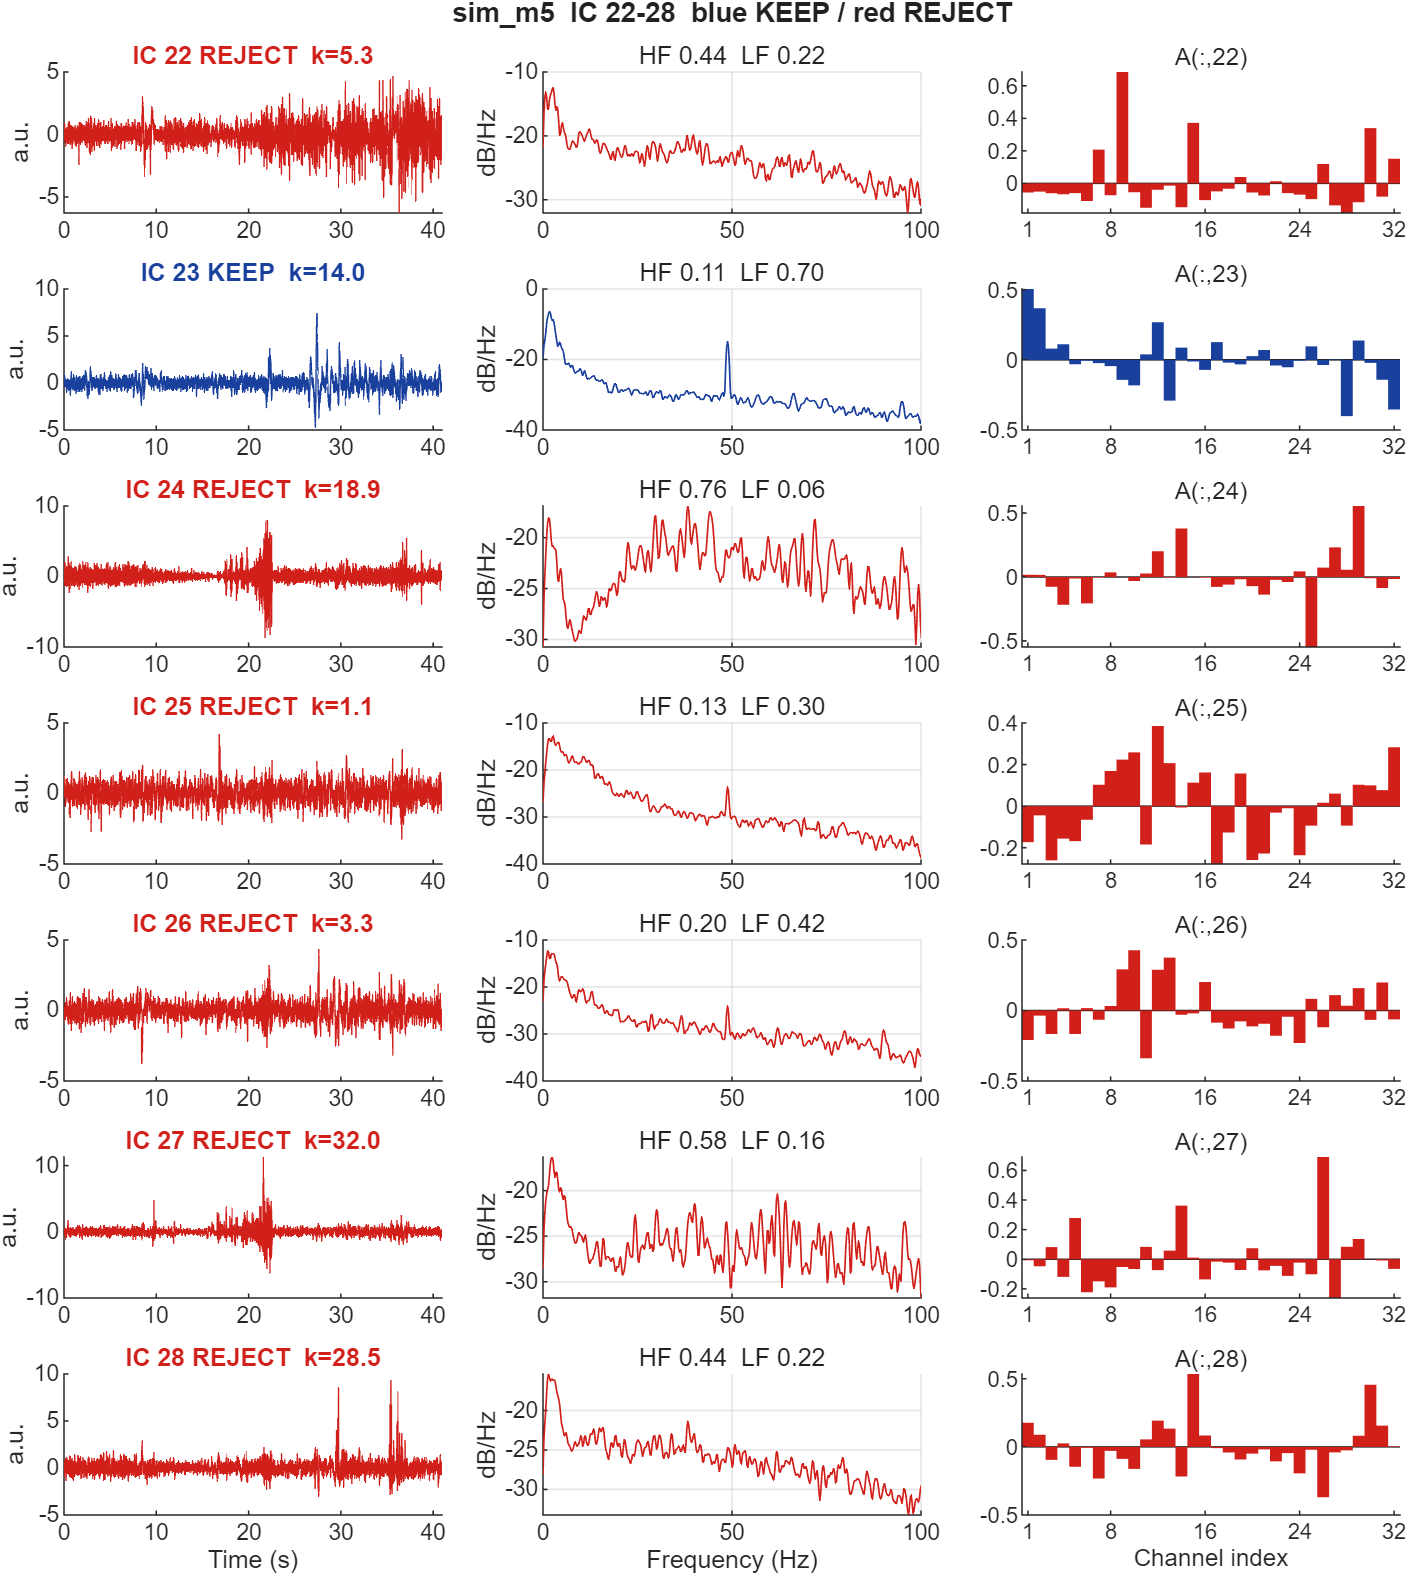
\includegraphics[height=0.80\textheight,width=0.95\textwidth,keepaspectratio]{fig19_sim_m5db_ic22_to_ic28.png}
\caption{Time course, PSD and mixing pattern of components components 22 to 28 in the $-5$~dB simulation.}
\label{fig:app19}
\end{figure}
\begin{figure}[p]
\centering
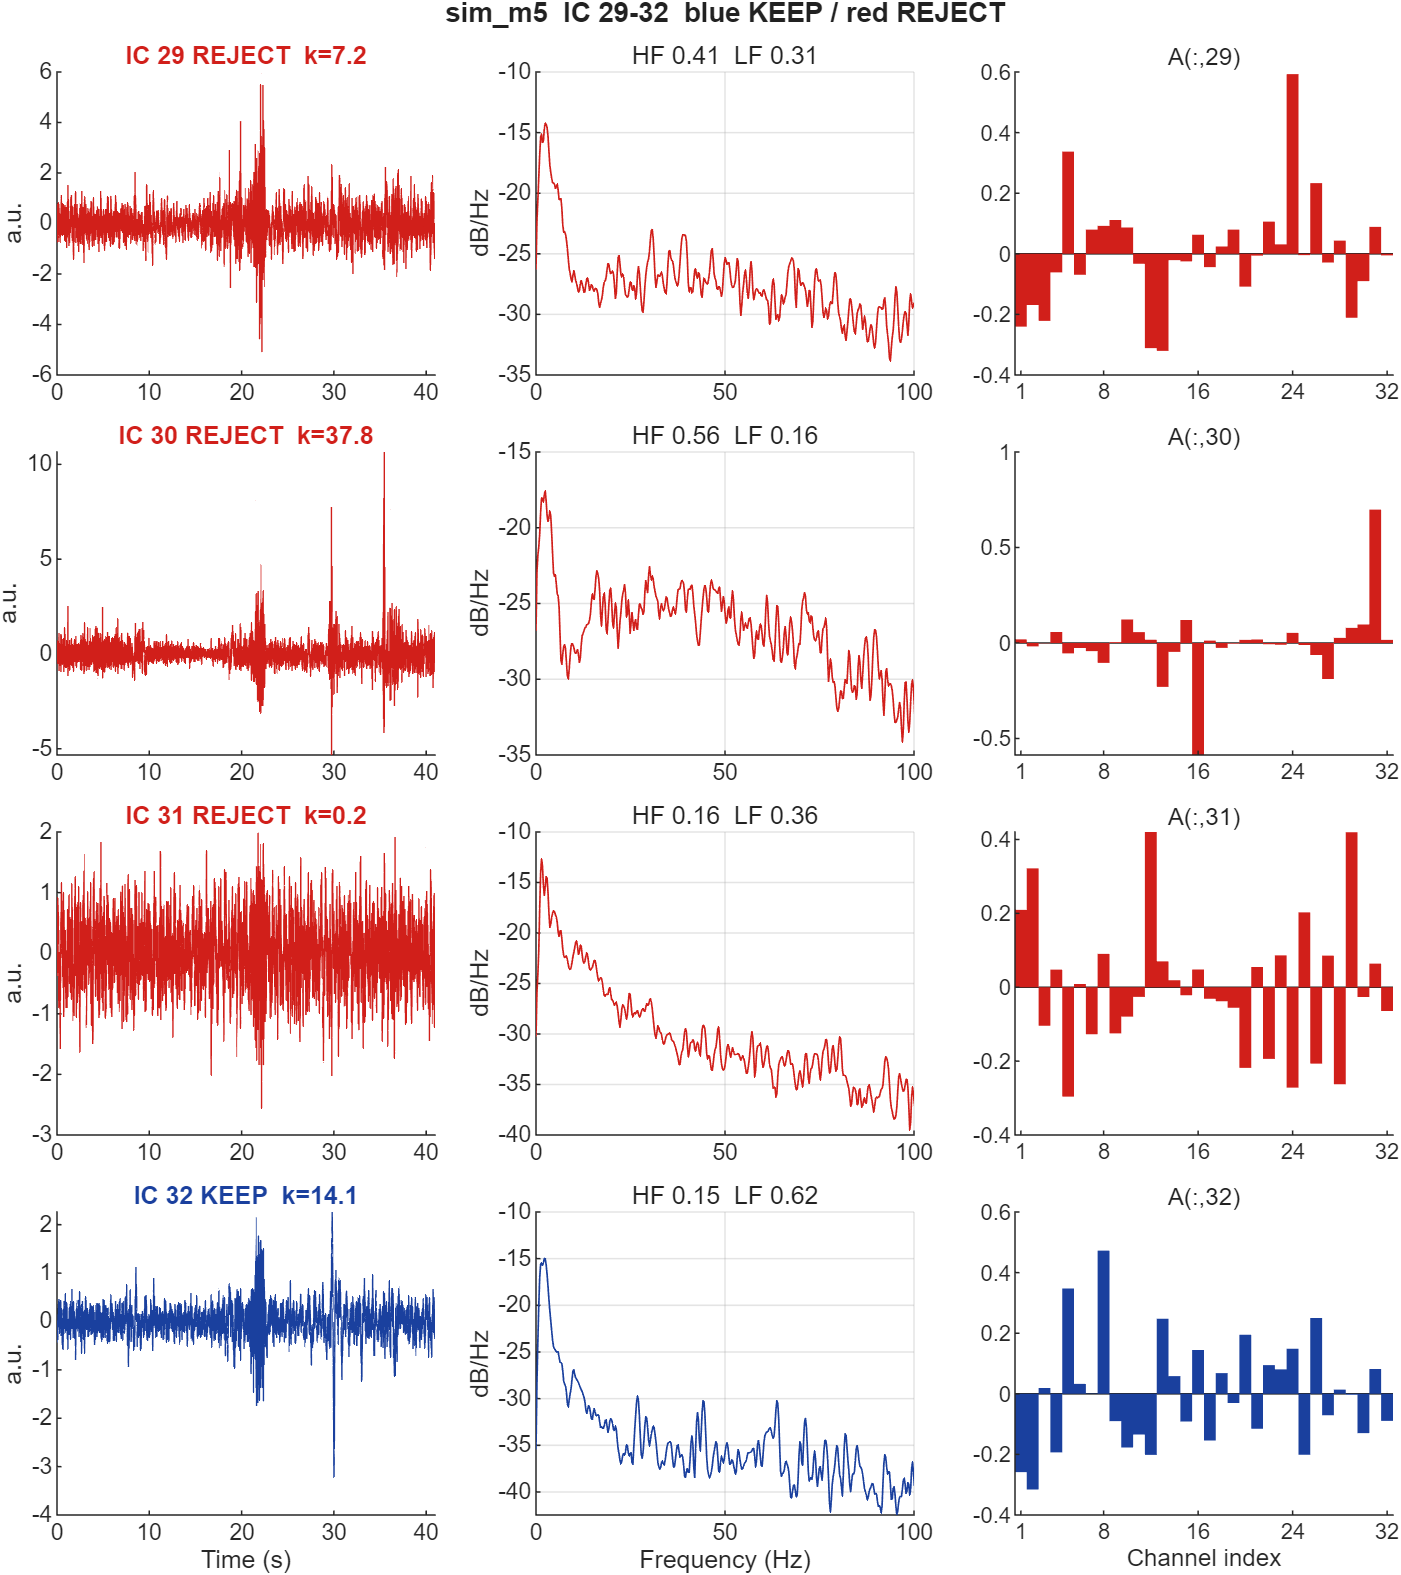
\includegraphics[height=0.80\textheight,width=0.95\textwidth,keepaspectratio]{fig20_sim_m5db_ic29_to_ic32.png}
\caption{Time course, PSD and mixing pattern of components components 29 to 32 in the $-5$~dB simulation.}
\label{fig:app20}
\end{figure}
\begin{figure}[p]
\centering
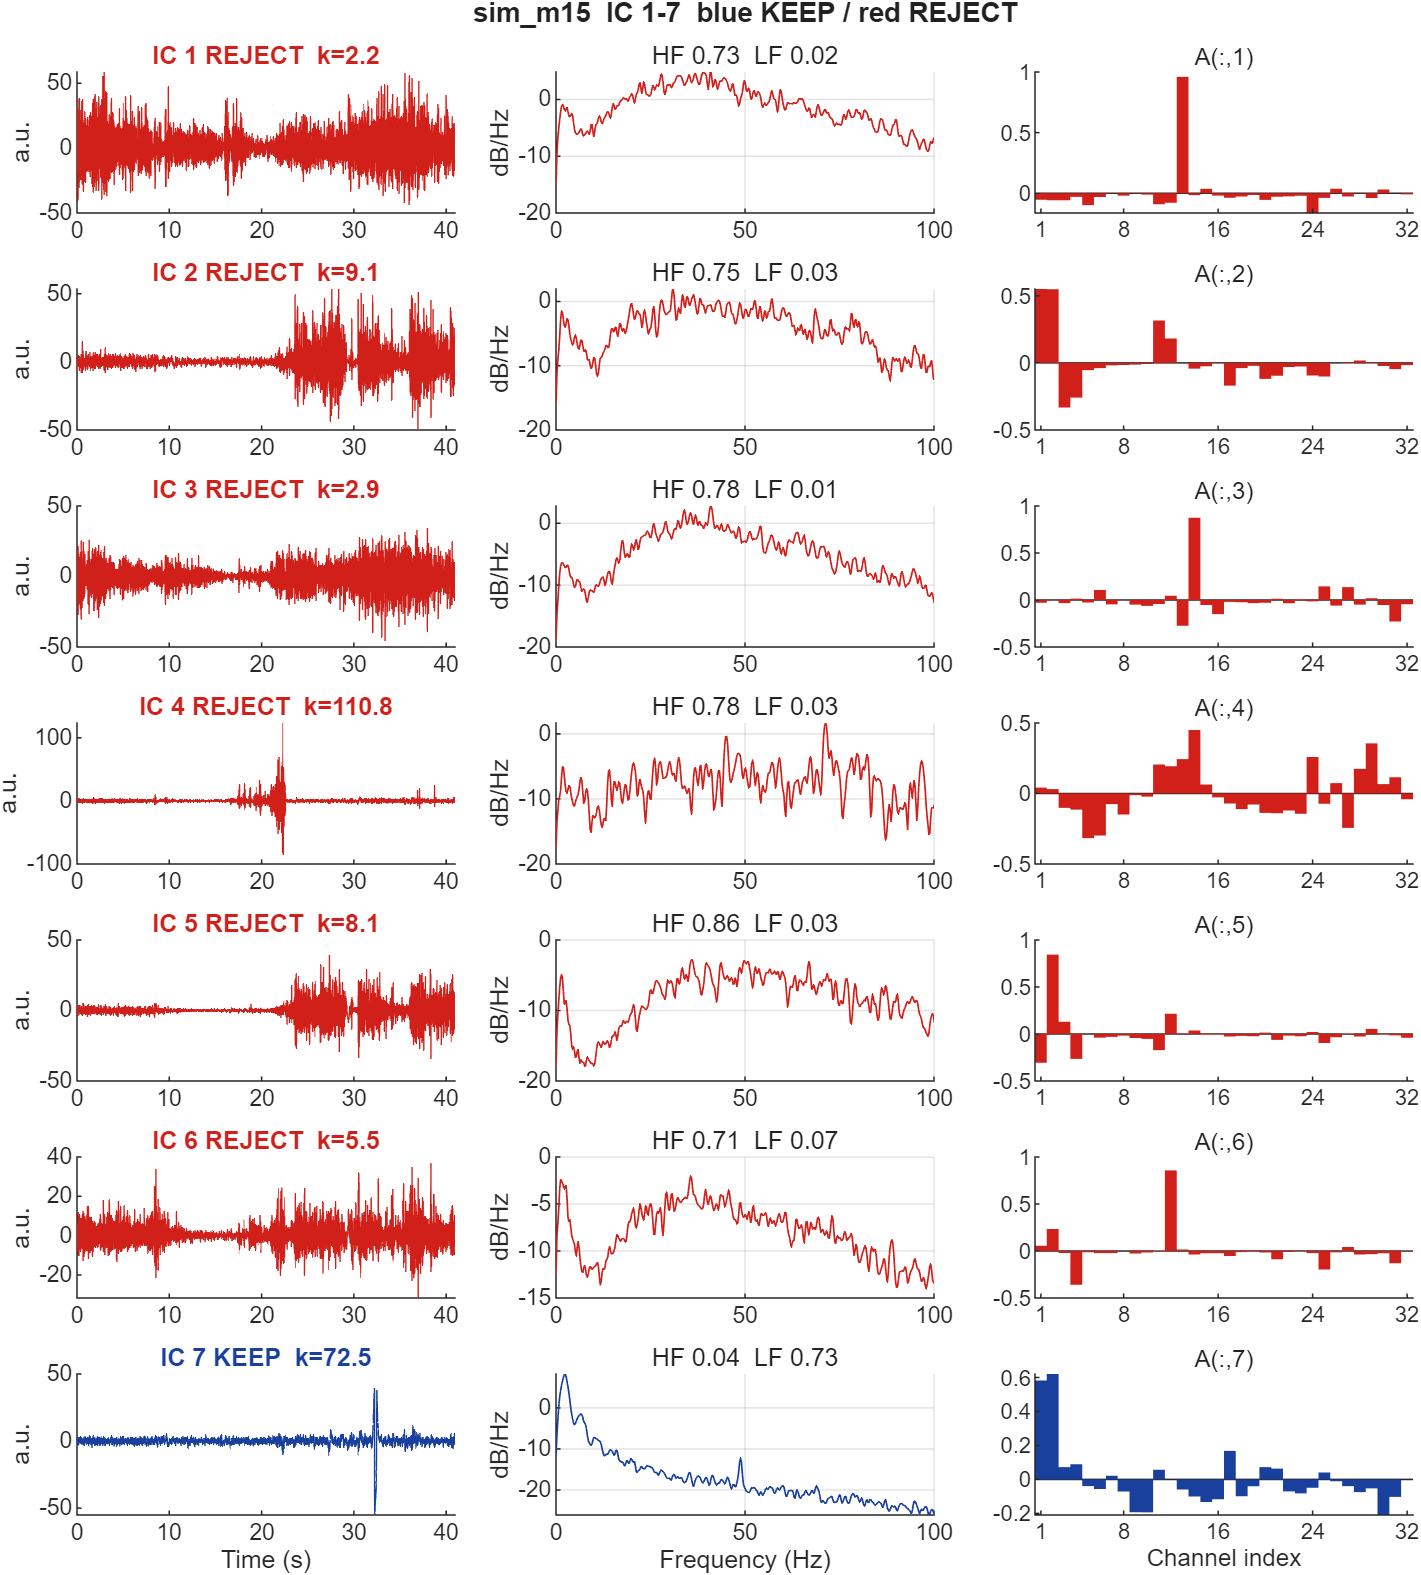
\includegraphics[height=0.80\textheight,width=0.95\textwidth,keepaspectratio]{fig21_sim_m15db_ic01_to_ic07.png}
\caption{Time course, PSD and mixing pattern of components components 1 to 7 in the $-15$~dB simulation.}
\label{fig:app21}
\end{figure}
\begin{figure}[p]
\centering
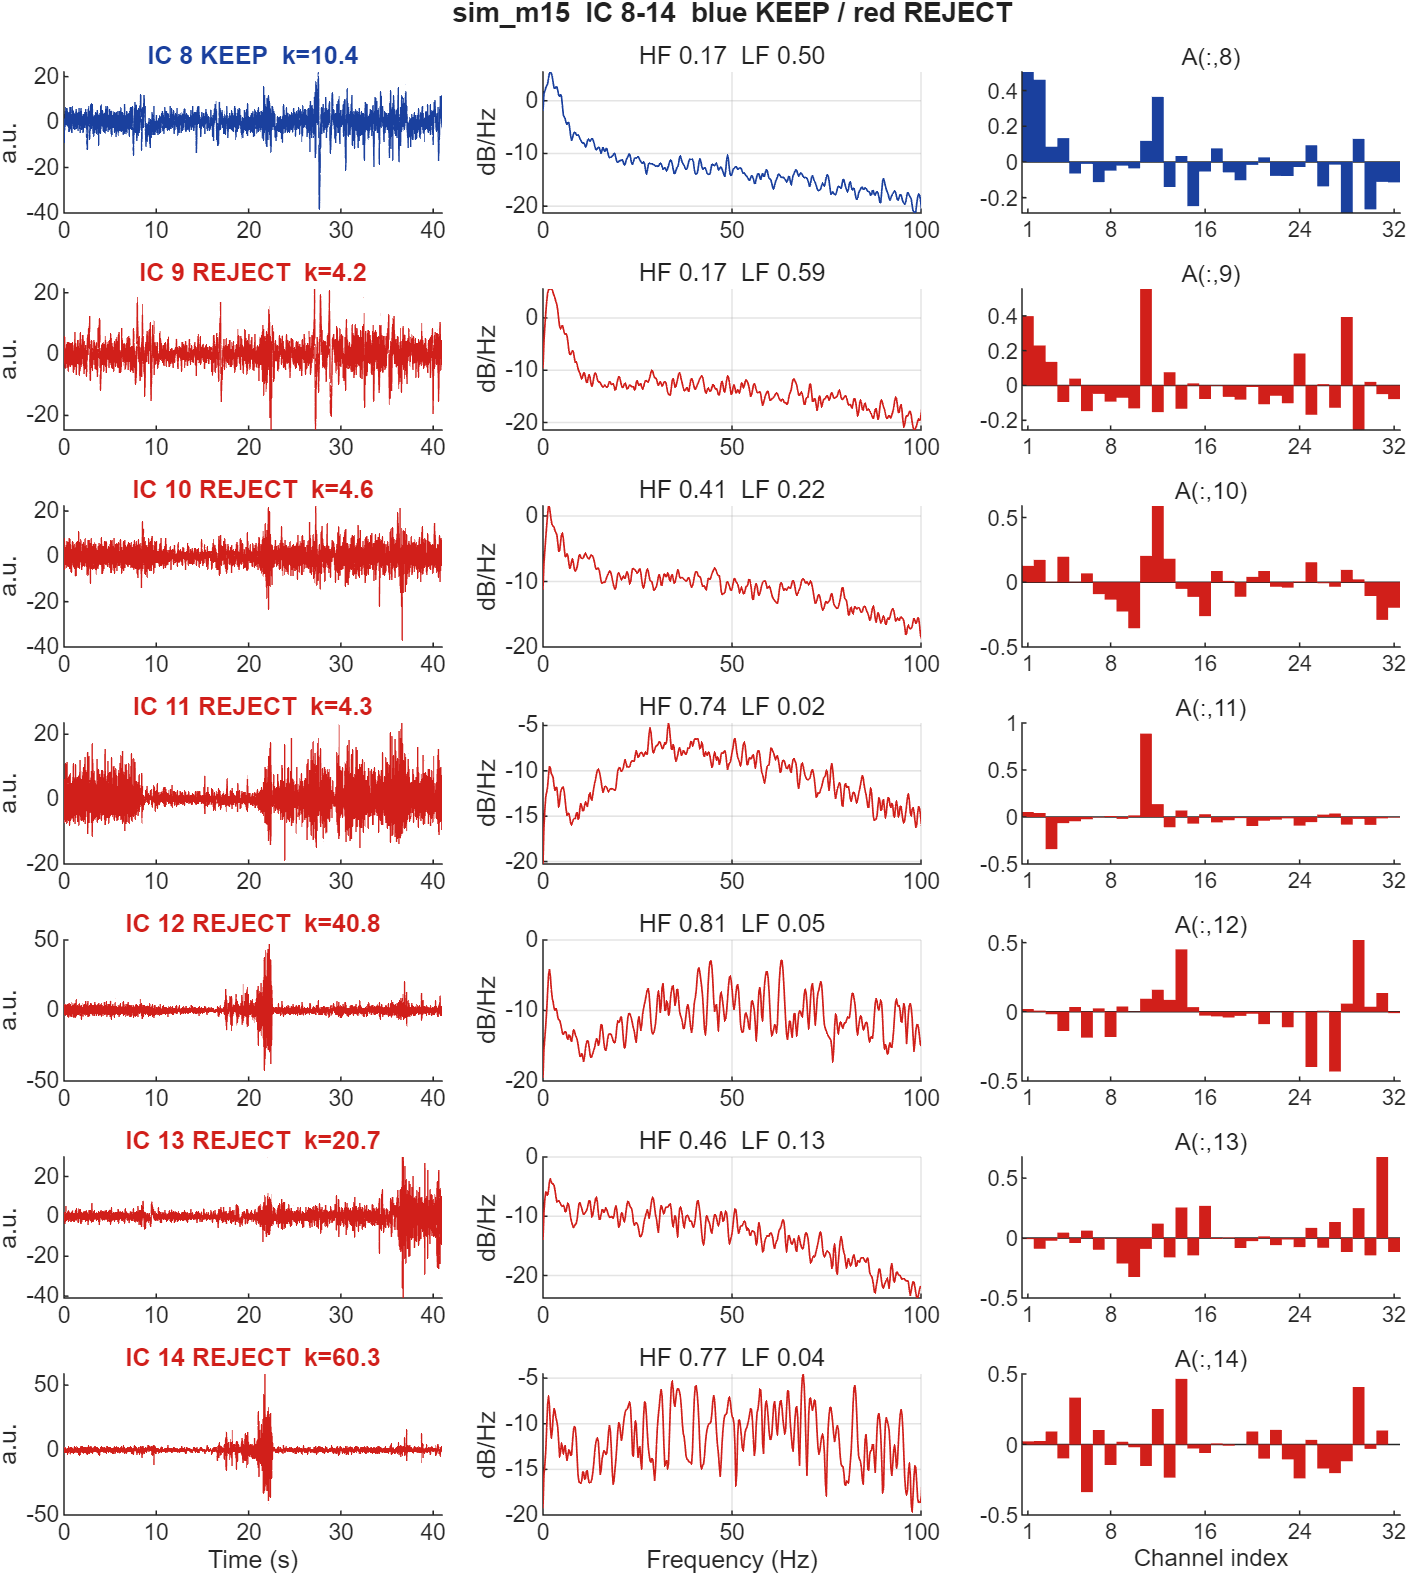
\includegraphics[height=0.80\textheight,width=0.95\textwidth,keepaspectratio]{fig22_sim_m15db_ic08_to_ic14.png}
\caption{Time course, PSD and mixing pattern of components components 8 to 14 in the $-15$~dB simulation.}
\label{fig:app22}
\end{figure}
\begin{figure}[p]
\centering
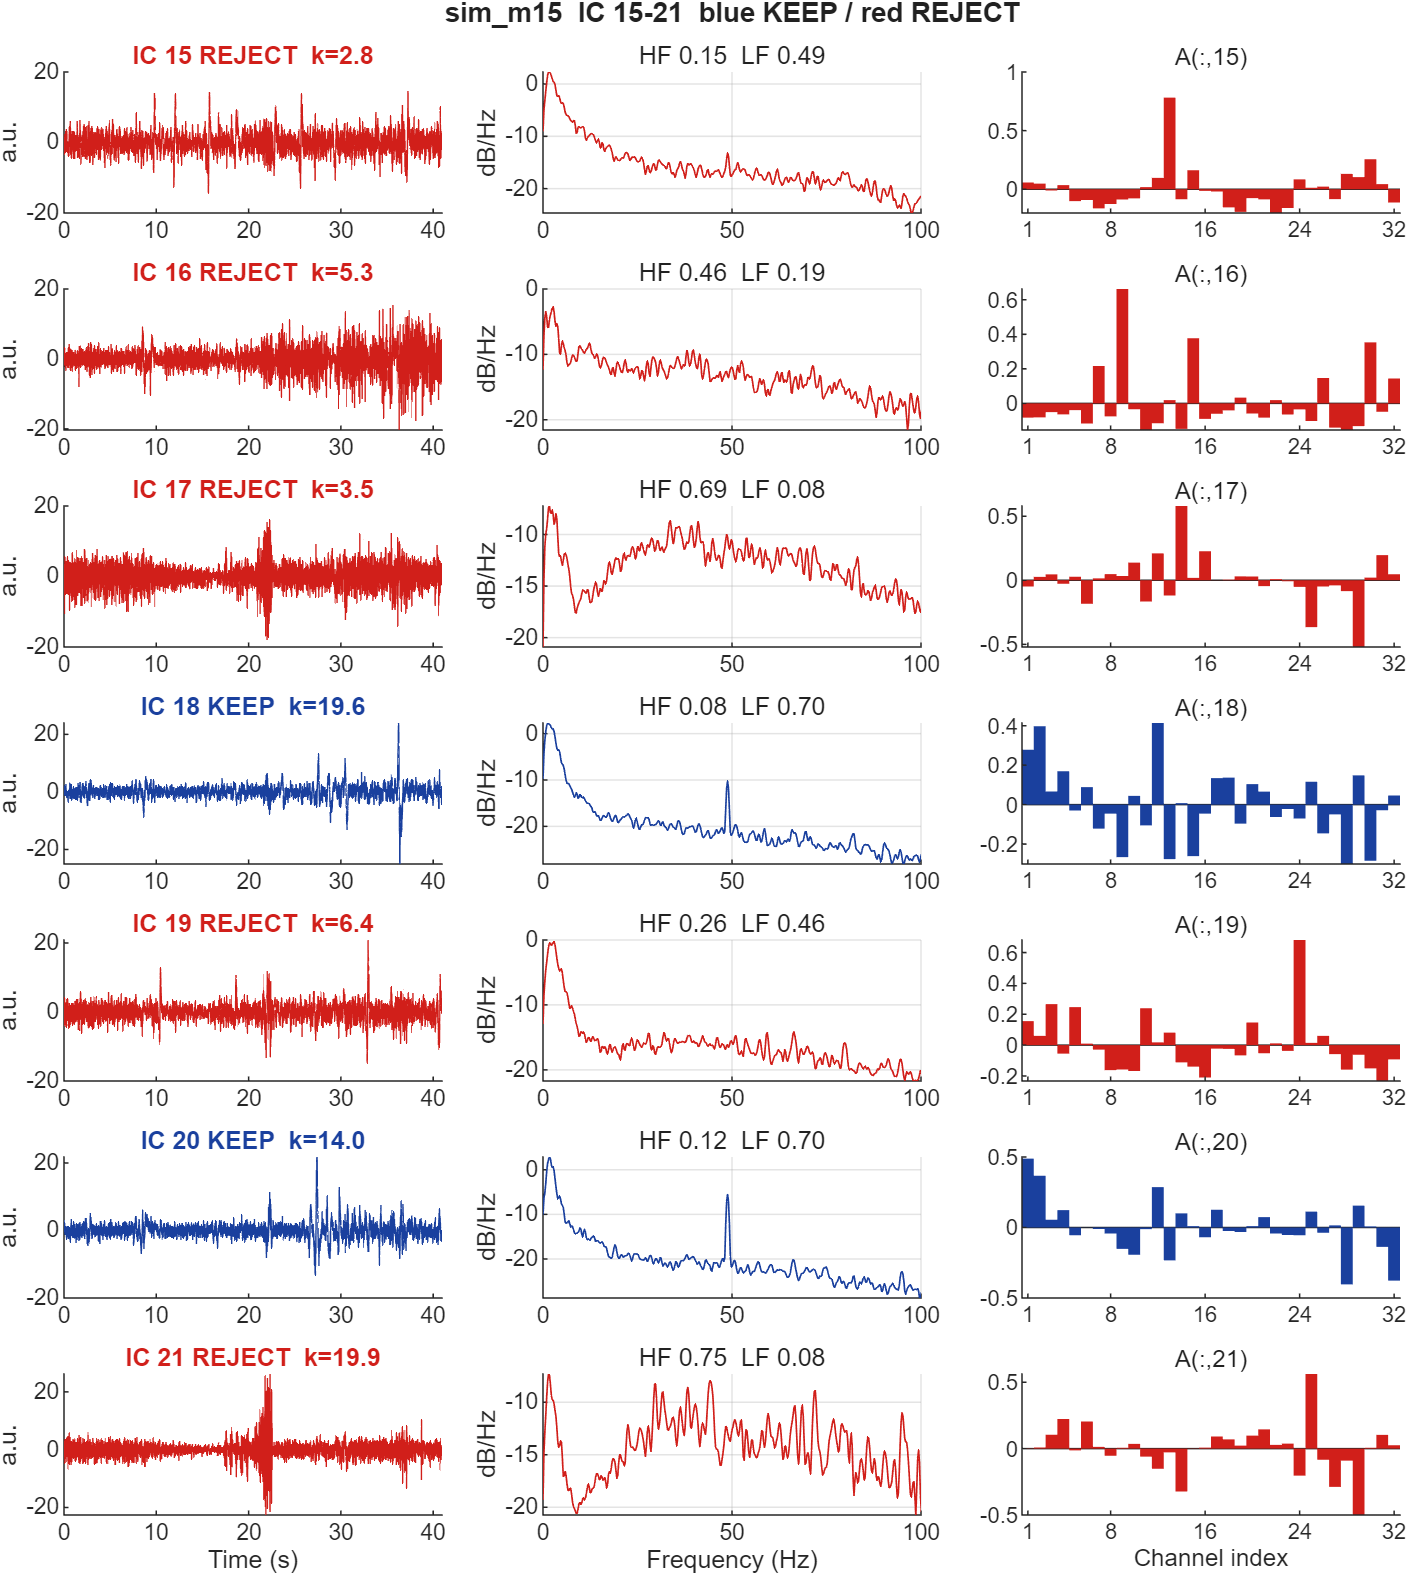
\includegraphics[height=0.80\textheight,width=0.95\textwidth,keepaspectratio]{fig23_sim_m15db_ic15_to_ic21.png}
\caption{Time course, PSD and mixing pattern of components components 15 to 21 in the $-15$~dB simulation.}
\label{fig:app23}
\end{figure}
\begin{figure}[p]
\centering
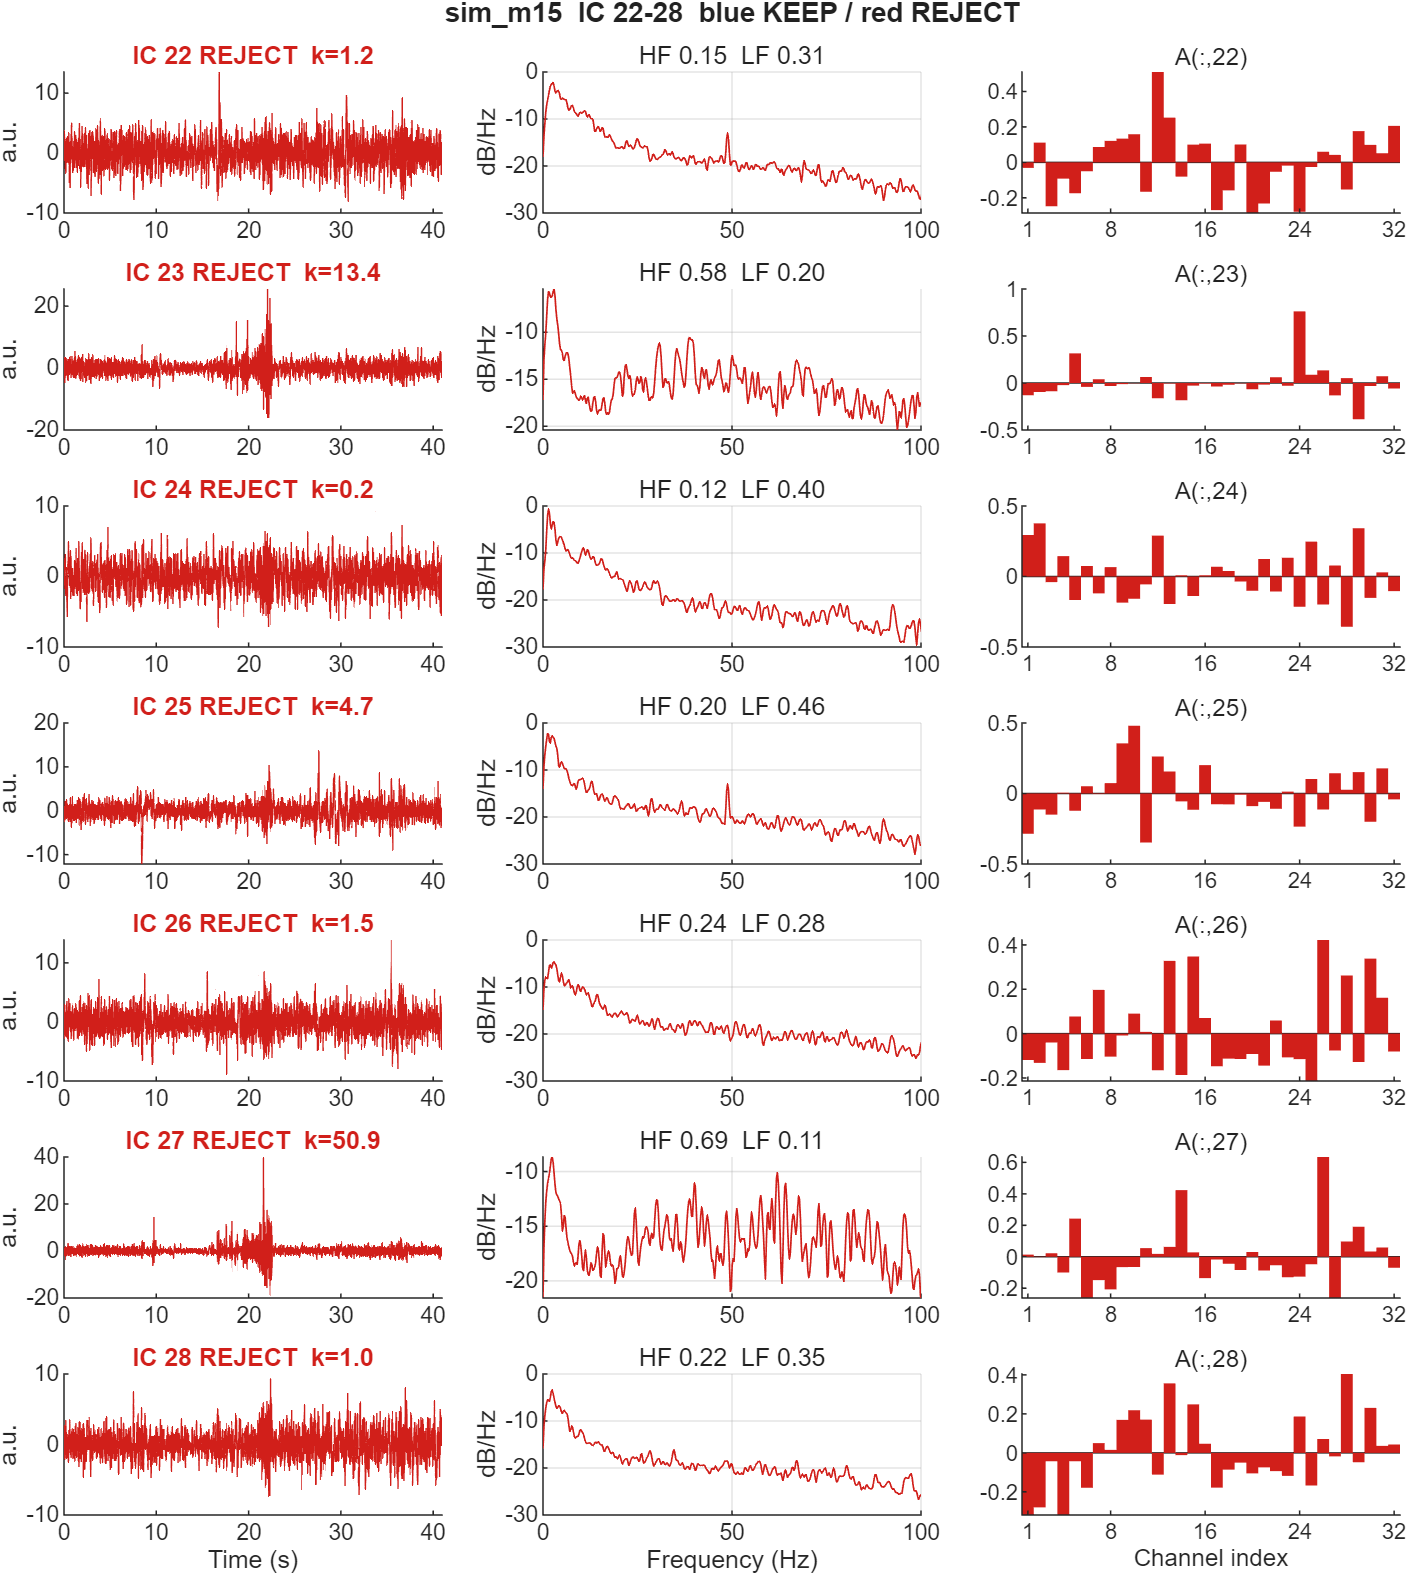
\includegraphics[height=0.80\textheight,width=0.95\textwidth,keepaspectratio]{fig24_sim_m15db_ic22_to_ic28.png}
\caption{Time course, PSD and mixing pattern of components components 22 to 28 in the $-15$~dB simulation.}
\label{fig:app24}
\end{figure}
\begin{figure}[p]
\centering
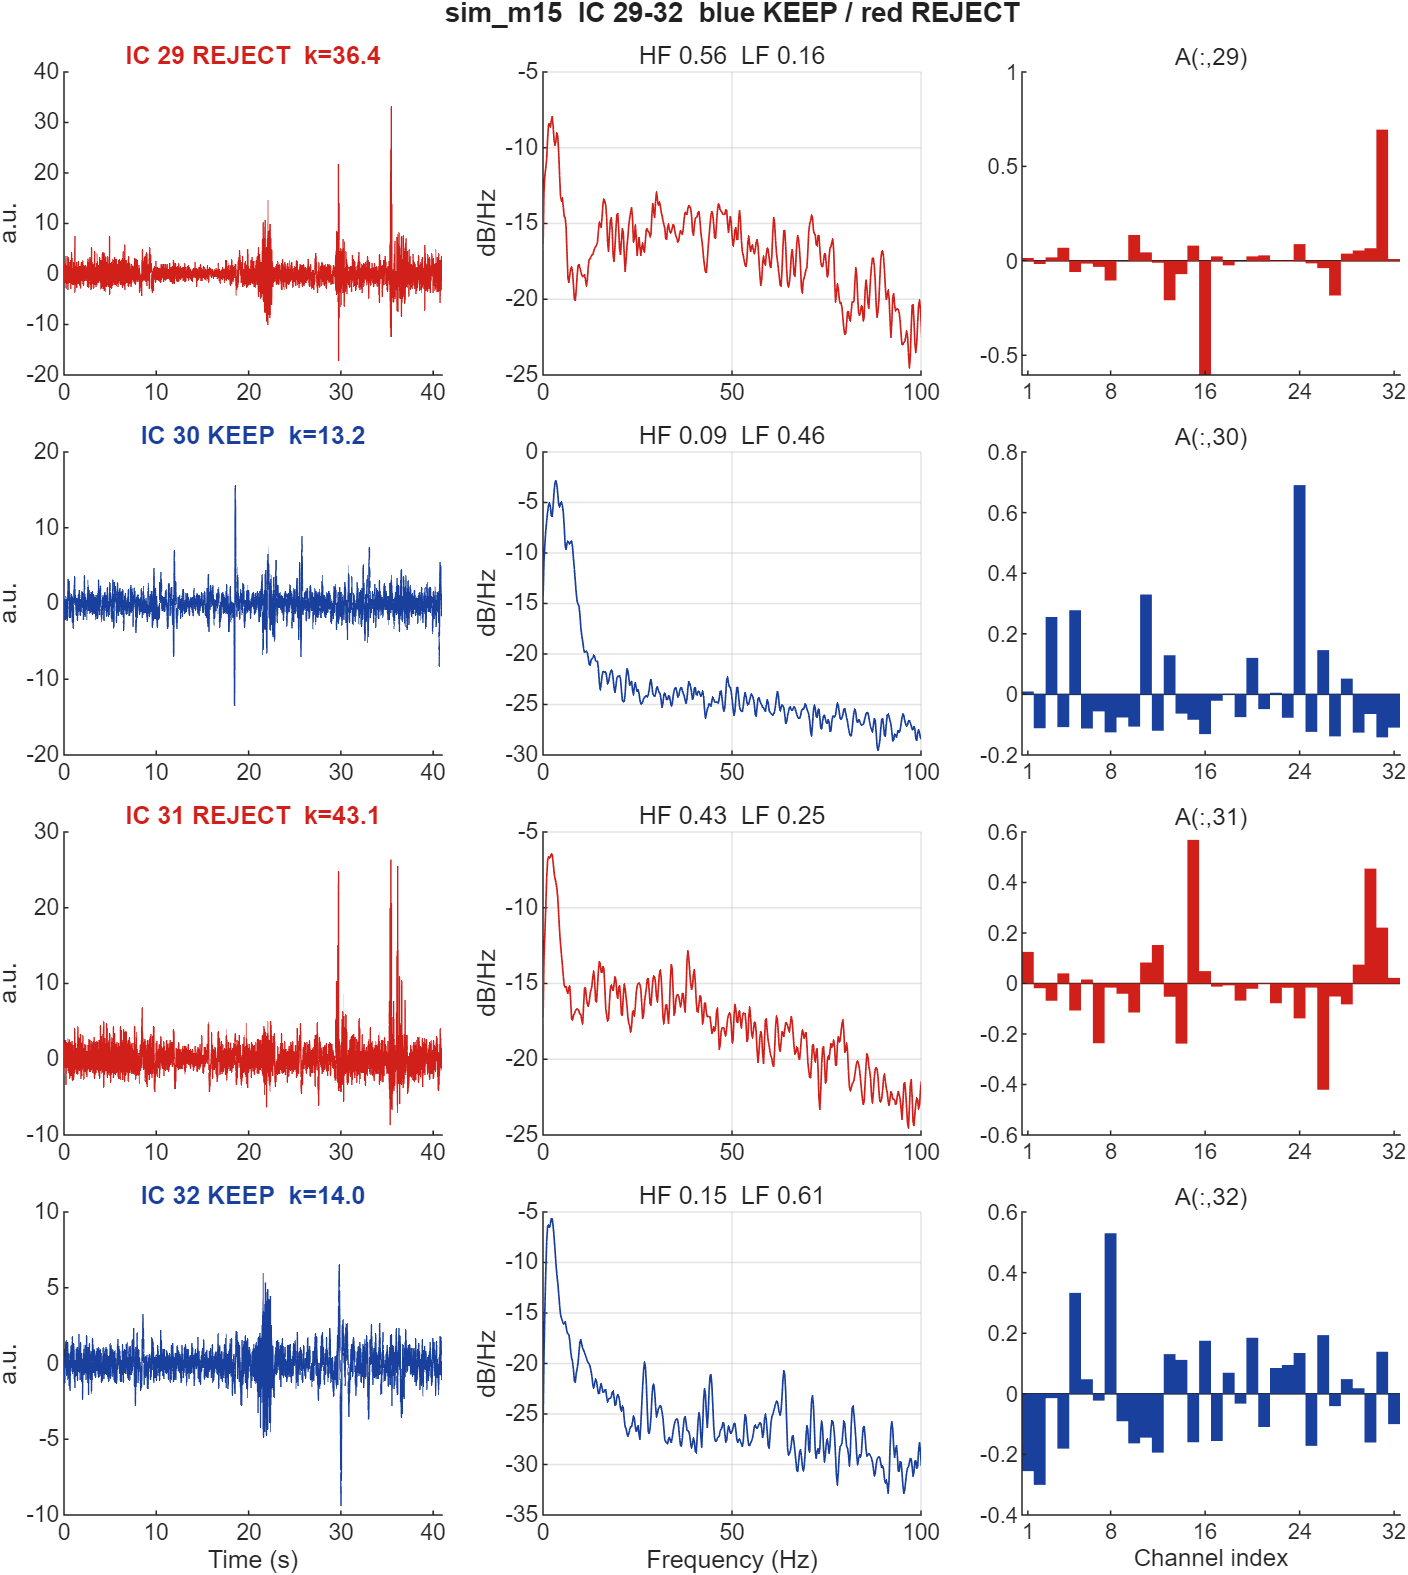
\includegraphics[height=0.80\textheight,width=0.95\textwidth,keepaspectratio]{fig25_sim_m15db_ic29_to_ic32.png}
\caption{Time course, PSD and mixing pattern of components components 29 to 32 in the $-15$~dB simulation.}
\label{fig:app25}
\end{figure}
\begin{figure}[p]
\centering
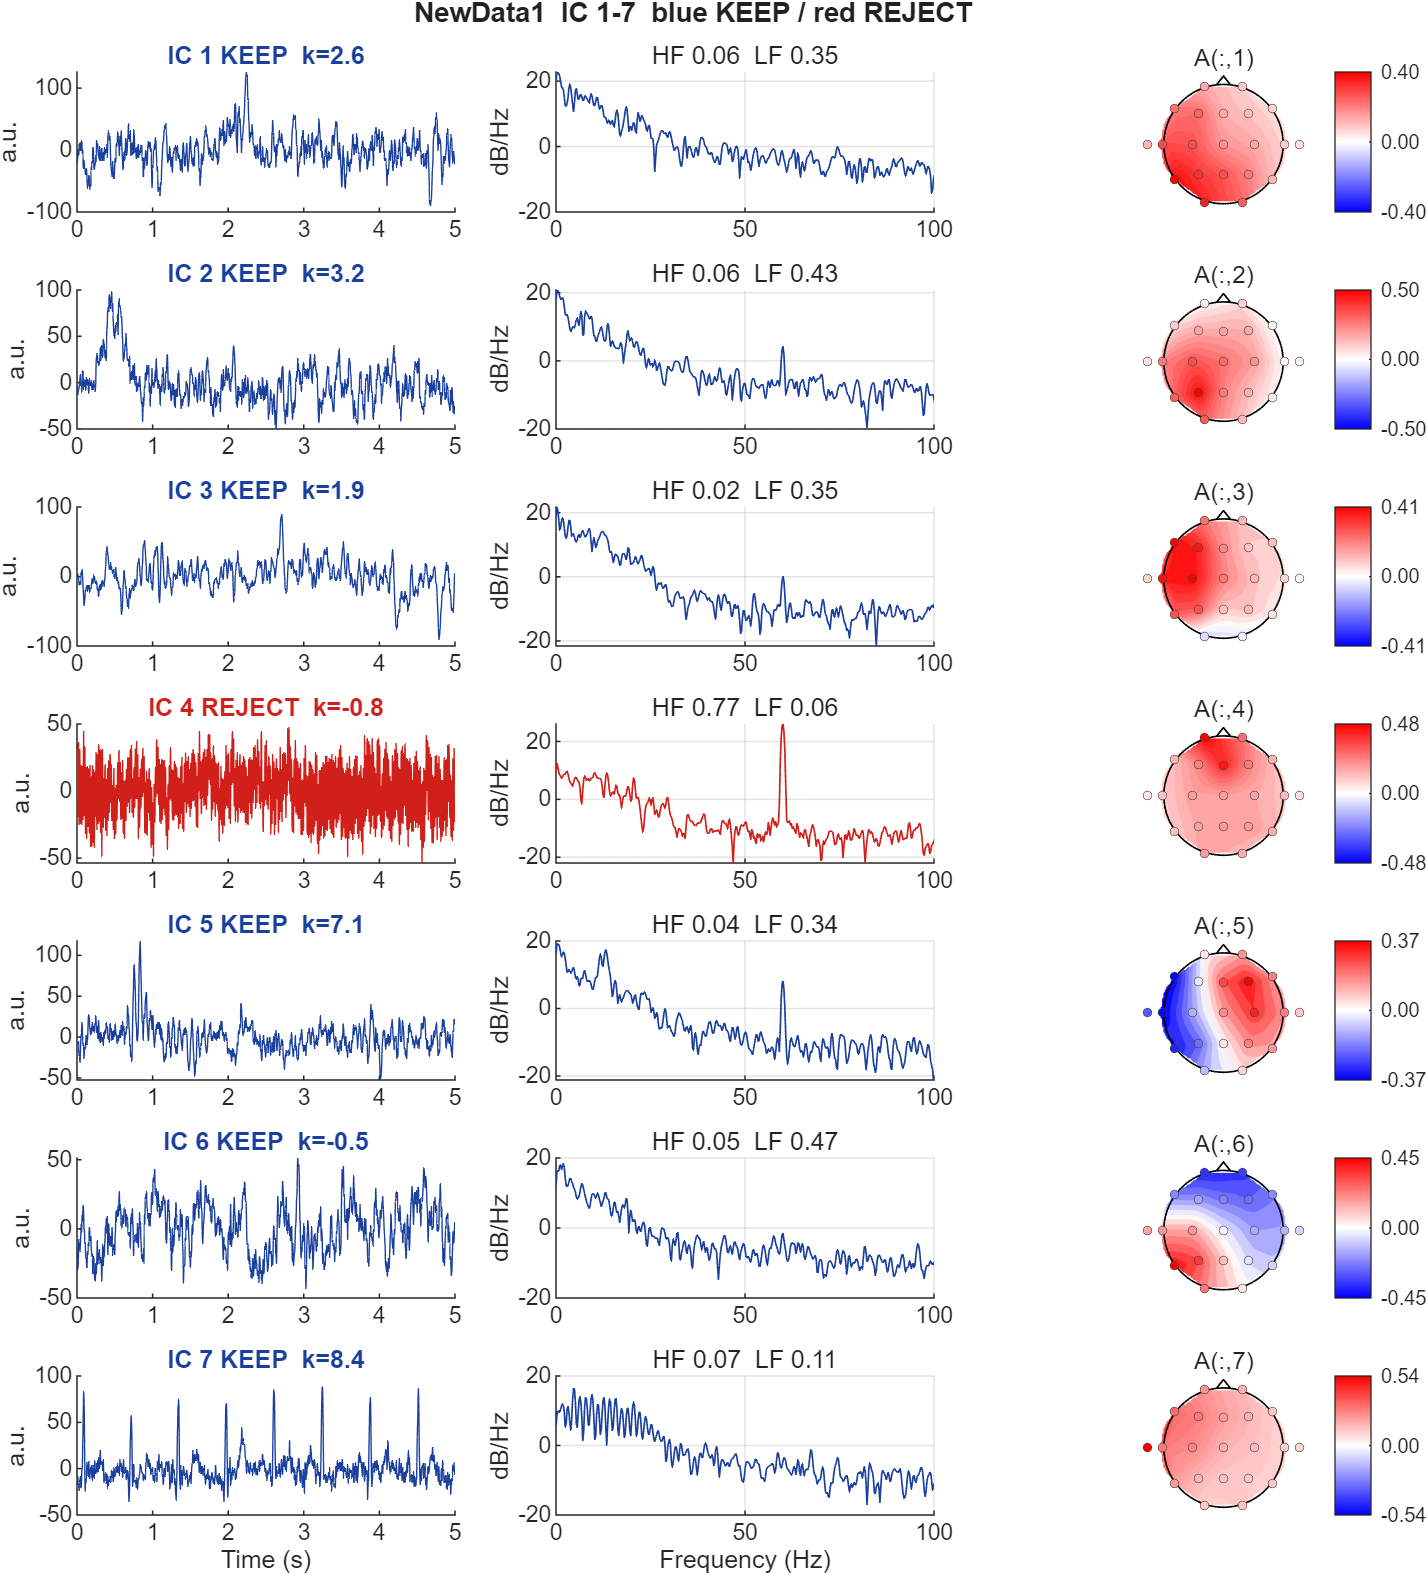
\includegraphics[height=0.80\textheight,width=0.95\textwidth,keepaspectratio]{fig26_newdata1_ic01_to_ic07.png}
\caption{Time course, PSD and mixing pattern of components components 1 to 7 in the real recording NewData1.}
\label{fig:app26}
\end{figure}
\begin{figure}[p]
\centering
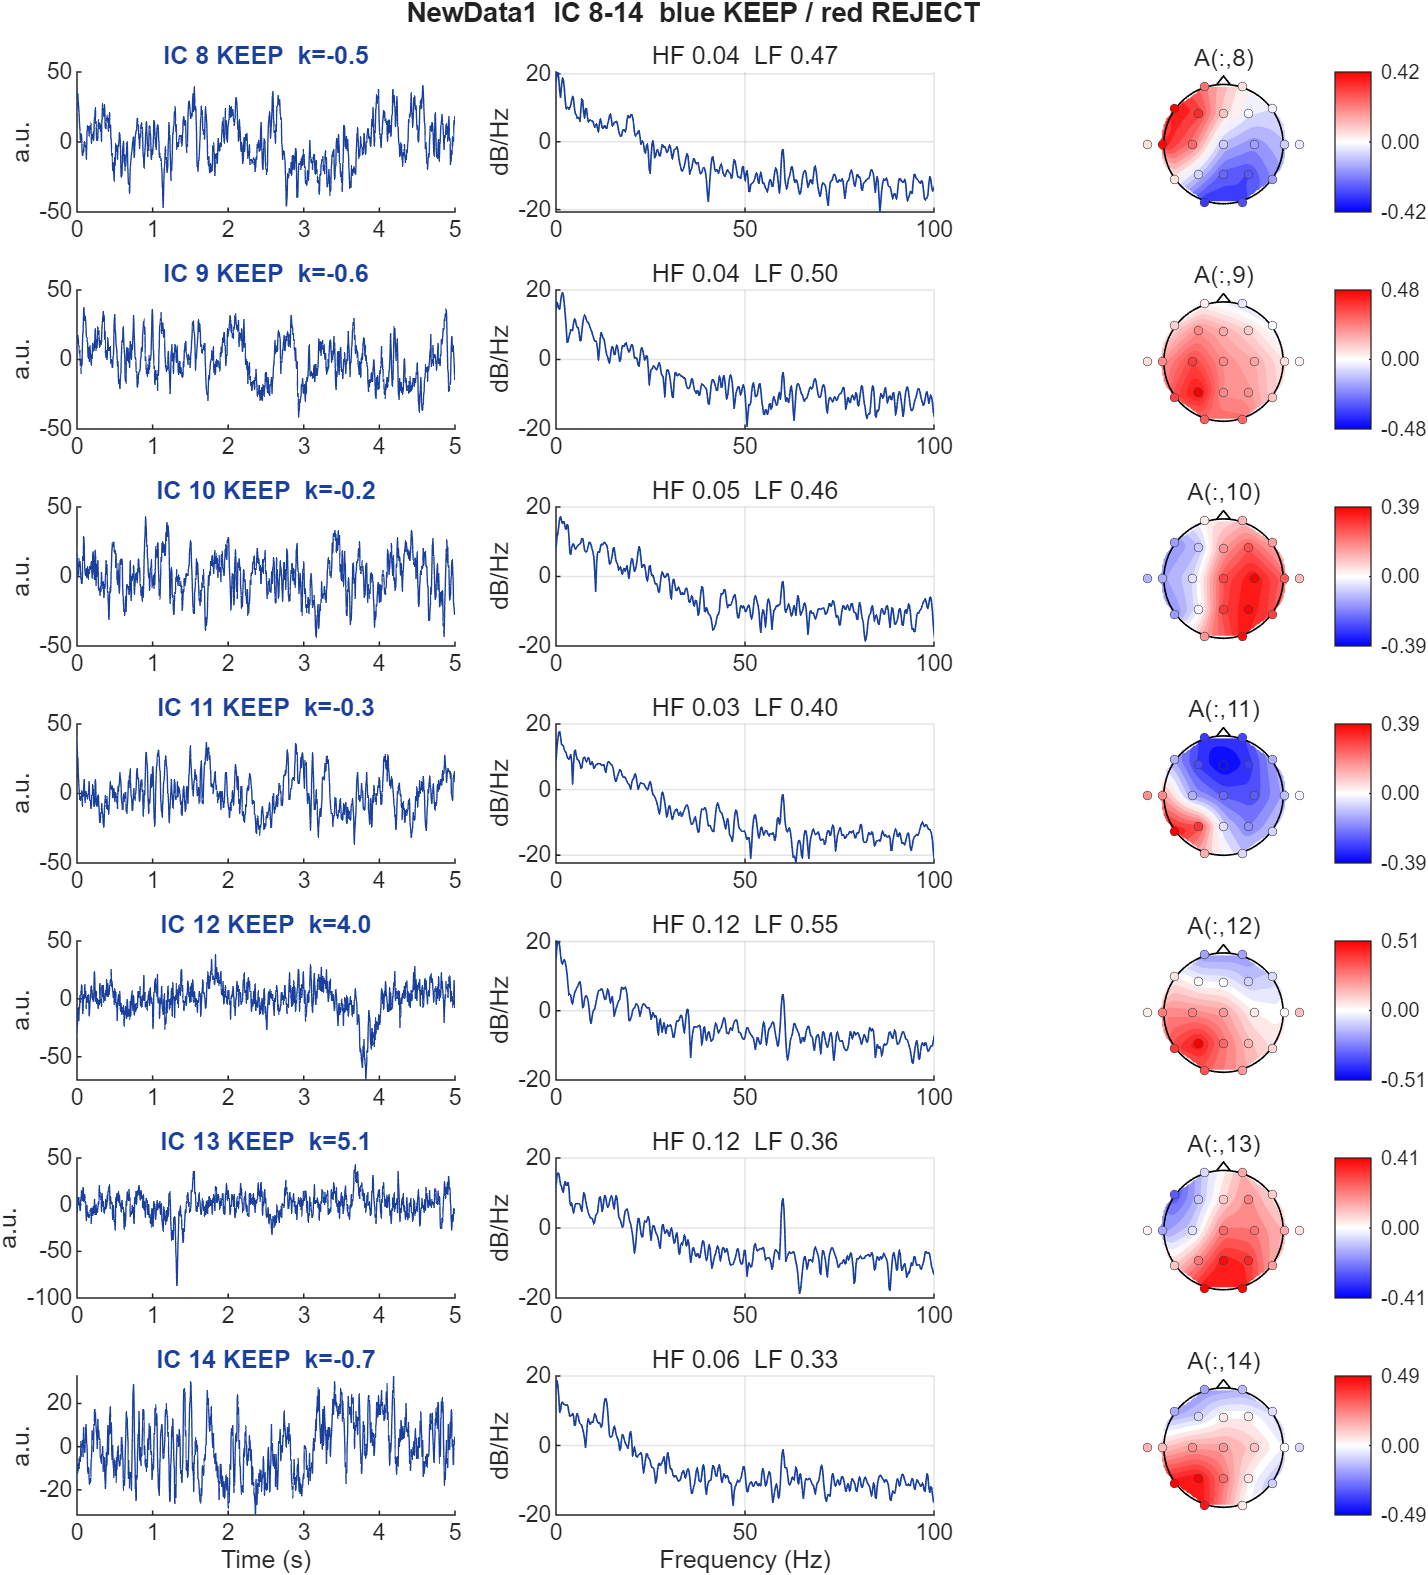
\includegraphics[height=0.80\textheight,width=0.95\textwidth,keepaspectratio]{fig27_newdata1_ic08_to_ic14.png}
\caption{Time course, PSD and mixing pattern of components components 8 to 14 in the real recording NewData1.}
\label{fig:app27}
\end{figure}
\begin{figure}[p]
\centering
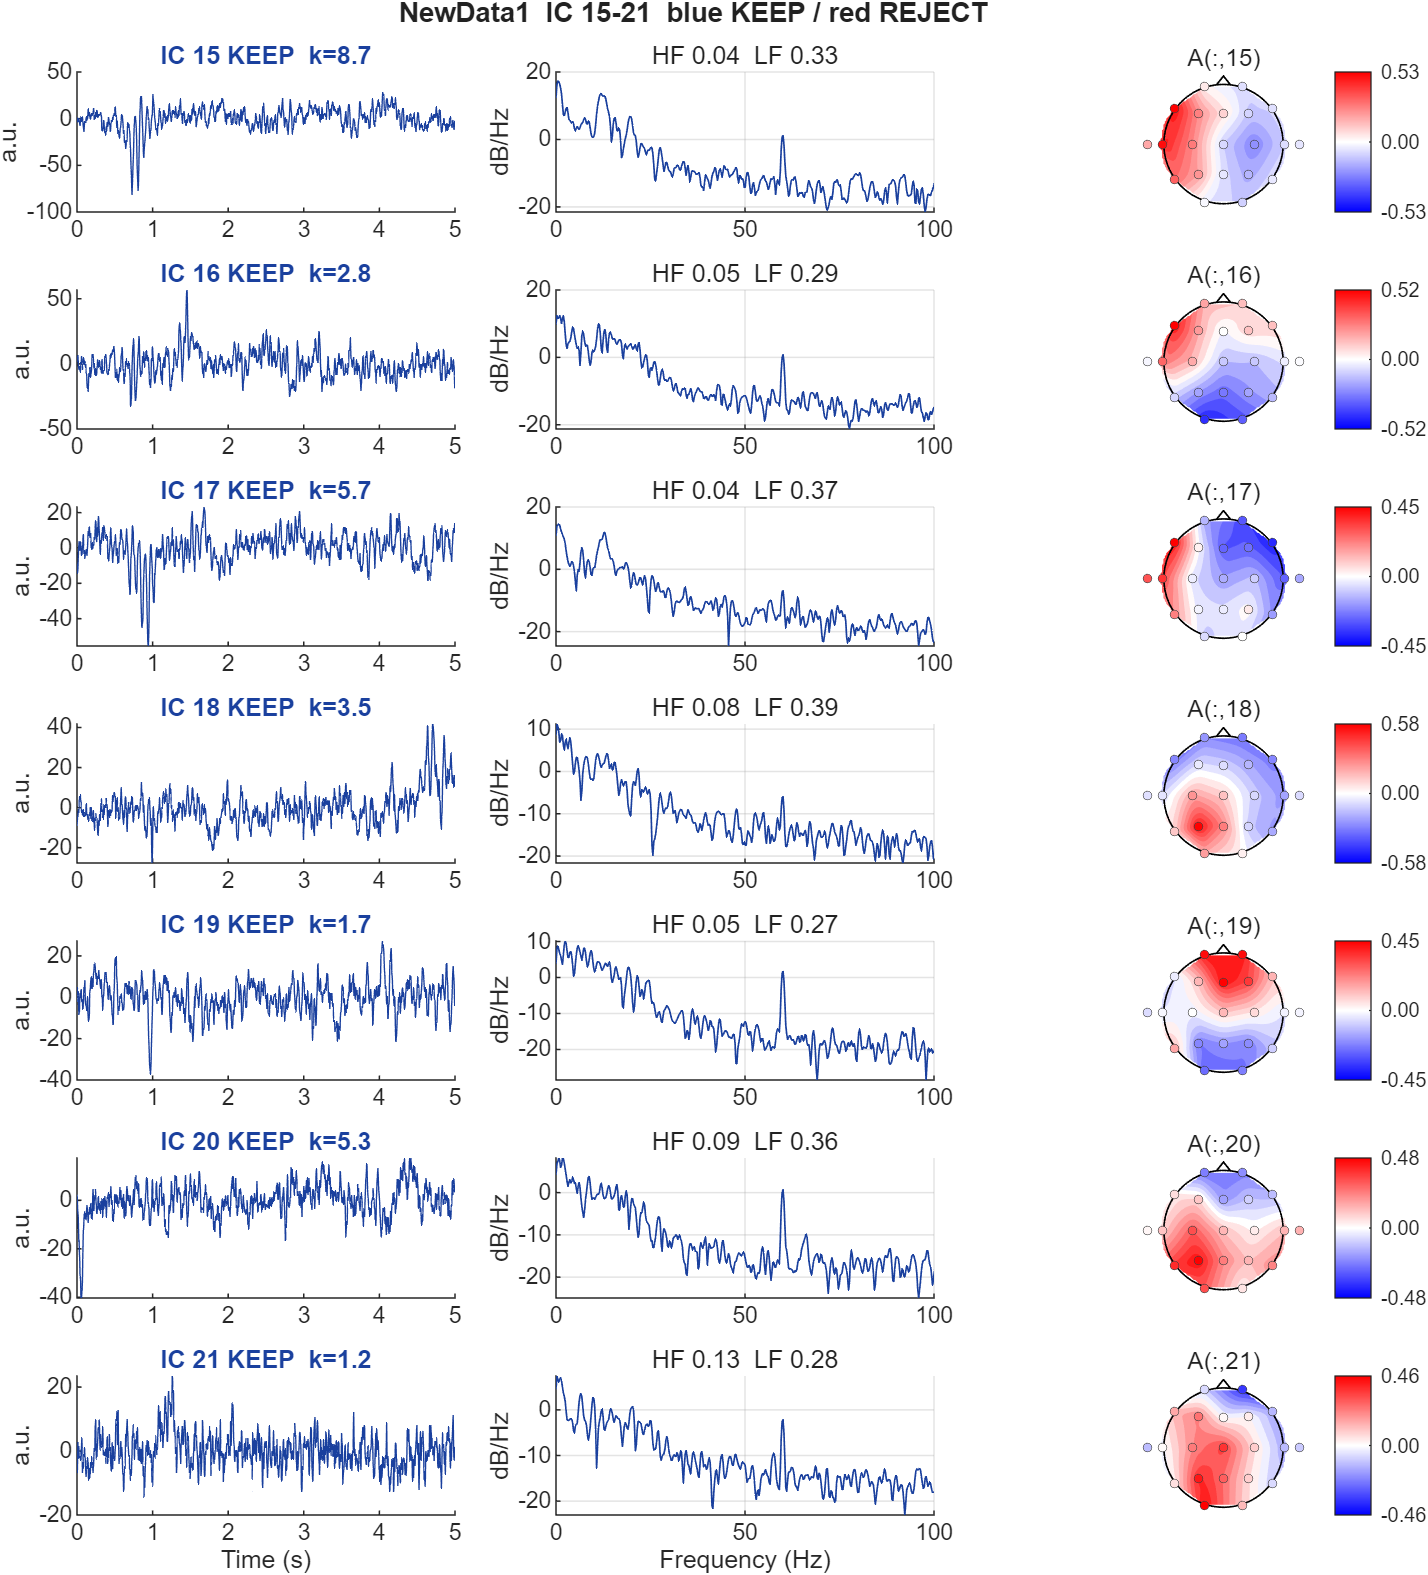
\includegraphics[height=0.80\textheight,width=0.95\textwidth,keepaspectratio]{fig28_newdata1_ic15_to_ic21.png}
\caption{Time course, PSD and mixing pattern of components components 15 to 21 in the real recording NewData1.}
\label{fig:app28}
\end{figure}
\begin{figure}[p]
\centering
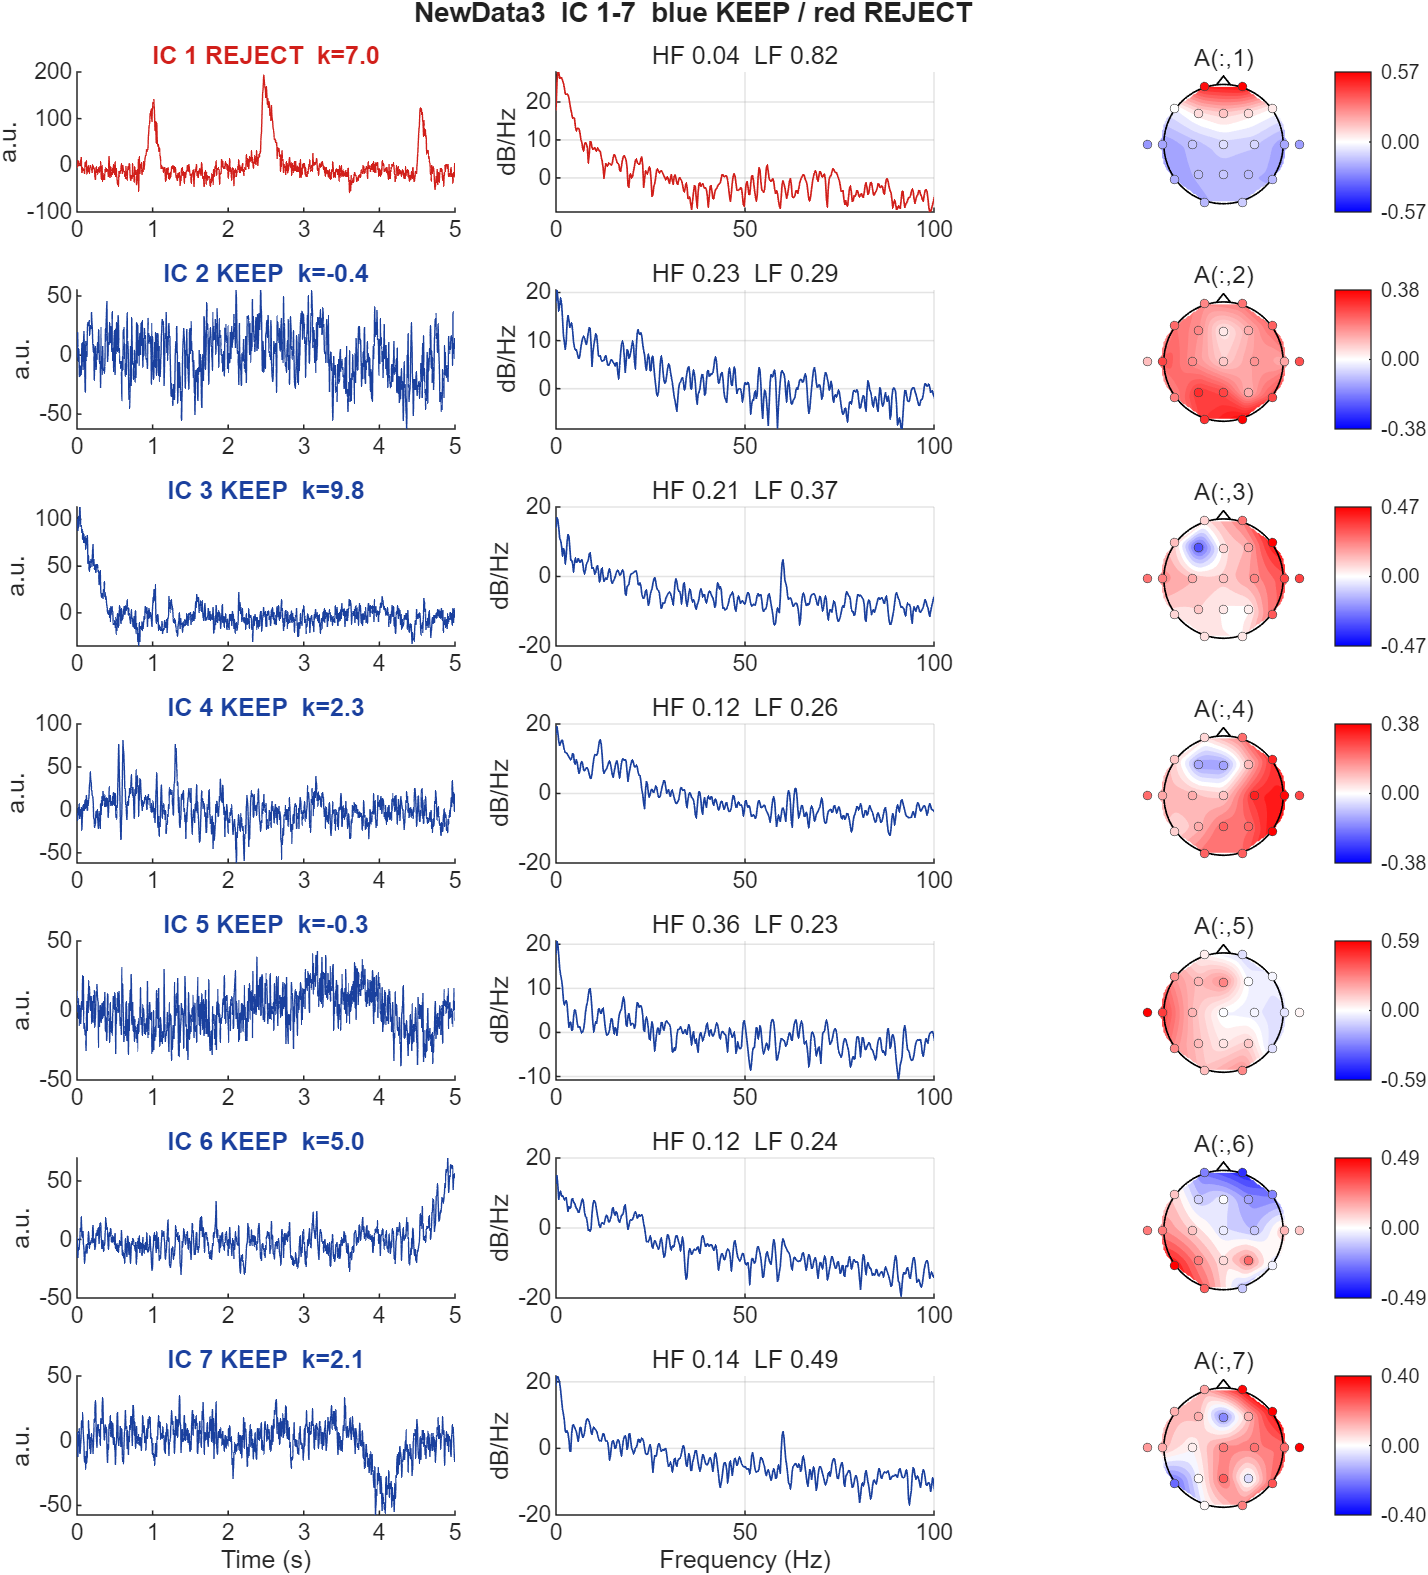
\includegraphics[height=0.80\textheight,width=0.95\textwidth,keepaspectratio]{fig29_newdata3_ic01_to_ic07.png}
\caption{Time course, PSD and mixing pattern of components components 1 to 7 in the real recording NewData3.}
\label{fig:app29}
\end{figure}
\begin{figure}[p]
\centering
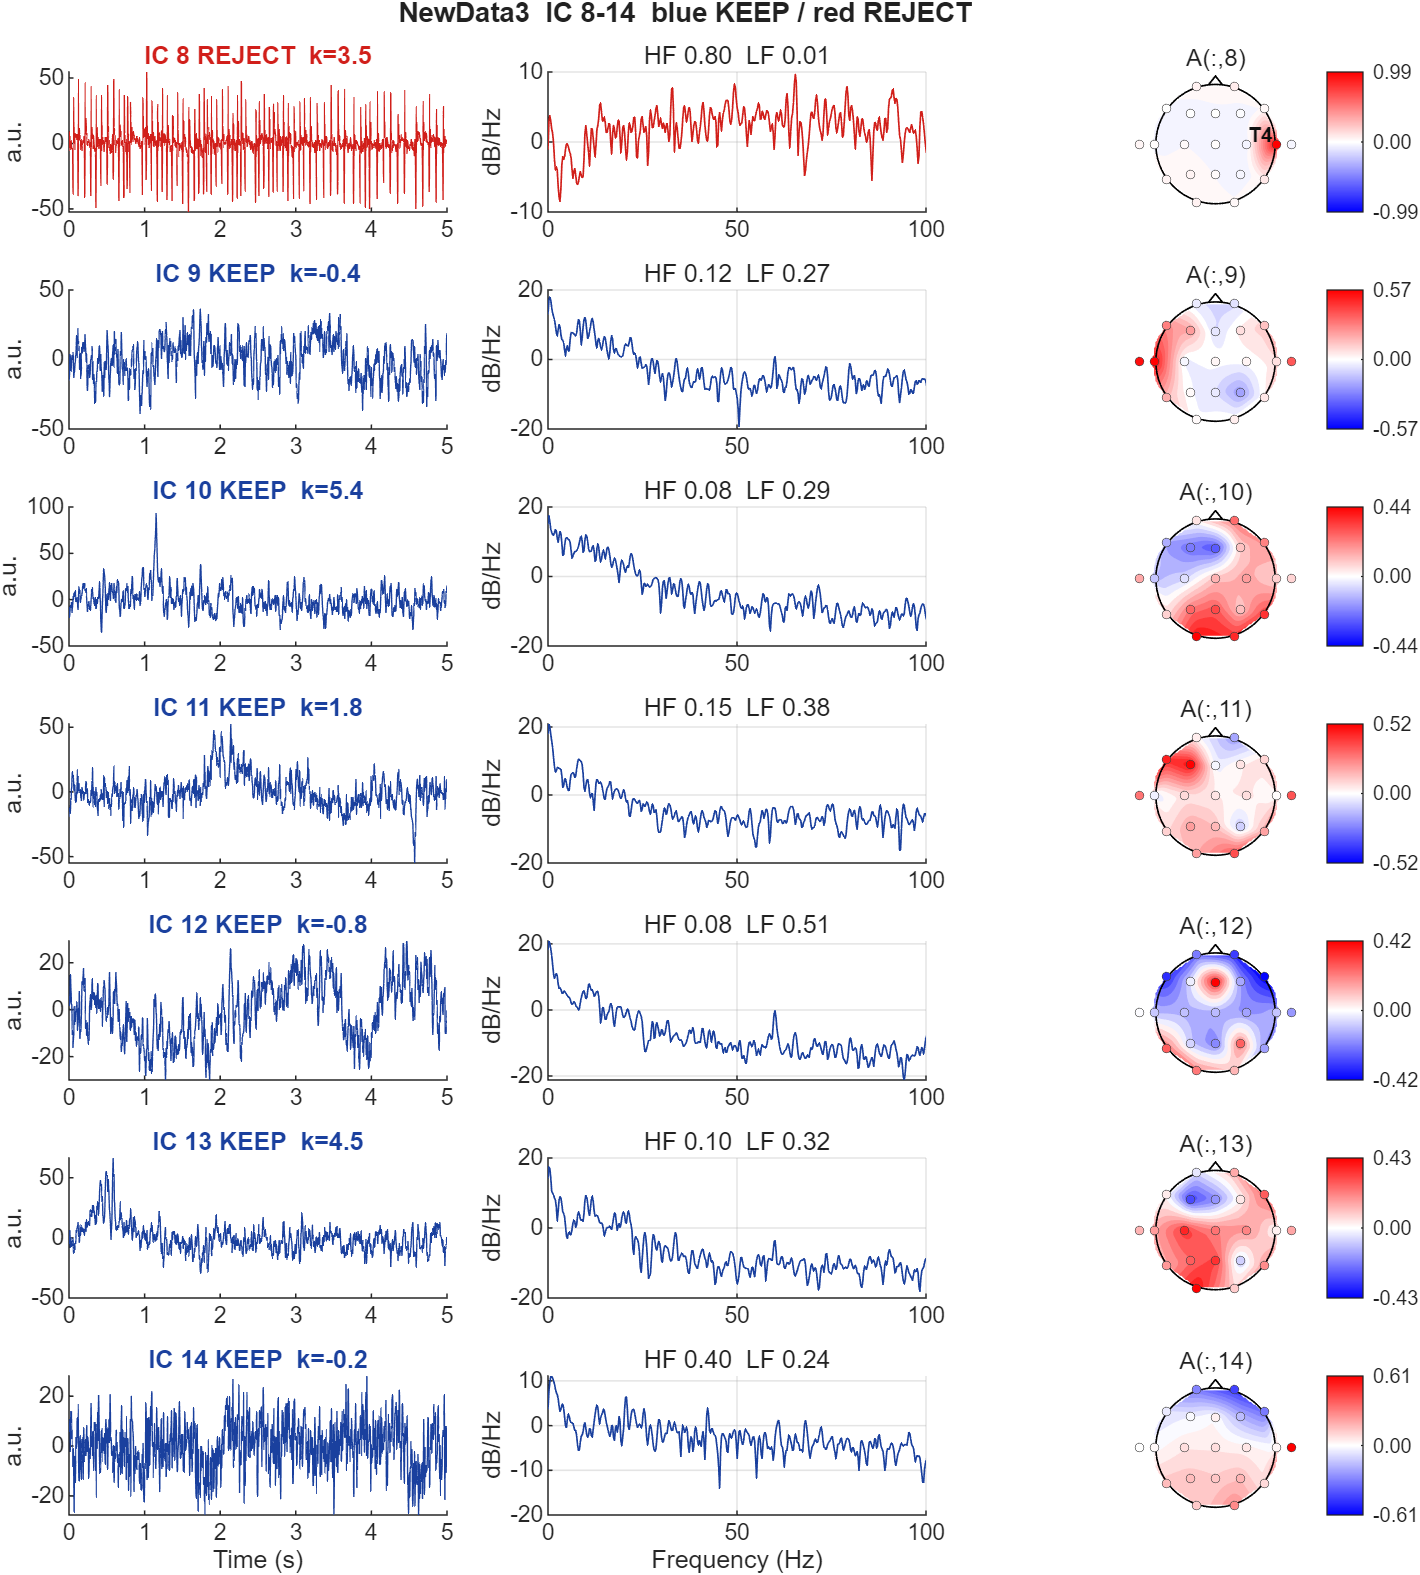
\includegraphics[height=0.80\textheight,width=0.95\textwidth,keepaspectratio]{fig30_newdata3_ic08_to_ic14.png}
\caption{Time course, PSD and mixing pattern of components components 8 to 14 in the real recording NewData3.}
\label{fig:app30}
\end{figure}
\begin{figure}[p]
\centering
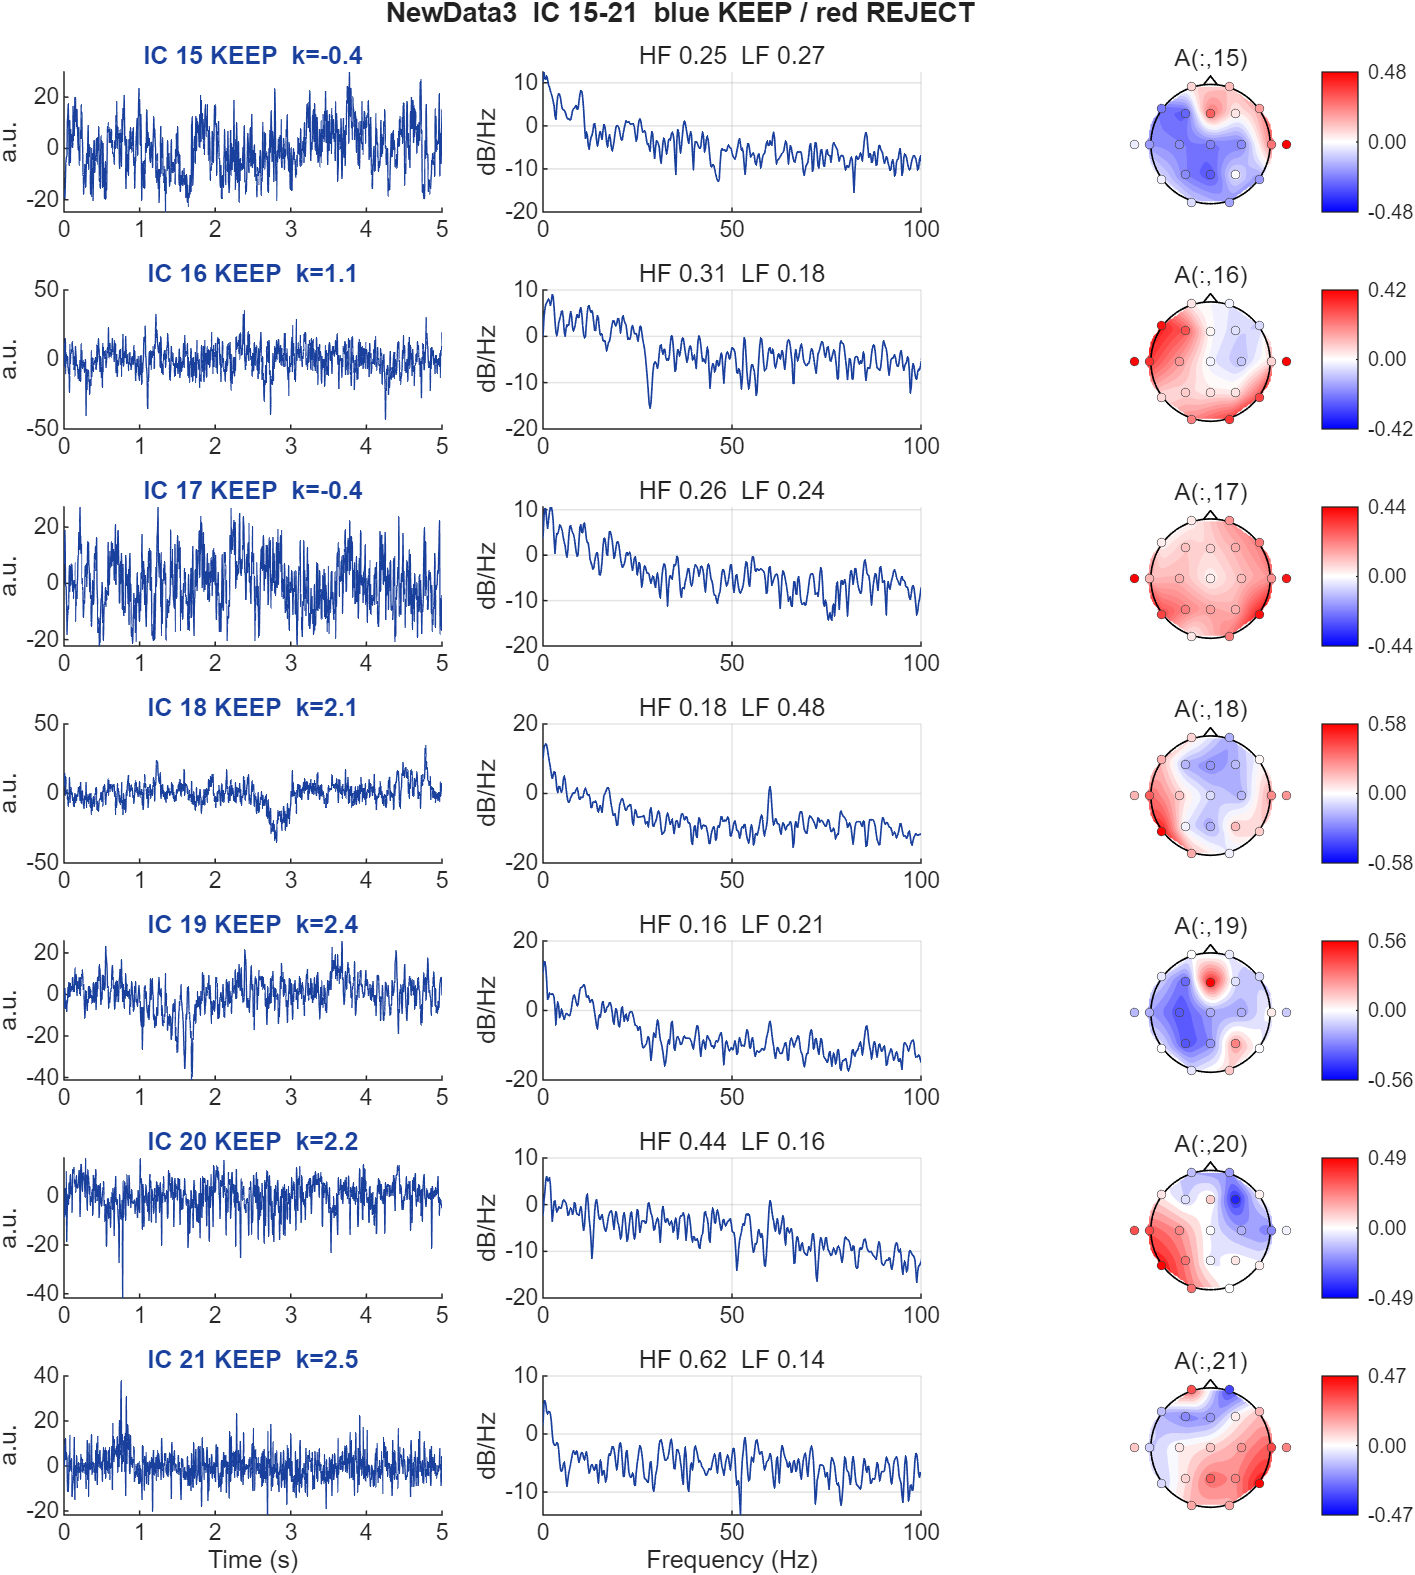
\includegraphics[height=0.80\textheight,width=0.95\textwidth,keepaspectratio]{fig31_newdata3_ic15_to_ic21.png}
\caption{Time course, PSD and mixing pattern of components components 15 to 21 in the real recording NewData3.}
\label{fig:app31}
\end{figure}

\clearpage
\section*{References}
\addcontentsline{toc}{section}{References}

\begin{enumerate}[label={[\arabic*]},leftmargin=2.4em,itemsep=0.5em]
\item Lab manual of Experiment 2: \emph{Noises and Artifacts of the EEG Signal and Methods for Removing Them}, Medical Signal and Image Processing Lab, Sharif University of Technology, file \texttt{Lab2.pdf}, Parts 1 and 2.
\item Hajipour, S. \emph{EEG Pre Processing and Artifact Removal}. Sharif University of Technology, 2024. Course slides, especially slides 16--23. Supplied file \texttt{EEG\_Pre-Processing.pdf}.
\item Comon, P. Independent component analysis, a new concept? \emph{Signal Processing} 36(3), 287--314, 1994. DOI \href{https://doi.org/10.1016/0165-1684(94)90029-9}{10.1016/0165-1684(94)90029-9}.
\item MathWorks. \emph{pwelch: Welch power spectral density estimate}. MATLAB Signal Processing Toolbox documentation. \url{https://www.mathworks.com/help/signal/ref/pwelch.html}
\item Pion-Tonachini, L., Kreutz-Delgado, K., and Makeig, S. ICLabel: An automated electroencephalographic independent component classifier, dataset, and website. \emph{NeuroImage} 198, 181--197, 2019. DOI \href{https://doi.org/10.1016/j.neuroimage.2019.05.026}{10.1016/j.neuroimage.2019.05.026}.
\end{enumerate}

The source of the data and of the algorithm accompanying the experiment is the folders \texttt{Lab2\_1} and \texttt{Lab2\_2}. The numbers and the decisions were extracted from \texttt{summary.json}, the \texttt{metrics} and \texttt{decisions} tables and the MAT files of the final run. The tools that were run are specified in the text and in Appendix~A.

\end{document}
